% !TeX program = lualatex
\documentclass[10pt,a4paper]{report}

\usepackage{fontspec}
\setmainfont{Arial}

% Ensure the first paragraph in each section or chapter is indented
\usepackage{indentfirst}

% Set Polish as the main language and English as a secondary language
\usepackage{polyglossia}
\setdefaultlanguage{polish}

% Page geometry settings
\usepackage{geometry}
\geometry{
    a4paper,
    top=2.5cm,
    bottom=2.5cm,
    inner=3.5cm,
    outer=2.5cm
}

% Line spacing
\usepackage{setspace}
\setstretch{1.5}

% Custom headers and footers
\usepackage{fancyhdr}
\pagestyle{fancy}
\fancyhf{}
\fancyfoot[C]{\thepage}
\fancypagestyle{plain}{
    \fancyhf{}
    \fancyfoot[C]{\thepage}
}
\renewcommand{\headrulewidth}{0pt}

% Paragraph formatting: indentation and spacing
\usepackage{parskip}
\setlength{\parindent}{1.25cm}
\setlength{\parskip}{0pt}
\raggedbottom

% Define custom colors according to the University's guidelines
\usepackage{xcolor}
\definecolor{pantone540}{HTML}{002B5C}
\definecolor{pantoneGray}{HTML}{75787B}
\definecolor{pantone1797}{HTML}{C8102E}

% Enable graphics support and define image path
\usepackage{graphicx}
\graphicspath{{assets/images/}}

% Configure captions for tables and figures
\usepackage{caption}
\captionsetup[table]{position=above}
\captionsetup[figure]{position=below}

% Enable PDF inclusion for the title page
\usepackage{pdfpages}

% Customize section and chapter titles
\usepackage{titlesec}

\titleformat{\chapter}[hang]{\bfseries\Large\MakeUppercase}{\thechapter.}{1em}{}{}
\titlespacing*{\chapter}{0pt}{*3}{*2}

\titleformat{\section}[hang]{\bfseries\itshape\large}{\thesection}{1em}{}{}
\titlespacing*{\section}{0pt}{*2}{*1.5}

\titleformat{\subsection}[hang]{\itshape\normalsize}{\thesubsection}{1em}{}{}
\titlespacing*{\subsection}{0pt}{*1.5}{*1}

% Bibliography configuration (Biber backend with ISO-numeric style)
\usepackage[backend=biber,style=iso-numeric]{biblatex}
\addbibresource{bibliography.bib}

% Polish-specific strings for bibliography
\DefineBibliographyStrings{polish}{
    bibliography = {Wykaz literatury}
}

% Math + theorem environments
\usepackage{amsmath}
\usepackage{amsthm} % provides theorem + proof environments

% Theorem-like environments (Polish names)
\newtheorem{theorem}{Twierdzenie}[chapter]
\newtheorem{lemma}{Lemat}[chapter]
\newtheorem{corollary}{Wniosek}[chapter]
\theoremstyle{definition}
\newtheorem{definition}{Definicja}[chapter]
\theoremstyle{remark}
\newtheorem{remark}{Uwaga}[chapter]

% Algorithms
\usepackage{algorithm}
\usepackage{algpseudocode}
\usepackage{float} % for [H] placement and float styling
\floatstyle{ruled}\restylefloat{algorithm}
% Polish captions and labels for algorithms
\makeatletter
\floatname{algorithm}{Algorytm}
\renewcommand{\listalgorithmname}{Spis algorytmów}
% Use Polish labels in algpseudocode. Even if some algorithms
% do not use \Require/\Ensure, keep consistent localization.
\algrenewcommand\algorithmicrequire{Dane:}
\algrenewcommand\algorithmicensure{Wynik:}
\makeatother

% Better table rules (\toprule, \midrule, \bottomrule)
\usepackage{booktabs}

% Map Unicode non-breaking hyphen (U+2011) to a safe TeX form
\usepackage{newunicodechar}
\newunicodechar{‑}{\mbox{-}}

\newcommand{\Adj}{\mathrm{Adj}}
\DeclareMathOperator{\cost}{cost}

% Practical notes box
\usepackage[most]{tcolorbox}
\tcbset{colback=white, colframe=pantoneGray!60, sharp corners}
\newtcolorbox{practical}[1][]{enhanced, breakable, title=Uwagi praktyczne, fonttitle=\bfseries, attach title to upper, colbacktitle=pantoneGray!10, #1}
 % Load custom preamble for packages and formatting settings

\begin{document}

% official template must be downloaded and placed in assets/titlepage.pdf
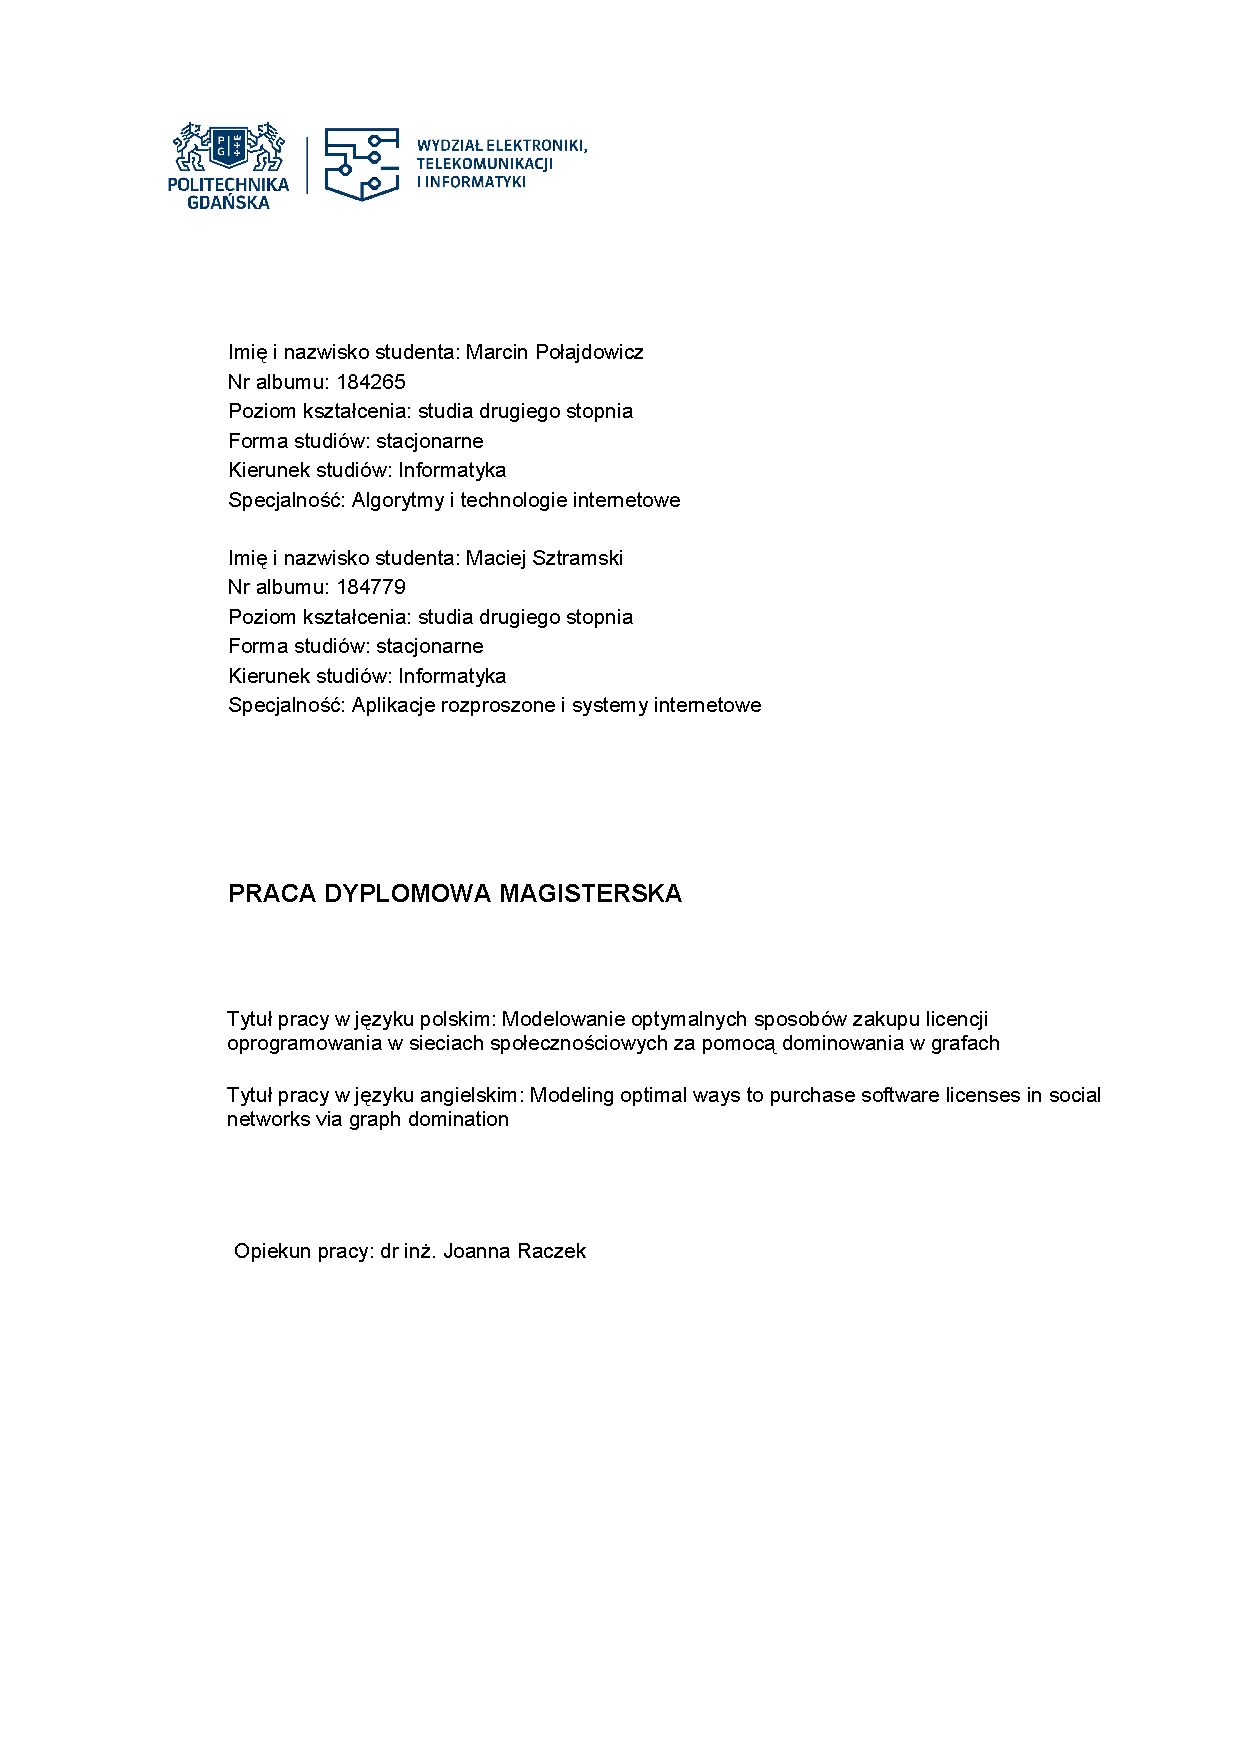
\includepdf[pages=1,pagecommand={}]{assets/titlepage.pdf}

% Include abstracts
\section*{Streszczenie}

Celem niniejszej pracy magisterskiej było opracowanie grafowego modelu optymalizacji zakupu licencji oprogramowania (np. Duolingo Super, Spotify Premium) w sieciach społecznościowych. Problem ten sformułowano jako rozszerzenie klasycznego dominowania (w tym dominowania rzymskiego) w grafach, przy czym uwzględniono praktyczne ograniczenia dotyczące rozmiaru grup licencyjnych oraz struktury kosztów licencji indywidualnych i grupowych.

W pracy przeprowadzono analizę złożoności obliczeniowej problemu, wykazując jego NP-trudność. Zaimplementowano i porównano podejścia algorytmiczne: metody dokładne (ILP/MIP) oraz kilka metod przybliżonych i metaheurystyk (algorytm zachłanny, algorytm genetyczny, przeszukiwanie tabu, symulowane wyżarzanie, algorytm mrówkowy). Badania eksperymentalne wykonano na rzeczywistych ego-sieciach Facebooka oraz na danych syntetycznych (Barabási-Albert, Erdős-Rényi, Watts-Strogatz).

Wyniki pokazują, że metaheurystyki (w szczególności algorytm genetyczny, przeszukiwanie tabu i symulowane wyżarzanie) pozwalają osiągać rozwiązania bliskie optymalnym przy znacznym skróceniu czasu obliczeń względem ILP na większych instancjach. Dodatkowo przeanalizowano wariant dynamiczny, w którym sieć ulega zmianom w czasie, oraz wpływ polityk cenowych i dodatkowych typów planów subskrypcyjnych na optymalne decyzje.

\textbf{Słowa kluczowe:} teoria grafów, optymalizacja kombinatoryczna, dominowanie rzymskie, sieci społecznościowe, heurystyki, metaheurystyki, programowanie całkowitoliczbowe.

\section*{Abstract}

\textbf{PLACHOLDER:} The aim of this master's thesis was to develop a graph-based model for optimizing software license purchases (e.g., Duolingo Super, Spotify Premium) within social networks. The problem was formulated as an extension of classical Roman domination problems in graph theory, incorporating practical constraints such as group-size limitations and specific licensing costs.

This thesis analyzes the computational complexity of the problem, demonstrating its NP-hard nature. Various algorithmic approaches were implemented and compared, including exact methods (Mixed Integer Programming - MIP), heuristics, and advanced metaheuristics (genetic algorithms, Tabu Search, simulated annealing, reinforcement learning). The algorithms were evaluated experimentally on both real-world datasets (from SNAP and NetworkRepository) and synthetic graph models (Barabási–Albert, Erdős–Rényi, Watts–Strogatz).

Experimental results indicate that metaheuristic approaches, particularly genetic algorithms and reinforcement learning, effectively balance solution quality and computational efficiency. The thesis also explores dynamic scenarios in evolving social networks, demonstrating the effectiveness of adaptive algorithms in maintaining cost-efficiency.

Furthermore, the impact of varying pricing strategies and additional subscription types (e.g., Duo, Student plans) on consumer choices was investigated. The applicability of the proposed model in different industries was discussed, along with recommendations for future research directions.

\textbf{Keywords:} graph theory, combinatorial optimization, Roman domination, social networks, metaheuristics, license purchase optimization, NP-hard problems.


% Generate the table of contents (automatically includes chapters and sections)
% Note: To include the bibliography and all references, ensure to compile with Biber or BibTeX after running LaTeX.
\tableofcontents
\listoffigures
\listoftables
\listofalgorithms

\chapter*{Wykaz ważniejszych oznaczeń i skrótów}
\addcontentsline{toc}{chapter}{Wykaz ważniejszych oznaczeń i skrótów}

\section*{Oznaczenia}

\begin{tabular}{@{} l l p{0.7\textwidth} @{}}
    $G=(V,E)$    & -- & graf relacji społecznych. \\
    $V,E$        & -- & zbiory wierzchołków i krawędzi. \\
    $N(v),\ N[v]$ & -- & otoczenie wierzchołka $v$ oraz otoczenie domknięte. \\
    $\deg(v)$    & -- & stopień wierzchołka $v$. \\
    $n=|V|,\ m=|E|$ & -- & liczba wierzchołków i krawędzi. \\
    $\Delta$     & -- & maksymalny stopień grafu. \\
    $f:V\to\{0,1,2\}$ & -- & etykietowanie ról (0–odbiorca, 1–indywidualna, 2–grupowa). \\
    $\cost(f)$   & -- & koszt rozwiązania (def. w rozdz.\,\ref{sec:model-formal}). \\
    $\mathcal{L}$ & -- & rodzina typów licencji $\ell_t=(c_t,m_t,k_t)$. \\
    $I,G,R$      & -- & zbiory: licencji indywidualnych, grupowych i odbiorców. \\
    $p$          & -- & względny koszt licencji grupowej $p=c_g/c_1$. \\
\end{tabular}

\section*{Skróty}

\begin{tabular}{@{} l l p{0.7\textwidth} @{}}
    SaaS & -- & Software as a Service. \\
    ILP/MIP & -- & (Mixed) Integer Linear Programming. \\
    GA   & -- & Genetic Algorithm. \\
    SA   & -- & Simulated Annealing. \\
    TS   & -- & Tabu Search. \\
    ACO  & -- & Ant Colony Optimization. \\
    MDS  & -- & Minimum Dominating Set. \\
    RD   & -- & Roman Domination. \\
\end{tabular}



% Include main chapters of the thesis
\chapter{Wprowadzenie}\label{chap:introduction}
\section{Wstęp i motywacja}
W ostatnich latach coraz większe znaczenie zyskują modele subskrypcyjne w sektorze oprogramowania i usług cyfrowych. Zgodnie z indeksem gospodarki subskrypcyjnej rynek ten zwiększył swoją wartość o ponad 400\% od roku 2012 do roku 2021 \cite{subscriptionEconomyIndex}, a w 2024 roku osiągnął przybliżoną wartość blisko 600 miliardów dolarów \cite{subscriptionEconomyPrice2024}.

Model subskrypcyjny zastępuje zakupy jednorazowe. Zapewnia firmom powtarzalne przychody, a użytkownikom ciągły dostęp do usług. Wiele popularnych platform, w tym aplikacje edukacyjne, serwisy streamingowe czy oprogramowanie w modelu Software as a Service (SaaS), opiera się na modelu subskrypcyjnym. Serwisy streamingowe, takie jak Spotify i Netflix, oferują plany rodzinne, w których kilka osób współdziela jedną subskrypcję grupową o niższym koszcie jednostkowym niż równoważna liczba subskrypcji indywidualnych. Analogicznie platforma Duolingo udostępnia plan rodzinny Super Duolingo (ang. Duolingo Super Family) \cite{duolingo_family}, który umożliwia grupie użytkowników współdzielenie korzyści subskrypcji premium. Mechanizm ten sprzyja zakupom grupowym i obniża koszt przypadający na użytkownika. W pracy terminy "subskrypcja" i "licencja" traktowane są równoważnie jako czasowe prawa dostępu.

Kontekst społeczny jest kluczowy przy formowaniu grup. Efektywne korzystanie z subskrypcji grupowych wymaga, aby główny posiadacz subskrypcji identyfikował użytkowników zainteresowanych współdzieleniem usługi, np. z powodu podziału kosztów, zbieżnych zainteresowań lub bliskich relacji. Grupy tworzone są głównie wśród krewnych i znajomych, co ułatwia ustanowienie relacji zaufania przy współdzieleniu konta. Dodatkowym czynnikiem jest wygoda: jedna wspólna subskrypcja upraszcza rozliczenia i zapewnia wszystkim członkom grupy jednolity dostęp do usługi. Czynniki społeczne wpływają na strukturę współdzielenia w sieciach użytkowników. Media społecznościowe i komunikatory ułatwiają zawieranie porozumień wśród użytkowników powiązanych. W praktyce użytkownicy koordynują wspólny zakup abonamentu. Sieć powiązań społecznych determinuje, kto z kim może skutecznie współdzielić licencję.

Problem optymalizacyjny polega na wyznaczeniu planu zakupu licencji w grupie powiązanych użytkowników, który minimalizuje łączny koszt dostępu do usługi. Równoważnie, dla danej sieci znajomości i katalogu opcji licencyjnych należy wybrać podzbiór nabywców licencji oraz typy licencji tak, aby wszyscy użytkownicy uzyskali dostęp do usługi przy minimalnym koszcie. Formalnie odpowiada to problemowi pokrycia wierzchołków przez zbiór nabywców licencji tak, aby każdy wierzchołek był objęty licencją lub sąsiadował z wierzchołkiem posiadającym licencję.

Struktura problemu ma ścisłe powiązania z zagadnieniami teorii grafów. Jest ona zbieżna z klasycznym problemem dominowania, ponieważ wybór nabywców licencji grupowych pełni funkcję zbioru dominującego. W obu przypadkach chodzi o to, aby wybrany zestaw wierzchołków pokrywał całą sieć. W rozdziale \ref{chap:roman_domination} wykazano związek z wariantem dominowania rzymskiego. Odniesienia te wspierają cel pracy, którym jest optymalizacja kosztów licencji w społeczności użytkowników.

\section{Przegląd istniejących rozwiązań}

Dotychczas w literaturze brak jest opracowań bezpośrednio analizujących problem optymalnego podziału licencji w sieciach społecznościowych. Zagadnienie minimalizacji kosztów zakupu planów grupowych w sieciach powiązanych użytkowników nie zostało dotąd opisane. Niniejsza praca formułuje i analizuje ten problem w ramach teorii grafów.

Najbliższą analogią jest klasyczne zagadnienie zbioru dominującego, które polega na znalezieniu minimalnego podzbioru wierzchołków, tak by każdy wierzchołek grafu należał do tego zbioru lub był jego sąsiadem. Problem ten jest NP-zupełny, co uzasadnia badania algorytmiczne i heurystyczne~\cite{garey1979}. Szczególne znaczenie w kontekście analizowanego problemu ma dominowanie rzymskie, które zostało szczegółowo opisane w rozdziale \ref{chap:roman_domination}. Koncepcja ta znalazła szerokie zastosowanie i liczne rozszerzenia, m.in. dominowanie włoskie i dominowanie zabezpieczone \cite{Roman2DominationSurvey}.

Model ten jest adekwatny do odwzorowania problemu podziału licencji. Standardowa wersja dominowania rzymskiego zakłada brak ograniczeń co do liczby sąsiadów, których może dominować wierzchołek z etykietą $2$. W praktyce plany subskrypcyjne narzucają limity (np. maksymalnie $6$ osób w planie rodzinnym). Prowadzi to do modelu dominowania z pojemnością, w którym każdy wierzchołek dominujący ma przypisaną wartość $c(v)$ określającą liczbę sąsiadów objętych dominowaniem \cite{CapDom}.

Problem podziału licencji stanowi wariant zagadnienia dominowania w grafach, wykorzystujący idee dominowania rzymskiego oraz jego modyfikacje z ograniczeniami pojemności. Brak specjalistycznych opracowań wskazuje na lukę badawczą. Jednocześnie bogata literatura dotycząca dominowania w grafach dostarcza ugruntowanych narzędzi teoretycznych i algorytmicznych, co pozwala formalnie wykazać NP-trudność badanego problemu oraz zastosować zarówno metody dokładne (np. programowanie całkowitoliczbowe), jak i przybliżone heurystyki, wzorując się na podejściach znanych z teorii dominowania \cite{Roman2DominationSurvey, CapDom}.


\section{Cele i zakres pracy}
Celem niniejszej pracy jest formalizacja i analiza problemu optymalnego zakupu licencji w sieciach społecznościowych, zaproponowanie metod jego rozwiązania oraz weryfikacja przyjętych rozwiązań. W pierwszej kolejności opracowany został model grafowy opisujący powiązania między użytkownikami oraz różne strategie zakupowe wraz z odpowiadającymi im kosztami. Model ten umożliwia zdefiniowanie problemu minimalizacji kosztów jako zadania optymalizacyjnego na grafie. Następnie wykazano ścisły związek z problemem dominowania w grafach. W szczególności pokazano, że dla pewnej klasy modeli licencjonowania zadanie optymalnego doboru subskrypcji jest równoważne znalezieniu minimalnego zbioru dominującego lub rozwiązaniu pokrewnego problemu dominowania rzymskiego. Odwołanie do znanych wyników o dominowaniu obejmuje zarówno aspekty złożoności obliczeniowej, jak i badania nad algorytmami aproksymacyjnymi, co pozwala lepiej zrozumieć trudności badanego problemu oraz zaprojektować efektywne metody jego rozwiązywania.

Zakres pracy obejmuje analizę teoretyczną badanego problemu oraz metody algorytmiczne jego rozwiązania, uzupełnione o eksperymenty obliczeniowe. Rozpatrzone zostały różne modele cenowe licencji, zarówno hipotetyczne, jak i rzeczywiste. Do pierwszej grupy należą warianty nawiązujące do dominowania rzymskiego, w których koszt licencji grupowej stanowi wielokrotność ceny licencji indywidualnej. W drugiej grupie znajdują się modele oparte na rzeczywistych ofertach usług, takich jak Spotify, Netflix i Duolingo, co pozwala weryfikować wyniki w kontekście praktycznych scenariuszy.


Osobno przeanalizowane zostały warianty, w których decyzje zakupowe podejmowane są globalnie (jednocześnie dla całej społeczności), oraz scenariusze dynamiczne. W wersji dynamicznej zakupy realizowane są w kolejnych krokach czasowych, a struktura sieci społecznościowej może się zmieniać (rozszerzanie lub zmniejszanie liczby użytkowników, powstawanie lub zanik relacji). Ze względu na wysoką złożoność obliczeniową problemu przedstawione zostały zarówno metody dokładne, jak i heurystyczne. Metody dokładne gwarantują znalezienie rozwiązania optymalnego, lecz ich czas działania szybko rośnie wraz z rozmiarem grafu. Metody heurystyczne nie gwarantują optymalności, lecz dostarczają rozwiązania dobrej jakości w czasie akceptowalnym obliczeniowo. Celem praktycznym jest wskazanie podejść skutecznych w optymalizacji kosztów subskrypcji w dużych sieciach społecznościowych oraz identyfikacja czynników najsilniej wpływających na wyniki, co zilustrowane jest wynikami eksperymentów.

Podsumowując, w ramach pracy zrealizowane zostały następujące zadania badawcze i implementacyjne:
\begin{itemize}
  \item Sformalizowano model optymalizacji zakupu licencji w sieciach społecznościowych, obejmujący etykietowanie ról $f:V\to\{0,1,2\}$, warunki wykonalności (pokrycie, sąsiedztwo, pojemność) oraz funkcję kosztu.
  \item Wykazano powiązania z dominowaniem rzymskim i sformułowano twierdzenie o równoważności w szczególnym przypadku kosztów i pojemności; omówiono również konsekwencje złożonościowe i aproksymacyjne.
  \item Zaimplementowano i porównano różne metody: ILP (PuLP/CBC), algorytm zachłanny, metaheurystyki (algorytm genetyczny, symulowane wyżarzanie, przeszukiwanie tabu, algorytm mrówkowy).
  \item Opracowano środowisko eksperymentalne dla grafów syntetycznych i ego-sieci platformy Facebook, wraz z pomiarem czasu działania i kosztu.
  \item Przeanalizowano wariant dynamiczny (mutacje grafu) oraz porównano podejścia cold-start i warm-start dla metaheurystyk.
  \item Zbadano wpływ polityk cenowych i typów planów (Individual/Duo/Family) na strukturę rozwiązań i koszt całkowity.
\end{itemize}

\section{Struktura}

Struktura pracy obejmuje dziewięć rozdziałów. Obejmują one część wprowadzającą, w której przedstawiono tło i motywację podjętego zagadnienia, część analityczno-badawczą, zawierającą opis zaproponowanych modeli oraz przeprowadzonych eksperymentów, a także część podsumowującą, w której sformułowano wnioski oraz wskazano możliwe kierunki dalszych badań. Poniżej zaprezentowano opis treści wszystkich rozdziałów, stanowiących kolejne etapy realizacji pracy. \\

\begin{description}
  \item \textbf{Rozdział 1} -- Wprowadzenie. Przedstawia tło problemu, motywację podjęcia tematu oraz znaczenie optymalizacji kosztów w kontekście współdzielenia licencji w sieciach społecznościowych. Określone są cele i zakres pracy oraz jej ogólna struktura.

  \item \textbf{Rozdział 2} -- Model grafowy i analiza problemu. Definiuje reprezentację sieci społecznościowej w postaci grafu oraz formalny opis problemu optymalizacji kosztów. Uwzględnione są przyjęte założenia, definicje pojęć oraz warianty wynikające z odmiennych modeli cenowych i ograniczeń pojemnościowych. Rozdział stanowi podstawę do dalszych rozważań algorytmicznych.

  \item \textbf{Rozdział 3} -- Związek z dominowaniem w grafach. Omawia pojęcie zbiorów dominujących i dominowania rzymskiego, pokazując, w jaki sposób badany problem można interpretować w tych kategoriach. Przedstawione są również aspekty złożoności obliczeniowej, w tym dowód NP-trudności, oraz wynikające z tego konsekwencje dla możliwości projektowania algorytmów.

  \item \textbf{Rozdział 4} -- Dane testowe. Opisuje rodzaje grafów wykorzystanych w eksperymentach: syntetyczne, generowane przy pomocy popularnych modeli (Barabási--Albert, Watts--Strogatz oraz Erdős--Rényi), oraz grafy rzeczywiste pochodzące z repozytoriów badawczych. Uwzględniono także sposób przygotowania instancji testowych oraz narzędzia użyte do wizualizacji sieci.

  \item \textbf{Rozdział 5} -- Metody algorytmiczne optymalizacji kosztów licencji. Rozdział skupia się na części obliczeniowej. Przedstawiona jest formalizacja problemu w postaci programu całkowitoliczbowego oraz opis metod dokładnych, które mogą znaleźć optymalne rozwiązania dla mniejszych instancji. Omówione są także podejścia przybliżone i heurystyczne.

  \item \textbf{Rozdział 6} -- Eksperymenty i analiza wyników. Przedstawia proces oceny algorytmów na przygotowanych danych testowych. Określone są kryteria porównawcze (m.in. czas działania, złożoność obliczeniowa, uzyskane koszty), a następnie zaprezentowane wyniki eksperymentów dla różnych typów grafów i ich skal. Analizowany jest wpływ parametrów algorytmów na efektywność i jakość uzyskiwanych rozwiązań.

  \item \textbf{Rozdział 7} -- Analiza dynamicznej wersji problemu. Rozważany jest scenariusz, w którym zakupy licencji odbywają się sekwencyjnie, a struktura sieci może ulegać zmianie w czasie. Opisane są możliwe adaptacje algorytmów do takiej sytuacji oraz przeprowadzone eksperymenty badające ich skuteczność. Poruszona jest także kwestia stabilności i elastyczności strategii w środowisku dynamicznym.

  \item \textbf{Rozdział 8} -- Rozszerzenia modelu. Omawia dodatkowe aspekty, które mogą wpływać na decyzje optymalizacyjne, takie jak polityki cenowe oraz zróżnicowanie typów licencji. Analizowane są również potencjalne ograniczenia modelu i możliwości jego dalszego uogólnienia.

  \item \textbf{Rozdział 9} -- Podsumowanie i wnioski. Zawiera syntetyczne zestawienie wyników pracy. Wskazuje, w jakim stopniu zrealizowane zostały założone cele, oraz proponuje kierunki dalszych badań, w tym rozwój modeli, udoskonalenia algorytmów oraz badania nad skalowalnością i praktycznymi zastosowaniami. Rozdział ten zamyka całość pracy, odpowiadając na pytania badawcze i wskazując, jak uzyskane rezultaty mogą zostać wykorzystane w praktyce.
\end{description}

\chapter{Model grafowy problemu zakupu licencji}

\section{Reprezentacja grafowa}

Aby formalnie opisać zjawisko współdzielenia licencji, sieć relacji społecznych modelujemy jako graf nieskierowany \( G = (V, E) \). Każdy wierzchołek \( v \in V \) reprezentuje pojedynczego użytkownika, natomiast krawędź \( \{u, v\} \in E \) oznacza, że użytkownicy \( u \) i \( v \) znajdują się w relacji umożliwiającej współdzielenie licencji grupowej. Graf jest nieskierowany, ponieważ zakładamy symetryczność tej relacji: jeśli \( u \) zna \( v \), to również \( v \) zna \( u \).

Przyjmujemy również, że graf \( G \) nie zawiera pętli, tj. \( \{v, v\} \notin E \) dla każdego \( v \in V \), ani krawędzi wielokrotnych - każda para użytkowników może być powiązana co najwyżej jedną krawędzią. Przykład takiej struktury zilustrowano na Rysunku \ref{fig:social_graph}.

\begin{figure}[H]
    \centering
    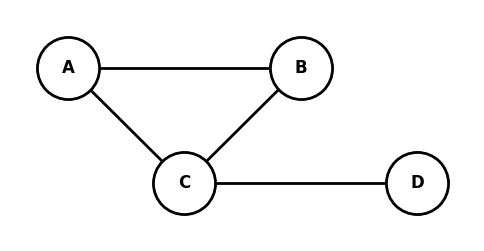
\includegraphics[width=0.5\textwidth]{assets/graphmodelexample.png}
    \caption{Przykładowy graf relacji społecznych między użytkownikami.}
    \label{fig:social_graph}
\end{figure}

Opisana reprezentacja, w której wierzchołki odpowiadają jednostkom, a krawędzie bezpośrednim relacjom umożliwiającym interakcję, jest powszechnie stosowana w analizie sieci społecznościowych \cite{Brandes2004, NETTLETON20131}. Takie ujęcie pozwala formalnie modelować i badać zjawiska zachodzące w społecznościach użytkowników usług cyfrowych.

„W przyjętym modelu zakłada się, że współdzielenie licencji może odbywać się wyłącznie między osobami połączonymi bezpośrednią krawędzią w grafie. Licencja grupowa oznacza w tym kontekście typ umożliwiający współdzielenie dostępu przez właściciela oraz jego bezpośrednich sąsiadów. Oznacza to, że użytkownicy muszą znać się bezpośrednio i mieć wzajemne zaufanie, co jest istotne na przykład w przypadku przekazywania danych logowania lub zapraszania do planu rodzinnego. Relacje pośrednie, w których użytkownicy są powiązani poprzez wspólnych znajomych (np. \( A \sim B \) oraz \( B \sim C \), lecz brak bezpośredniego powiązania \( A \sim C \)), nie są uwzględniane w analizie. Oznacza to, że dla danego grafu \( G = (V, E) \),
w którym \( V \) to zbiór użytkowników, a \( E \subseteq \{ \{u,v\} : u,v \in V, u \neq v \} \) to zbiór relacji znajomości, analizie podlegają wyłącznie relacje bezpośrednie, czyli pary \( \{u, v\} \in E \).
Na przykład w grafie przedstawionym na Rysunku \ref{fig:social_graph}, użytkownicy \( A \) i \( D \) są wprawdzie połączeni za pośrednictwem ścieżki \( A \rightarrow C \rightarrow D \), jednak ponieważ brakuje bezpośredniego połączenia \( \{A,D\} \in E \), to taka relacja nie jest uznawana za podstawę do współdzielenia licencji w tym modelu.
Mimo że w praktyce relacje pośrednie - takie jak ścieżki długości większej niż jeden - mogą sprzyjać tworzeniu grup subskrypcyjnych, w analizie zostały one pominięte w celu uproszczenia problemu.

Graf społecznościowy nie musi być pełny - dopuszcza się dowolną strukturę odpowiadającą rzeczywistym relacjom społecznym. W analizie istotną rolę odgrywa stopień wierzchołków, ponieważ decyduje on o liczbie osób, którym dany użytkownik może udostępnić swoją licencję. Dla wierzchołka \( v \in V \), jego stopień oznaczamy przez \( \deg(v) \), co odpowiada liczbie sąsiadów użytkownika \( v \) w grafie \( G = (V, E) \).

Należy jednak zauważyć, że nawet w przypadku wysokiego stopnia $\deg(v)$, użytkownik niekoniecznie może współdzielić licencję ze wszystkimi swoimi sąsiadami. Ograniczenia techniczne, takie jak limity liczby współużytkowników narzucane przez dostawcę usługi, sprawiają, że liczba osób objętych jedną licencją grupową pozostaje ograniczona. W analizowanym modelu wprowadzamy zatem parametr $k$, oznaczający pojemność licencji grupowej, czyli maksymalną liczbę osób, wliczając w to właściciela, które mogą korzystać z jednej licencji.



\section{Definicja problemu}\label{sec:model-formal}

Optymalizacja kosztu dostępu do usługi wymaga przypisania wszystkim wierzchołkom grafu $G ~=~ (V,~E)$ odpowiednich ról. Każdy użytkownik $v \in V$ może uzyskać dostęp do usługi na trzy sposoby:
\begin{enumerate}
    \item Poprzez wykupienie licencji indywidualnej.
    \item Poprzez wykupienie licencji grupowej.
    \item Jako odbiorca, korzystający z licencji grupowej należącej do innego użytkownika.
\end{enumerate}
Licencja indywidualna zapewnia dostęp wyłącznie jej właścicielowi, natomiast licencja grupowa umożliwia współdzielenie dostępu z maksymalnie $k-1$ sąsiadami w grafie.

Dla przejrzystego i precyzyjnego zdefiniowania modelu wprowadzamy trzy zbiory reprezentujące użytkowników, czyli węzły posiadające własną licencję bądź korzystające z licencji innego węzła:
\begin{itemize}
  \item $I$ - posiadacze licencji indywidualnych;
  \item $G$ - posiadacze licencji grupowych;
  \item $R$ - odbiorcy, którzy sami nie kupują licencji, lecz korzystają z licencji innego użytkownika.
\end{itemize}

Aby formalnie opisać ten podział, wprowadzamy etykietowanie ról $f:V\to\{0,1,2\}$.
Wartość $0$ oznacza węzeł będący odbiorcą, $1$ odpowiada licencji indywidualnej, a $2$ licencji grupowej.
Takie przypisanie nawiązuje do klasycznego problemu dominowania rzymskiego, w którym wierzchołki również otrzymują etykiety z tego samego zbioru wartości.
Odpowiadające zbiory definiujemy jako $I=\{v:f(v)=1\}$, $G=\{v:f(v)=2\}$ oraz $R=V\setminus(I\cup G)$.
Przyjmujemy zbiór dostępnych typów licencji
\begin{equation}
  \mathcal{L} = \{ \ell_t = (c_t, m_t, k_t) \mid t = 1,2,\dots,T \},
  \label{eq:license_family}
\end{equation}
gdzie:
\begin{itemize}
  \item $c_t$ - koszt licencji typu $t$,
  \item $m_t$ — minimalna liczba użytkowników wliczając właściciela,
  \item $k_t$ — maksymalna liczba użytkowników wliczając właściciela,
  \item $T$ — całkowita liczba dostępnych typów licencji.
\end{itemize}
W podstawowym wariancie rozważanym w tym rozdziale zakładamy, że zbiór $\mathcal{L}$ opisany we wzorze~(\ref{eq:license_family}) obejmuje wyłącznie dwa typy licencji: indywidualną oraz jedną grupową, a zatem przyjęte jest $T = 2$. Model ten nie przewiduje sytuacji z wieloma rodzajami planów grupowych (np. Duo, Family), lecz ogranicza się do najprostszego przypadku odpowiadającego rozwiązaniom takim jak w Duolingo.

\paragraph{Warunki wykonalności.}
Spełnienie rozwiązania wymaga, aby dla etykietowania $f:V\to\{0,1,2\}$ zachodziły następujące warunki:
\begin{enumerate}
  \item Pokrycie: Każdy użytkownik $v \in V$ musi mieć dostęp do usługi, tj. $f(v)\in\{1,2\}$ lub istnieje sąsiad $u\in N(v)$ taki, że $f(u)=2$ i $v$ jest przypisany do grupy $u$.
  \item Sąsiedztwo: Odbiorca $v\in R$ może być przypisany tylko do właściciela $u\in G$ z $\{u,v\}\in E$.
  \item Pojemność: Liczba użytkowników przypisanych do właściciela $u\in G$ (wraz z nim samym) musi spełniać $m \le 1+|R_u| \le k$, gdzie $R_u$ oznacza zbiór odbiorców korzystających z licencji $u$.
\end{enumerate}


\paragraph{Funkcja kosztu.}
W wariancie podstawowym, w którym $T=2$, całkowity koszt rozwiązania wyraża się zależnością:
\begin{equation}
  \cost(f) = |I|\cdot c_i + |G|\cdot c_g ,
  \label{eq:cost_function}
\end{equation}
gdzie:
\begin{itemize}
  \item $I$ - zbiór użytkowników z licencją indywidualną,
  \item $G$ - zbiór użytkowników z licencją grupową,
  \item $c_i$ - koszt licencji indywidualnej,
  \item $c_g$ - koszt licencji grupowej.
\end{itemize}

\paragraph{Cel optymalizacji.}
Celem problemu jest minimalizacja funkcji kosztu~(\ref{eq:cost_function}) dla danego grafu $G=(V,E)$, przy spełnieniu wszystkich istotnych warunków wykonalności.


% Odpowiadający problem decyzyjny polega na sprawdzeniu, czy istnieje taki wybór zbiorów $I$ i $G$, że spełnione są wszystkie warunki oraz zachodzi nierówność:
% \[
% |I| + p \cdot |G| \leq K,
% \]
% dla danego ograniczenia kosztowego $K$.

\section{Koszty i ograniczenia}

\subsection{Ograniczenia techniczne i społeczne współdzielenia licencji}

Kluczowymi parametrami modelu są minimalna oraz maksymalna liczba osób, które mogą współdzielić jedną licencję grupową. Maksymalny rozmiar grupy oznaczamy przez $k$ i wliczamy do niego także użytkownika nabywającego licencję. Parametr $k$ jest zwykle narzucany przez dostawcę usługi. Przykładowo, plan rodzinny Spotify Premium pozwala na korzystanie maksymalnie sześciu osobom (właściciel + pięć członków rodziny), co odpowiada wartości $k=6$.

Analogicznie wprowadzamy parametr $m$, który określa minimalną liczbę osób niezbędnych do utworzenia grupy. Oznacza to, że licencja grupowa jest ważna tylko wtedy, gdy zostanie wykorzystana przez co najmniej $m$ osób (łącznie z właścicielem). Przykładem jest tzw. plan „Duo”, w którym licencję mogą współdzielić dokładnie dwie osoby ($m=2, k=2$). W innych przypadkach $m$ może przyjmować wartości mniejsze niż $k$, np. $m=2, k=6$ dla planów rodzinnych.

W analizie przyjmujemy $m$ oraz $k$ jako zmienne parametry. Nawet jeśli użytkownik posiada wielu znajomych (czyli ma wysoki stopień w grafie), ograniczenie $k$ sprawia, że może objąć współdzieleniem tylko określoną maksymalną liczbę osób, natomiast ograniczenie $m$ wymusza, by grupy nie były zbyt małe. Parametry te modelują zarówno ograniczenia techniczne narzucane przez dostawców usług, jak i czynniki społeczne, takie jak opłacalność czy gotowość do współdzielenia subskrypcji. W konsekwencji grupy współdzielenia odwzorowują typowe sytuacje, w których w praktyce licencje grupowe są wykorzystywane.


% \subsection{Struktura kosztów i modele cenowe}

% Przyjmujemy, że koszt licencji indywidualnej wynosi $1$ jednostkę, natomiast koszt licencji grupowej oznaczamy przez $p$. W rzeczywistych ofertach wartość $p$ różni się w zależności od usługi, lecz zazwyczaj jest mniejsza niż suma kosztów indywidualnych licencji dla wszystkich użytkowników planu, co stanowi zachętę do współdzielenia. W szczególności interesujące są przypadki, gdy $p < k$, ponieważ wtedy koszt jednostkowy w planie grupowym, równy $p/k$, jest niższy niż $1$.

% Jeżeli natomiast $p = k$, oznaczałoby to brak korzyści ze współdzielenia - koszt na osobę byłby identyczny jak w przypadku zakupu licencji indywidualnej. W praktyce jednak zazwyczaj zachodzi $p < k$, a często nawet $p \ll k$, co czyni współdzielenie ekonomicznie korzystnym.

% Do zilustrowania różnych scenariuszy rozważane będą miedzy innymi poniższe modele cenowe:
% \begin{enumerate}
%     \item \textbf{Model A}: $p=2$, $k=5$ - licencja grupowa dwukrotnie droższa od indywidualnej, obejmująca pięć osoby,
%     \item \textbf{Model B}: $p=3$, $k=5$ - licencja grupowa trzykrotnie droższa od indywidualnej, również obejmująca pięć osób.
% \end{enumerate}
% Zarówno model A jak i model B reprezentują rzeczywisty rozmiar ilości osób mogących korzystać z jednej zakupionej licencji grupowej. Istotną różnicą jest tutaj cena obu tych przypadków. Interesujący może być wpływ ceny na ilość występowania zakupionych licencji indywidualnych oraz grupowych w porównaniu modeli o różnych wartości obu tych licencji.

\subsection{Struktura kosztów i modele cenowe}

W analizowanym problemie istotnym elementem jest sposób odwzorowania polityki cenowej dostawców usług.
Różne plany subskrypcyjne charakteryzują się nie tylko innym kosztem, ale również odmiennym zakresem liczby użytkowników $k$, którzy mogą korzystać z jednej licencji.
Dodatkowo wprowadzane jest ograniczenie dolne $m$, które definiuje minimalną liczbę użytkowników planu.
Mimo że w rzeczywistości takie ograniczenia nie są formalnie narzucane, w prezentowanym modelu pełnią ważną rolę, gdyż odzwierciedlają ekonomiczny sens wyboru licencji grupowych.
W praktyce bowiem korzystanie z planu grupowego przez jedną osobę jest nieopłacalne.
Przykładowo, dla planów typu Duo czy Family naturalne jest przyjęcie $m=2$, mimo że technicznie możliwe byłoby używanie takiej subskrypcji w pojedynkę.
Rodzinę typów licencji zdefiniowaną we wzorze~\eqref{eq:license_family} stosujemy tutaj do opisu struktury kosztów i ograniczeń dostępnych planów.
W testach syntetycznych wartości parametrów licencji dobierane są eksperymentalnie, co pozwala badać zachowanie algorytmów w różnych wariantach cenowych i strukturalnych.
W testach na danych rzeczywistych wykorzystywane są faktyczne ceny subskrypcji.
Dla wariantu teoretycznego odpowiadającego dominacji rzymskiej koszty normalizowane są względem licencji indywidualnej, co umożliwia powiązanie modelu z klasycznymi zagadnieniami teorii grafów.
Przykłady zestawiono w~Tabeli~\ref{tab:license_models_real}.


\begin{table}[h!]
\centering
\caption{Przykładowe modele licencji dla usług rzeczywistych i modelu teoretycznego}
\begin{tabular}{lccc}
\hline
\textbf{Typ licencji} & \textbf{Koszt $c_t$} & \textbf{Min $m_t$} & \textbf{Max $k_t$} \\
\hline
\multicolumn{4}{c}{\textit{Spotify (ceny w PLN)}} \\
Individual & 23,99 & 1 & 1 \\
Duo        & 30,99 & 2 & 2 \\
Family     & 37,99 & 2 & 6 \\
\hline
\multicolumn{4}{c}{\textit{Netflix (ceny w PLN)}} \\
Basic       & 33,00 & 1 & 1 \\
Standard    & 49,00 & 1 & 2 \\
Premium     & 67,00 & 1 & 4 \\
\hline
\multicolumn{4}{c}{\textit{Duolingo Super (ceny w PLN)}} \\
Individual & 13,99 & 1 & 1 \\
Family     & 29,17 & 2 & 6 \\
\hline
\multicolumn{4}{c}{\textit{Model teoretyczny (koszty znormalizowane)}} \\
Solo       & 1,0   & 1 & 1 \\
Group      & 2,0   & 2 & 999999 \\
\hline
\label{tab:license_models_real}
\end{tabular}

Źródło: opracowanie własne modelu teoretycznego oraz \cite{spotify_price2024}, \cite{spotify_price2025}, \cite{duolingo_app2024}.

\end{table}


W przypadku usług rzeczywistych koszty planów grupowych są znacznie niższe niż suma odpowiadających im licencji indywidualnych. Na przykład plan Spotify Family pozwala na współdzielenie subskrypcji przez maksymalnie sześć osób przy koszcie $37{,}99$ PLN, co czyni go zdecydowanie bardziej opłacalnym od planu indywidualnego ($23{,}99$ PLN). Podobna sytuacja występuje w przypadku Duolingo Super Family.

W modelu teoretycznym opartym na dominacji rzymskiej koszty są podane w jednostkach względnych. Licencja indywidualna ma koszt $1.0$, a licencja grupowa koszt $2.0$, co odpowiada klasycznemu przypisaniu wag w problemie dominacji rzymskiej. W ramach przeprowadzanych eksperymentów etykieta „2” będzie zmieniała swoją wartość jako wielokrotność kosztu ceny indywidualnej, co pozwala na analizę różnych wariantów tego zagadnienia.


% \subsection{Zakup jednoczesny i sekwencyjny}

% W podstawowej wersji problemu zakłada się, że decyzje zakupowe wszystkich użytkowników są podejmowane jednocześnie, co umożliwia globalną optymalizację. W praktyce jednak proces współdzielenia często przebiega dynamicznie. Najpierw pewne grupy użytkowników kupują licencje indywidualnie, a dopiero później tworzą grupy współdzielenia.

% Taki dynamiczny scenariusz można modelować jako proces wieloetapowy, w którym w kolejnych krokach następuje przydział użytkowników do nowych licencji. Warto zauważyć, że rozwiązanie optymalne przy jednoczesnym zakupie może być trudne do osiągnięcia w procesie sekwencyjnym. Decyzje podejmowane wcześniej mogą ograniczać dostępne opcje w kolejnych etapach.

% W pracy omówione zostaną wyzwania związane z rozwiązaniami sekwencyjnymi, takie jak stabilność struktur współdzielenia czy mechanizmy motywujące do współpracy. Główny nacisk kładziony jest jednak na analizę wariantu jednoczesnego, który umożliwia zastosowanie klasycznych narzędzi teorii grafów i optymalizacji dyskretnej, oraz stanowi punkt odniesienia dla bardziej złożonych scenariuszy dynamicznych.

\subsection{Zakup jednoczesny i sekwencyjny}

W najprostszym wariancie zakłada się, że wszystkie decyzje zakupowe zapadają w tym samym momencie. Umożliwia to globalną optymalizację i stanowi punkt odniesienia dla analiz teoretycznych. W praktyce jednak proces współdzielenia licencji jest bardziej dynamiczny. Użytkownicy dołączają do planów w różnych chwilach, część początkowo wybiera licencje indywidualne, a dopiero później postanawia zakupić subskrypcję grupową. Takie zmiany licencji mogą również wynikać z równoczesnej zmiany i ewolucji sieć społecznościowej w czasie rzeczywistym. Relacje znajomości mogą zanikać, powstawać mogą nowe połączenia, a liczba aktywnych użytkowników zmienia się w czasie.

Takie sytuacje można modelować jako proces sekwencyjny, w którym w kolejnych krokach przydzielane są nowe licencje przy uwzględnieniu bieżącej struktury grafu. Prowadzi to do odmiennych trudności niż w przypadku wariantu uproszczonego, czyli jednoczesnego. Rozwiązanie optymalne globalnie może okazać się nieosiągalne, ponieważ wcześniejsze decyzje oraz zmiany w strukturze sieci ograniczają przestrzeń dostępnych opcji w późniejszych etapach.

W pracy przeanalizowane zostały konsekwencje tego typu dynamicznych zmian takie jak stabilność i trwałość powstałych grup, wpływ zmian w grafie na opłacalność wcześniejszych decyzji, a także mechanizmy sprzyjające koordynacji i adaptacji użytkowników. Mimo że główny nacisk położony jest na wariant jednoczesny, wariant sekwencyjny stanowi istotne rozszerzenie modelu i lepiej odzwierciedla rzeczywiste warunki funkcjonowania sieci społecznościowych.

\chapter{Związek z dominowaniem w grafach}
\label{chap:roman_domination}

W niniejszym rozdziale przedstawiono teoretyczne podstawy problemu licencjonowania oprogramowania poprzez przegląd teorii dominowania w grafach. Rozdział zawiera definicje podstawowych pojęć, wprowadza formalizację problemu licencjonowania jako wariantu dominowania rzymskiego oraz analizuje złożoność obliczeniową zagadnienia. Całość stanowi teoretyczne uzasadnienie dla metod algorytmicznych opisanych w dalszej części pracy.

\section{Dominowanie -- podstawowe definicje}
Problematyka dominowania w grafach jest dobrze zbadana i szeroko opisana w literaturze~\cite{haynes1998domination}.
W szczególności znane są klasyczne definicje zbioru dominującego oraz liczby dominowania, które stanowią punkt odniesienia dla dalszych analiz.
Niech $G=(V,E)$ będzie grafem nieskierowanym.
Zbiorem dominującym jest podzbiór $D \subseteq V$ taki, że każdy wierzchołek spoza $D$ ma co najmniej jednego sąsiada w $D$:
\begin{equation}
  \forall v \in V \setminus D \;\; \exists\, u \in D : \{u,v\} \in E ,
  \label{eq:dominating_set_def}
\end{equation}
gdzie:
\begin{itemize}
  \item $V$ - zbiór wierzchołków grafu,
  \item $E$ - zbiór krawędzi grafu,
  \item $D \subseteq V$ - zbiór dominujący,
  \item $u,v \in V$ - wierzchołki grafu,
  \item $\{u,v\}\in E$ - krawędź łącząca wierzchołki $u$ i $v$.
\end{itemize}


Najmniejszą moc zbioru dominującego oznaczamy symbolem $\gamma(G)$ i nazywamy liczbą dominowania:
\begin{equation}
  \gamma(G) = \min \{\, |D| : D \subseteq V \,\},
  \label{eq:domination_number}
\end{equation}
gdzie:
\begin{itemize}
  \item $\gamma(G)$ - liczba dominowania grafu $G$,
  \item $D$ - zbiór dominujący w grafie $G$,
  \item $V$ - zbiór wierzchołków grafu,
  \item $|D|$ - moc zbioru $D$.
\end{itemize}



Z punktu widzenia rozważanego problemu zakupu licencji, podstawowe założenie jest następujące:
jeśli potraktujemy osoby kupujące licencje jako zbiór \(D\), a krawędzie grafu jako relacje
umożliwiające udostępnianie licencji, wówczas warunek dominowania opisany równaniem~(\ref{eq:dominating_set_def}) określa sytuację,
w której każdy użytkownik spoza $D$ ma znajomego w~$D$, a zatem uzyskuje dostęp do usługi.
Gdyby wszystkie licencje były identyczne i pozwalały obsłużyć dowolną liczbę sąsiadów,
minimalizacja kosztu sprowadzałaby się do wyznaczenia liczby dominowania~(\ref{eq:domination_number}).
W praktyce jednak występują różne typy licencji oraz limity
współużytkowników, co czyni problem znacznie bardziej złożonym.

Należy zauważyć, że najmniejszy zbiór dominujący nie musi być jednoznaczny.
W niektórych przypadkach można w grafie znaleźć kilka różnych najmniejszych zbiorów dominujących.
Wynika to bezpośrednio z definicji liczby dominowania~(\ref{eq:domination_number}),
która określa jedynie minimalną moc zbioru dominującego, a nie jego unikalność.
Często graf ma wiele zbiorów dominujących o rozmiarze równym $\gamma(G)$,
jak na rysunku~\ref{fig:dominatingexample}, gdzie trzy zbiory są minimalne względem inkluzji, ale tylko dwa są najmniejsze.
Problem znajdowania $\gamma(G)$ jest jednak dobrze określony i należy do klasy problemów NP-trudnych. Jego wersja decyzyjna sformułowana jest następująco: dla zadanego grafu $G$ oraz liczby całkowitej $k$ pytamy, czy istnieje zbiór dominujący o rozmiarze co najwyżej $k$. Jest to klasyczny problem NP-zupełny \cite{wikiDominatingSet, POUREIDI2023106363, PANDA2023337}. Oznacza to, że najprawdopodobniej (przy założeniu $P \neq NP$) nie istnieje algorytm wielomianowy rozwiązujący ten problem w ogólności. W praktyce stosuje się zatem algorytmy przybliżone lub ogranicza analizę do specjalnych klas grafów, dla których problem staje się prostszy. Znane są między innymi efektywne algorytmy zachłanne, które zapewniają rozwiązanie przybliżone z gwarantowanym współczynnikiem. Przykładem jest prosty algorytm zachłanny wybierający kolejno wierzchołki do zbioru dominującego, osiągający przybliżenie rzędu $O(\ln n)$.


\begin{figure}[H]
  \centering
  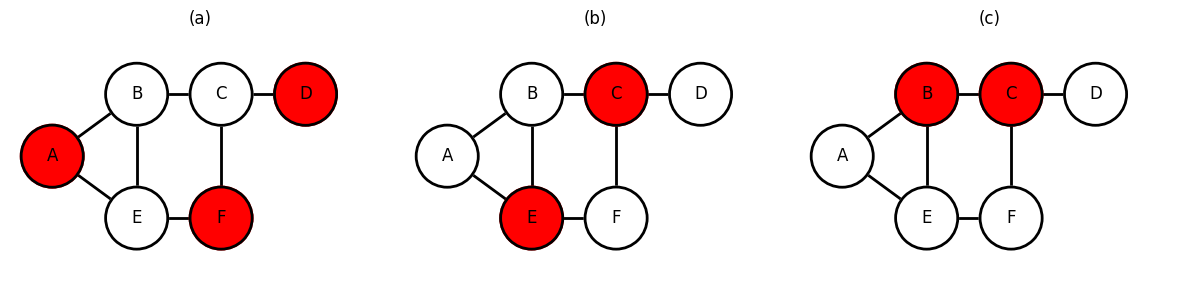
\includegraphics[width=1\textwidth]{assets/dominating-set-example.png}
  \caption[Przykładowe zbiory dominujące]{%
    Przykładowe zbiory dominujące (wyróżnione na czerwono).
    \textbf{(a)}~Minimalny zbiór dominujący o mocy~3.
    \textbf{(b)}-\textbf{(c)}~Dwa różne minimalne i najmniejsze zbiory dominujące, gdzie
    \(\gamma(G)=2\).  Każdy wierzchołek nieczerwony ma sąsiada czerwonego.
  }
  \label{fig:dominatingexample}
\end{figure}

W ogólności nie można poprawić granicy aproksymacji rzędu logarytmicznego. Problem zbioru dominującego jest APX-trudny, a dokładniej log-APX-zupełny \cite{POUREIDI2023106363}. Co więcej, nawet na bardzo ograniczonych grafach, np. grafach o maksymalnym stopniu 3 (grafy kubiczne), problem pozostaje NP-trudny i APX-zupełny \cite{ALIMONTI2000123}. Berman i Fujito (1999) wykazali m.in. NP-trudność pewnych wariantów dominowania w grafach o ograniczonym stopniu \cite{BermanFujitoThreeDegree}, co potwierdza, że zasadnicza trudność problemu dominowania jest obecna już w stosunkowo prostych strukturach.


\section{Dominowanie rzymskie a licencje grupowe}

Dominowanie rzymskie to wariant problemu dominowania, w którym każdemu wierzchołkowi przypisuje się jedną z trzech wartości: 0, 1 lub 2. Wierzchołek o wartości 1 dominuje wyłącznie samego siebie, natomiast wierzchołek o wartości 2 dominuje zarówno siebie, jak i wszystkich swoich sąsiadów. Wymaga się przy tym, aby każdy wierzchołek o wartości 0 był sąsiadem co najmniej jednego wierzchołka oznaczonego wartością 2. Formalnie, funkcja dominowania rzymskiego na grafie $G=(V,E)$ to funkcja $f: V \to \{0,1,2\},$ spełniająca warunek, że dla każdego wierzchołka $v$ z $f(v) = 0$ istnieje sąsiad $u \in V$ taki, że $f(u) = 2$ \cite{Favaron2009}. Minimalizacja sumy wartości $f(v)$ po wszystkich $v \in V$ prowadzi do zdefiniowania tzw. liczby dominowania rzymskiego grafu, oznaczanej $\gamma_R(G)$.

Terminologia i metafora związana z dominowaniem rzymskim wywodzą się z legendy o obronie granic imperium rzymskiego. Zakładano w niej, że w każdej osadzie można umieścić pewną liczbę jednostek wojskowych. Osada z dwiema jednostkami była w stanie bronić się samodzielnie i jednocześnie wysłać wsparcie do sąsiedniej osady. Osada z jedną jednostką broniła wyłącznie siebie, a miejscowości pozbawione jednostek militarnych wymagały ochrony z zewnątrz. W tej metaforze graf reprezentuje system osad i połączeń między nimi, a etykiety 0, 1 i 2 odpowiadają decyzjom o rozmieszczeniu wojsk. Koncepcję dominowania rzymskiego wprowadzili do teorii grafów Cockayne i współpracownicy w 2004 roku \cite{Cockayne2004}.


W kontekście problemu optymalnego zakupu licencji w grafach reprezentujących sieci społecznościowe interpretacja jest bezpośrednia. Wartość $f(v)=2$ odpowiada użytkownikowi $v$, który nabywa licencję grupową i zapewnia dostęp zarówno sobie, jak i co najmniej jednemu ze swoich sąsiadów. Wartość $f(v)=1$ oznacza użytkownika posiadającego licencję indywidualną, pokrywającą wyłącznie jego samego. Natomiast $f(v)=0$ reprezentuje użytkownika bez własnej licencji, który musi polegać na pokryciu przez sąsiada z wartością 2. Warunek dominowania rzymskiego, zgodnie z którym każdy wierzchołek z etykietą 0 ma sąsiada z etykietą 2, gwarantuje dokładnie to, co w naszym modelu jest wymagane: każdy użytkownik bez licencji ma znajomego z licencją grupową, który może podzielić się z nim dostępem. W ten sposób każda funkcja $f:V \to \{0,1,2\}$ spełniająca warunki dominowania rzymskiego wyznacza dopuszczalną strategię licencyjną w rozważanej sieci.


Waga funkcji dominowania rzymskiego definiowana jest jako $w(f) = \sum_{v \in V} f(v)$, czyli suma przypisanych wartości. Liczba dominowania rzymskiego $\gamma_R(G)$ to najmniejsza możliwa waga funkcji dominowania rzymskiego dla grafu $G$. Jeśli przyjmiemy, że koszt licencji indywidualnej wynosi 1, a grupowej 2, to minimalizacja kosztu w naszym problemie pokrywa się z zagadnieniem znalezienia funkcji dominowania rzymskiego o najmniejszej wadze. Cel minimalizacji całkowitego kosztu $C = |I| + 2|H|$ jest równoważny minimalizacji $w(f)$, gdy $|I|$ utożsamimy z liczbą wierzchołków o etykiecie 1, a $|H|$ z liczbą wierzchołków o etykiecie 2. Należy jednak podkreślić, że pełna równoważność z dominowaniem rzymskim zachodzi tylko wtedy, gdy liczba sąsiadów dowolnego wierzchołka nie przekracza maksymalnej liczby użytkowników dopuszczonych w planie grupowym. Jak wspomniano wcześniej przy omawianiu parametrów $m$ i $k$, nasze ujęcie wprowadza dodatkowe ograniczenie pojemności -- wierzchołek dla którego funkcja $f$ przyjmuje wartość 2 może pokrywać jedynie ograniczoną liczbę sąsiadów. Problem optymalnego zakupu licencji jest więc uogólnieniem dominowania rzymskiego, dostosowanym do praktycznych limitów występujących w planach subskrypcyjnych.

W przypadku innych modeli cenowych, dominowanie rzymskie stanowi nadal użyteczną metaforę, choć nie oddaje w sposób wystarczający struktury kosztów. 
Stosunek kosztu licencji grupowej do indywidualnej oznaczamy przez $p_r = c_g / c_i$. W klasycznym dominowaniu rzymskim przyjmuje się, że $p_r=2$, co odpowiada sytuacji, w której licencja grupowa kosztuje dokładnie dwukrotnie więcej niż indywidualna.
Gdy $p_r \neq 2$, możemy rozważyć ogólniejsze przypisania wag, w których etykieta odpowiada rzeczywistemu kosztowi planu. Przykładowo, gdy $p_r=3$, to licencja grupowa ma koszt równy trzem jednostkom, co nie mieści się w klasycznym schemacie $\{0,1,2\}$. W literaturze zaproponowano rozszerzenia pozwalające modelować podobone sytuacje, m.in. $k$-dominowanie rzymskie, gdzie dopuszcza się wartości $\{0,1,\dots,k\}$ \cite{CHAUDHARY2024301}, czy też dominowanie rzymskie z wagami \cite{Ghaffari2020}. Warianty te pozwalają odwzorować przypadki, w których dostępne są plany o różnych kosztach i różnej pojemności, np. licencja droższa, ale umożliwiająca współdzielenie w większej grupie. W tym sensie uogólnienia dominowania rzymskiego są bliższe rzeczywistemu problemowi optymalizacji kosztów licencji niż klasyczna wersja ograniczona do wartości 0, 1 i 2.

Na potrzeby tej pracy nie jest jednak konieczne wchodzenie w szczegółowe odmiany dominowania rzymskiego. Wystarczy zauważyć, że w analizowanym modelu schemat pozostaje taki sam jak w klasycznej wersji, a jedyną różnicą jest koszt przypisywany wierzchołkom o etykiecie $2$. W zależności od przyjętego modelu cenowego wartość ta może wynosić np. $p_r=1.5$, $p_r=2.5$ lub $p_r=3$. Konstrukcja funkcji dominowania rzymskiego oraz sam podział na etykiety $\{0,1,2\}$ nie ulega zmianie. Innymi słowy, dominowanie rzymskie dostarcza prostego i intuicyjnego opisu sytuacji.

Prosty przykład zastosowania dominowania rzymskiego można przedstawić na grafie typu gwiazda. Centralny wierzchołek $A$ jest połączony z liśćmi $B, C, D, E$. Najlepszą strategią jest, aby $A$ wykupił licencję grupową i udostępnił ją wszystkim swoim sąsiadom. W modelu oznacza to $f(A)=2$, a dla każdego liścia $f(B)=f(C)=f(D)=f(E)=0$. Warunek dominowania rzymskiego jest spełniony, ponieważ każdy liść, dla którego $f=0$, ma sąsiada $A$ z $f=2$. Waga funkcji wynosi wówczas $w(f)=2$ - odpowiada to kosztowi jednej licencji grupowej obsługującej całą pięcioosobową grupę.

Dla porównania można rozważyć inne strategie. Gdyby każdy wierzchołek nabył licencję indywidualną, wówczas $w(f)=5$, co odpowiada kosztowi pięciu licencji indywidualnych. Jeśli centralny wierzchołek nabyłby wyłącznie licencję indywidualną ($f(A)=1$), a liście pozostałyby bez dostępu ($f(B)=f(C)=f(D)=f(E)=0$), warunek nie byłby spełniony, ponieważ żaden liść nie miałby sąsiada przyjmującego dla funkcji $f$ wartość 2.

Rysunek~\ref{fig:romandomatinonstarexamepl} ilustruje przykład i pokazuje, jak dominowanie rzymskie wskazuje optymalny wybór wierzchołka centralnego jako posiadacza licencji grupowej. W większych grafach liczba kandydatów do roli posiadaczy licencji grupowych rośnie, a ich dobór prowadzi do problemu optymalizacji funkcji dominowania rzymskiego.


\begin{figure}[H]
  \centering
  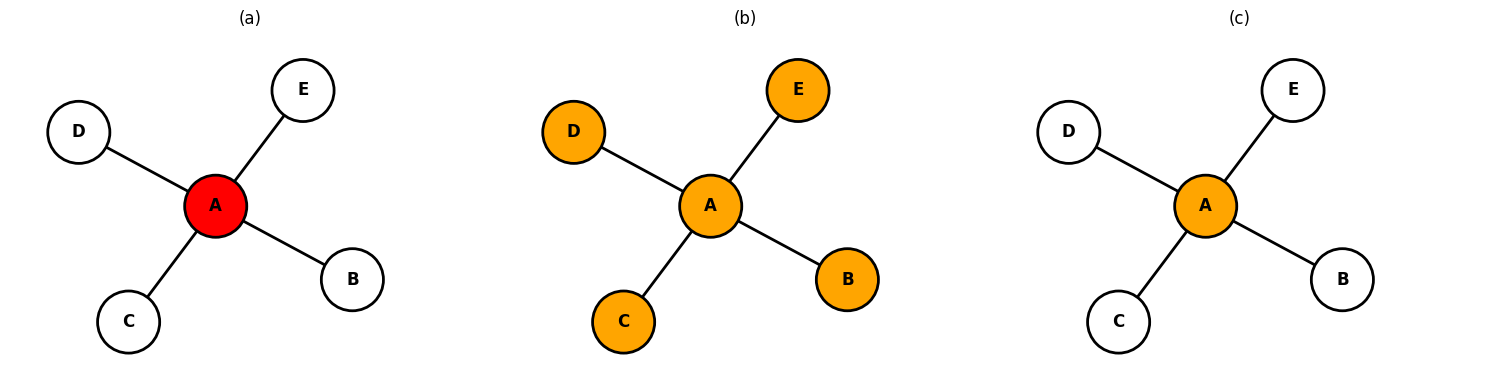
\includegraphics[width=1\textwidth]{assets/stars.png}
  \caption{
  Przykład dominowania rzymskiego na grafie typu gwiazda.  
  Kolory: biały = $f(v)=0$, pomarańczowy = $f(v)=1$, czerwony = $f(v)=2$.
    \textbf{(a)}~Przypisanie optymalne ($w(f)=2$).
    \textbf{(b)}~$f(A)=f(B)=f(C)=f(D)=f(E)=1$ ($w(f)=5$).
    \textbf{(c)}~$f(A)=1$, liście $f(B)=f(C)=f(D)=f(E)=0$ (niespełniony warunek).
  }
  \label{fig:romandomatinonstarexamepl}
\end{figure}


\section{Złożoność obliczeniowa problemu}

Dokładne dowody z zakresu złożoności obliczeniowej znajdują się w literaturze; wykazano NP-zupełność problemu dominowania rzymskiego m.in. przez redukcję z problemu pokrycia wierzchołków lub zbioru dominującego \cite{chambers2009}. W kontekście naszego modelu oznacza to, że optymalne wyznaczenie użytkowników kupujących poszczególne licencje jest obliczeniowo trudne dla dużych sieci. Innymi słowy, nie istnieje znany algorytm wielomianowy, który gwarantowałby znalezienie rozwiązania minimalnego kosztu dla dowolnej struktury grafu znajomości - w najgorszym przypadku liczba kombinacji rośnie wykładniczo wraz z liczbą wierzchołków.

Konsekwencją NP-trudności jest także brak prostego schematu aproksymacyjnego dla problemu minimalizacji kosztów licencji. Ponieważ problem dominowania (minimalnego zbioru dominującego) jest APX-zupełny (dla konkretnych rodzajów grafów) \cite{POUREIDI2023106363}, nie ma wielomianowego schematu aproksymacji (PTAS) gwarantującego dobre przybliżenie. Dla naszego problemu, który uogólnia dominowanie, obowiązują podobne ograniczenia; w najgorszym przypadku nie uzyska się w czasie wielomianowym przybliżenia lepszego niż rzędu $O(\ln n)$. Proste heurystyki zachłanne mogą jednak dawać przyzwoite wyniki. Przykładowo heurystyka wybierająca iteracyjnie wierzchołek pokrywający najwięcej niepokrytych sąsiadów (z przypisaniem licencji grupowej) realizuje algorytm zachłanny i osiąga współczynnik co najwyżej $2+\ln \Delta$, gdzie $\Delta$ to maksymalny stopień grafu \cite{Kuhn2012NetworkAlgorithms}. W najgorszym przypadku jest to $O(\ln n)$, natomiast w praktyce wyniki bywają lepsze od tej granicy. Problem pozostaje trudny także dla grafów o niewielkich stopniach; dla grafów o stopniu co najwyżej cztery wyznaczenie najmniejszego zbioru dominującego jest APX-zupełne \cite{ALIMONTI2000123,POUREIDI2023106363}.
Wynika stąd, że ograniczenie maksymalnej liczby sąsiadów nie upraszcza problemu do trywialnego. Nawet w sieciach o małym stopniu optymalny przydział do licencji grupowych może wymagać złożonych obliczeń.

W dalszej części pracy nacisk położono na podejścia algorytmiczne uwzględniające tę złożoność. Przyjęto podejście dwutorowe: (a) zastosowanie metod dokładnych dla umiarkowanych rozmiarów sieci oraz (b) projektowanie i analizę algorytmów heurystycznych dostarczających dobre rozwiązania dla większych sieci. W literaturze można już znaleźć próby wykorzystania technik optymalizacyjnych do problemu dominowania; przykładem jest praca Parra Inza i współautorów \cite{PARRAINZA2024926}, w której zagadnienie sformułowano jako ILP i uzupełniono heurystykami naprawczymi. Tego typu konstrukcję można zaadaptować do omawianego problemu, wprowadzając zmienne decyzyjne wskazujące wybór typu licencji dla każdego użytkownika oraz odpowiednie ograniczenia. Algorytmy zachłanne, metody lokalnego przeszukiwania oraz metaheurystyki, np. algorytmy genetyczne czy symulowane wyżarzanie, pozwalają szybko przeszukiwać przestrzeń możliwych konfiguracji licencji.

\section{Podsumowanie}

W niniejszym rozdziale przedstawiono teoretyczne podstawy problemu licencjonowania oprogramowania w kontekście teorii dominowania w grafach. Kluczowym wnioskiem jest identyfikacja problemu jako wariantu dominowania rzymskiego, gdzie węzły mogą przyjmować różne typy licencji odpowiadające stanowi niezabezpieczonemu, zabezpieczonemu przez sąsiada lub będącemu właścicielem licencji grupowej.

Analiza złożoności obliczeniowej wykazała NP-trudność problemu, co wynika bezpośrednio z redukcji z klasycznego problemu zbioru dominującego. Konsekwencją tej właściwości jest brak wielomianowego algorytmu dokładnego oraz ograniczona jakość aproksymacji -- w najgorszym przypadku nie można uzyskać w czasie wielomianowym przybliżenia lepszego niż $O(\ln n)$. Problem pozostaje trudny nawet dla grafów o ograniczonym stopniu, co oznacza, że ograniczenie maksymalnej liczby sąsiadów nie upraszcza zagadnienia do trywialnego.

Ustalenie związku z dominowaniem rzymskim dostarcza solidnych podstaw teoretycznych dla konstrukcji algorytmów dokładnych i heurystycznych. W szczególności umożliwia to adaptację znanych metod optymalizacyjnych, takich jak programowanie całkowitoliczbowe, oraz projektowanie heurystyk wykorzystujących właściwości strukturalne grafów. Przedstawione rezultaty stanowią fundament dla dalszych analiz algorytmicznych oraz eksperymentów empirycznych opisanych w kolejnych rozdziałach.

\chapter{Dane testowe}\label{chap:testdata}
W celu przeprowadzenia szczegółowej analizy efektywności algorytmów optymalizujących zakup licencji w sieciach społecznościowych niezbędne było wykorzystanie różnorodnych danych testowych. Posłużyły do tego syntetycznie generowane grafy losowe oraz rzeczywiste fragmenty sieci społecznościowej. Pierwsza grupa stanowi kontrolowany zbiór danych sztucznych, pozwalający na symulowanie różnych scenariuszy topologicznych i analizę wpływu struktury sieci na działanie algorytmów. Druga grupa to rzeczywiste ego-sieci z platformy Facebook, umożliwiające weryfikację metod na prawdziwych danych społecznościowych.

Niniejszy rozdział koncentruje się na charakterystyce wykorzystanych danych, natomiast ich praktyczne zastosowanie zostanie szczegółowo przedstawione w części poświęconej opisowi przeprowadzonych eksperymentów.

\section{Grafy syntetyczne}

Do generowania danych syntetycznych wykorzystano trzy standardowe modele grafów: Erd\H{o}s--Rényi (ER), Barabási--Albert (BA) oraz Watts--Strogatz (WS).
W eksperymentach wykorzystywano kilka odrębnych konfiguracji rozmiaru w zależności od scenariusza eksperymentalnego:
\begin{itemize}
  \item \textbf{Benchmark statyczny} obejmował grafy o $n \in \{20, 40, 60, 80, 100, 120, 140, 160, 180,\\200, 300, 600, 1000\}$, generowane po trzy próbki na rozmiar. Rozdział \ref{chap:experiments} zawiera szczegółowe omówienie testów przeprowadzonych na tych grafach.
  \item \textbf{Symulacje dynamiczne} korzystały z mniejszego wachlarza wielkości: dla mutacji syntetycznych $n \in \{20, 40, 80, 160, 320, 640\}$, natomiast warianty realistyczne (pref\_triadic, pref\_pref, rand\_rewire) operowały odpowiednio na zestawach $\{40, 80, 160, 320\}$ oraz $\{40, 80, 160, 320, 640\}$. Szczegółowe definicje tych mutacji oraz uzyskane wyniki znajdują się w rozdziale \ref{chap:dynamic}.
  \item \textbf{Rozszerzenia taryfowe} w wariancie statycznym analizowano na rozmiarach $n \in \{20, 50, 100, 200\}$, natomiast część dynamiczna korzystała z $n \in \{40, 80, 160\}$ przy krótszym horyzoncie czasowym. Szczegóły eksperymentów z rozszerzeniami taryfowymi opisano w rozdziale \ref{chap:tariffs}.
\end{itemize}

\subsection{Model Erdős--Rényi - klasyczne grafy losowe}
Pierwszym rozważanym modelem jest klasyczny losowy graf Erdős--Rényi (ER) zaproponowany przez Erd\H{o}s'a i Rényi'ego w 1959 roku \cite{ErdosRenyi1960}. W modelu tym rozpatruje się zbiór $n$ wierzchołków, a każda z $\binom{n}{2}$ potencjalnych krawędzi pojawia się niezależnie z prawdopodobieństwem $p$. Parametrami modelu są więc $n$ oraz $p$. W używanej implementacji zaadaptowano właśnie ten wariant $G(n,p)$, który prezentuje się w sposób przedstawiony na rys. \ref{fig:ER}.

\begin{figure}[h]
    \centering
    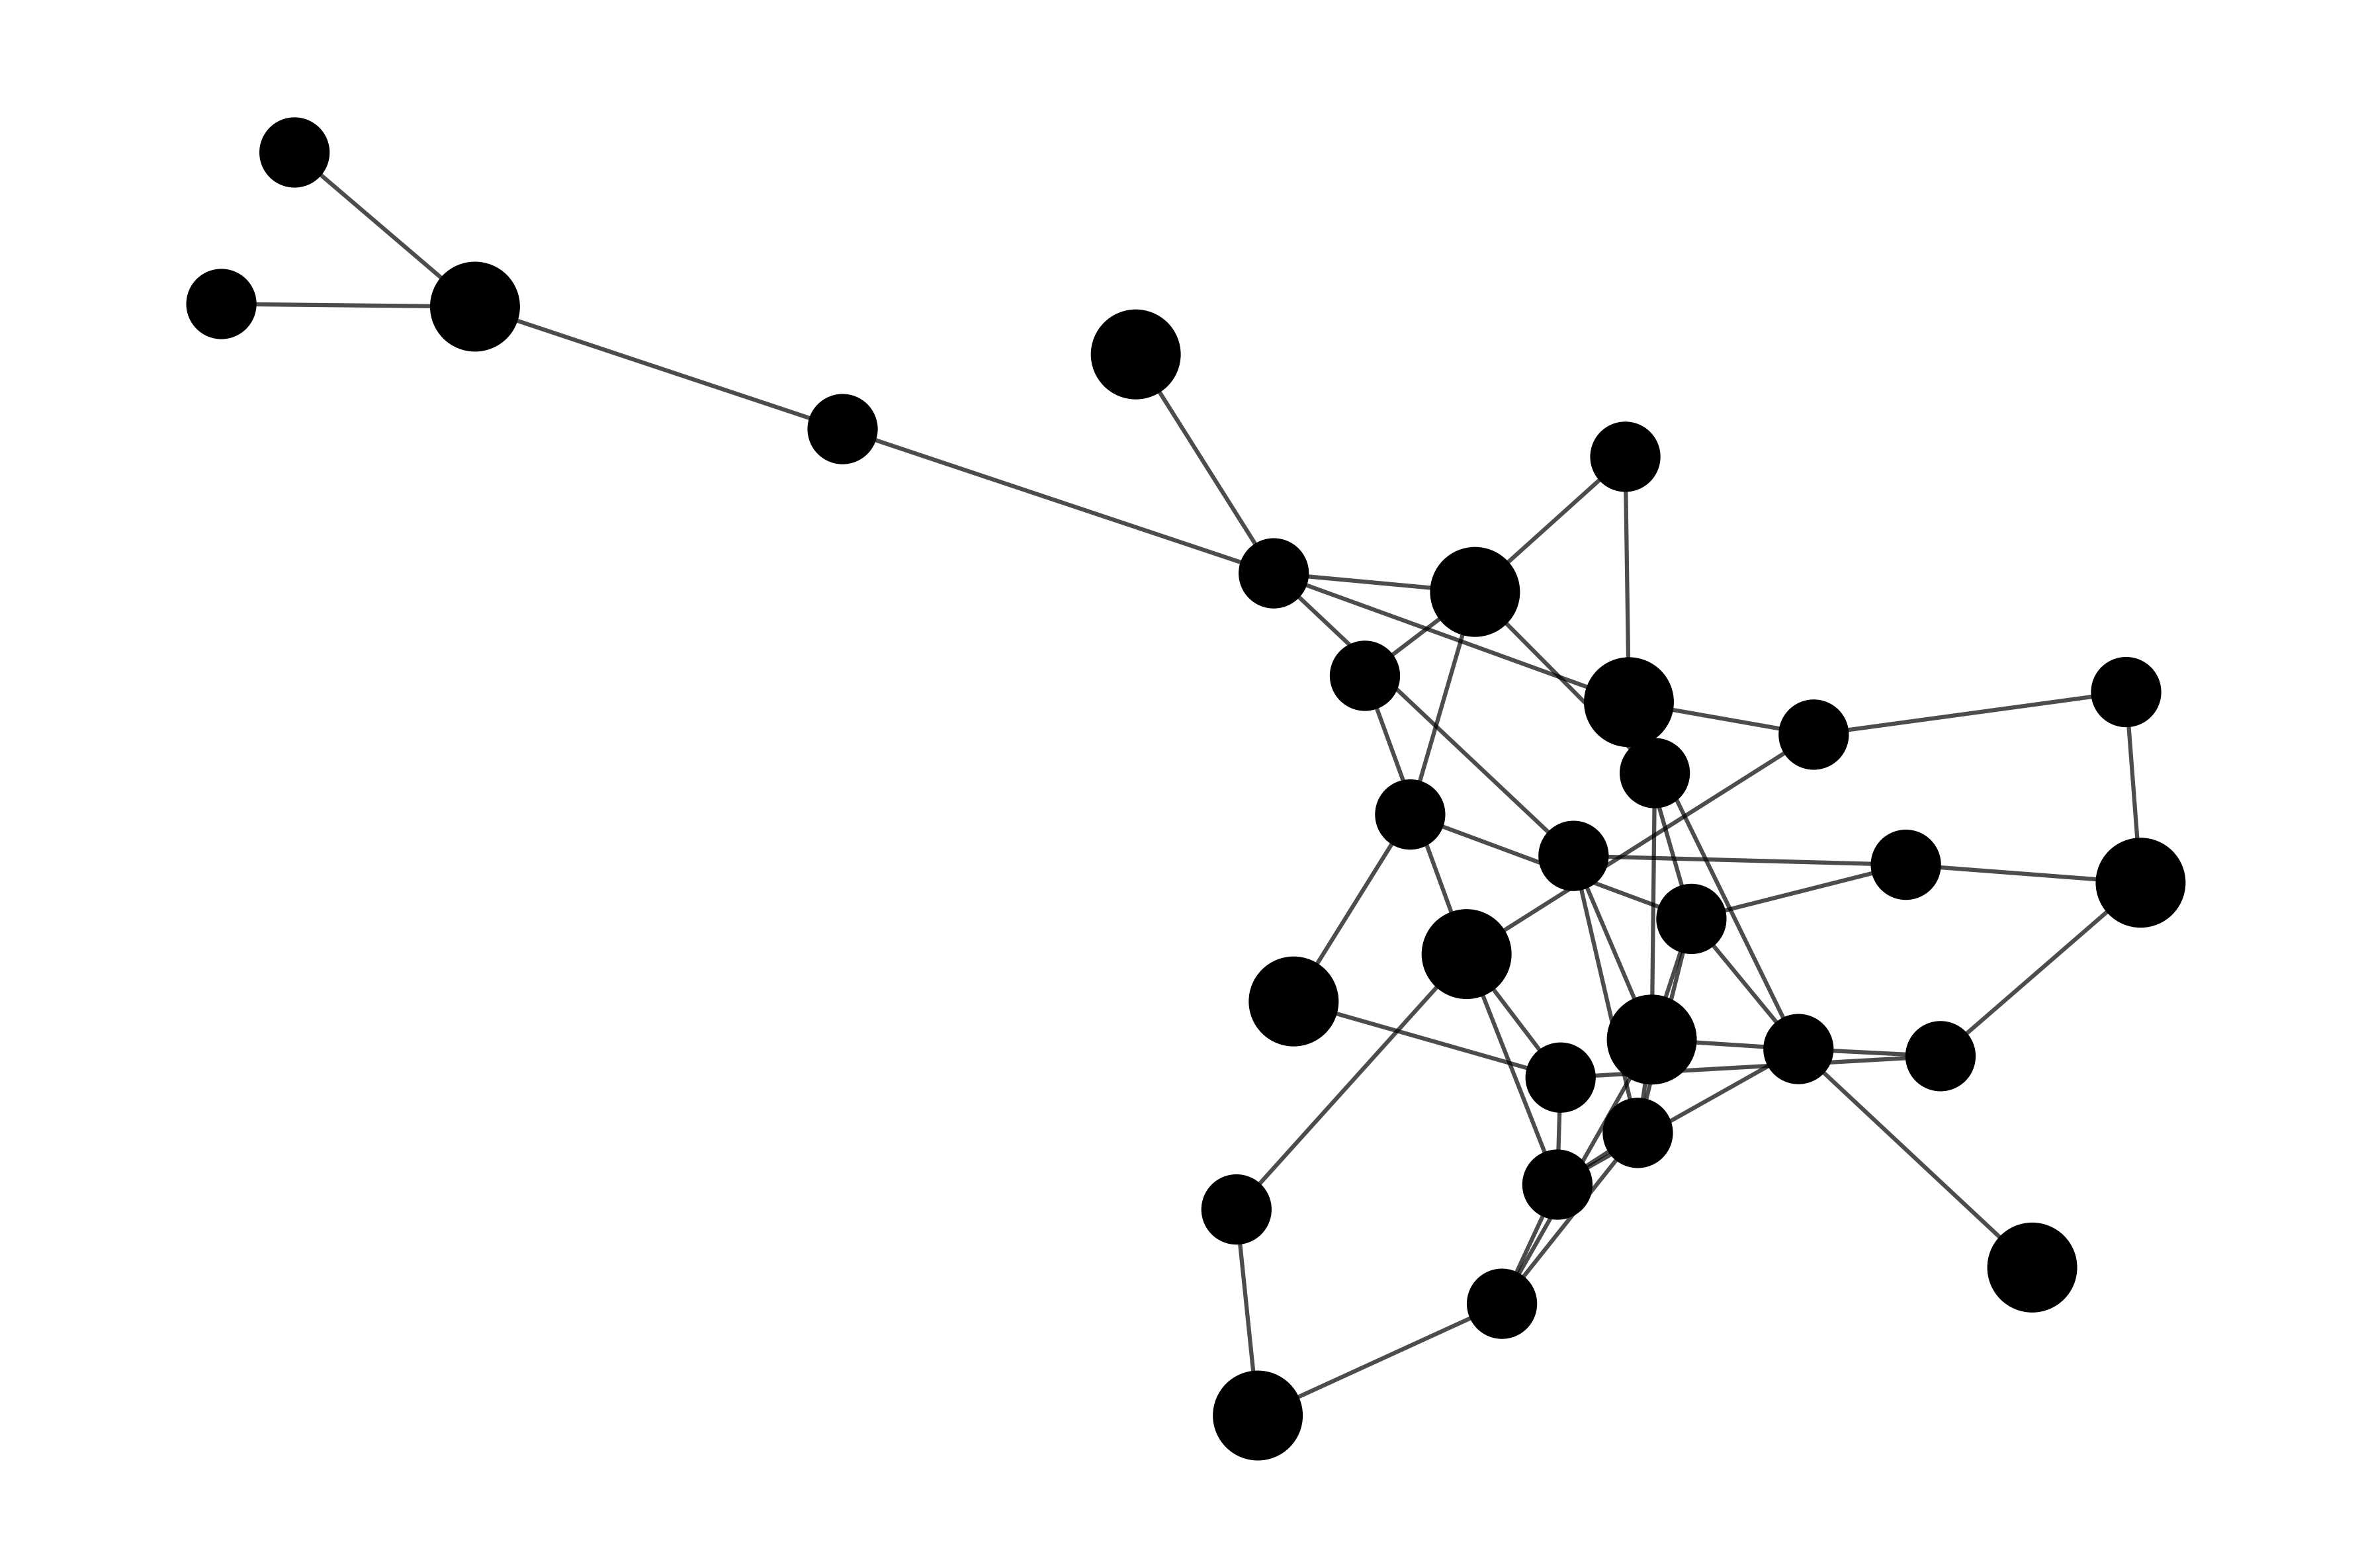
\includegraphics[width=0.6\textwidth]{assets/test_data/random.png}
    \caption{Przykładowa realizacja grafu Erdős--Rényi}
    \label{fig:ER}
\end{figure}

Model ER stanowi istotny punkt odniesienia jako najprostszy model sieci pozbawiony struktury społecznościowej. Motywacją uwzględnienia go w testach jest możliwość porównania działania algorytmów na zupełnie przypadkowych sieciach z ich działaniem na bardziej uporządkowanych grafach takich jak grafy skalowane, małego świata oraz rzeczywiste. Choć prawdziwe sieci społecznościowe odbiegają od założeń pełnej losowości, mają zwykle wyższy poziom klasteryzacji węzłów i nierównomierny rozkład stopni wierzchołków, to jednak model $G(n, p)$ stanowi istotną podstawę porównawczą.

Z punktu widzenia właściwości, grafy ER cechują się stosunkowo niskim średnim współczynnikiem klasteryzacji.
Współczynnik klasteryzacji mierzy, w jakim stopniu sąsiedzi danego wierzchołka są ze sobą połączeni. 
Dokładniej, oblicza się go jako stosunek liczby krawędzi faktycznie istniejących między sąsiadami wierzchołka do liczby wszystkich możliwych krawędzi między tymi sąsiadami. 
Średni współczynnik klasteryzacji dla całego grafu definiuje się jako średnią arytmetyczną wartości współczynników klasteryzacji po wszystkich wierzchołkach.
Oczekiwana wartość współczynnika klasteryzacji jest równa $p$ dla wystarczająco dużego $n$, a dla dostatecznie dużego $p$ istnieje możliwość powstania jednej gigantycznej składowej spójności.
Istnieje znana granica perkolacji, gdy $p>\frac{\ln n}{n}$, graf ER jest z dużym prawdopodobieństwem spójny - poniżej tego progu sieć rozpada się na wiele składowych \cite{ErdosRenyi1960}. Gęstość grafu, rozumiana jako odsetek istniejących krawędzi w stosunku do wszystkich możliwych, wynosi w tym modelu w przybliżeniu $p$. Przykładowo, dla $p=0.1$ graf będzie miał ok. 10\% maksymalnej liczby krawędzi. Rozkład stopni w modelu ER ma charakter dwumianowy, przy czym zbiega do rozkładu Poissona przy $n\to\infty$. Oznacza to, że w grafach tych nie występują węzły o niezwykle wysokich stopniach (tzw. huby), które są charakterystyczne dla wielu rzeczywistych sieci społecznościowych. W konsekwencji model ER nie oddaje wielu kluczowych właściwości takich sieci - stanowi jednak użyteczny model kontrolny, pozbawiony zjawisk typu mały świat czy skalowość, dzięki czemu można wyraźnie uwypuklić wpływ tych cech w innych modelach.


\subsection{Model Barabási--Albert - sieci bezskalowe}
Drugim wykorzystanym generatorem jest model Barabási--Albert (BA), wprowadzony przez Barabási'ego i Alberta w 1999 roku \cite{barabasi1999emergence}. Model BA pozwala generować grafy o strukturze bezskalowej, których rozkład stopni wierzchołków ma rozkład wykładniczy. Tego typu sieci charakteryzują się istnieniem niewielkiej liczby wierzchołków o bardzo wysokim stopniu (tzw. hubów) oraz wielu wierzchołków o małym stopniu - jest to cecha obserwowana w wielu rzeczywistych sieciach, w tym społecznościowych. Dla ilustracji, na rys.~\ref{fig:BA} przedstawiono przykładową realizację grafu BA, w której wyraźnie widoczne są huby. W przypadku sieci społecznościowych odnosi się to do tego, że niektórzy użytkownicy mogą mieć tysiące znajomych/obserwujących, podczas gdy większość ma ich kilkadziesiąt lub mniej.

\begin{figure}[h]
    \centering
    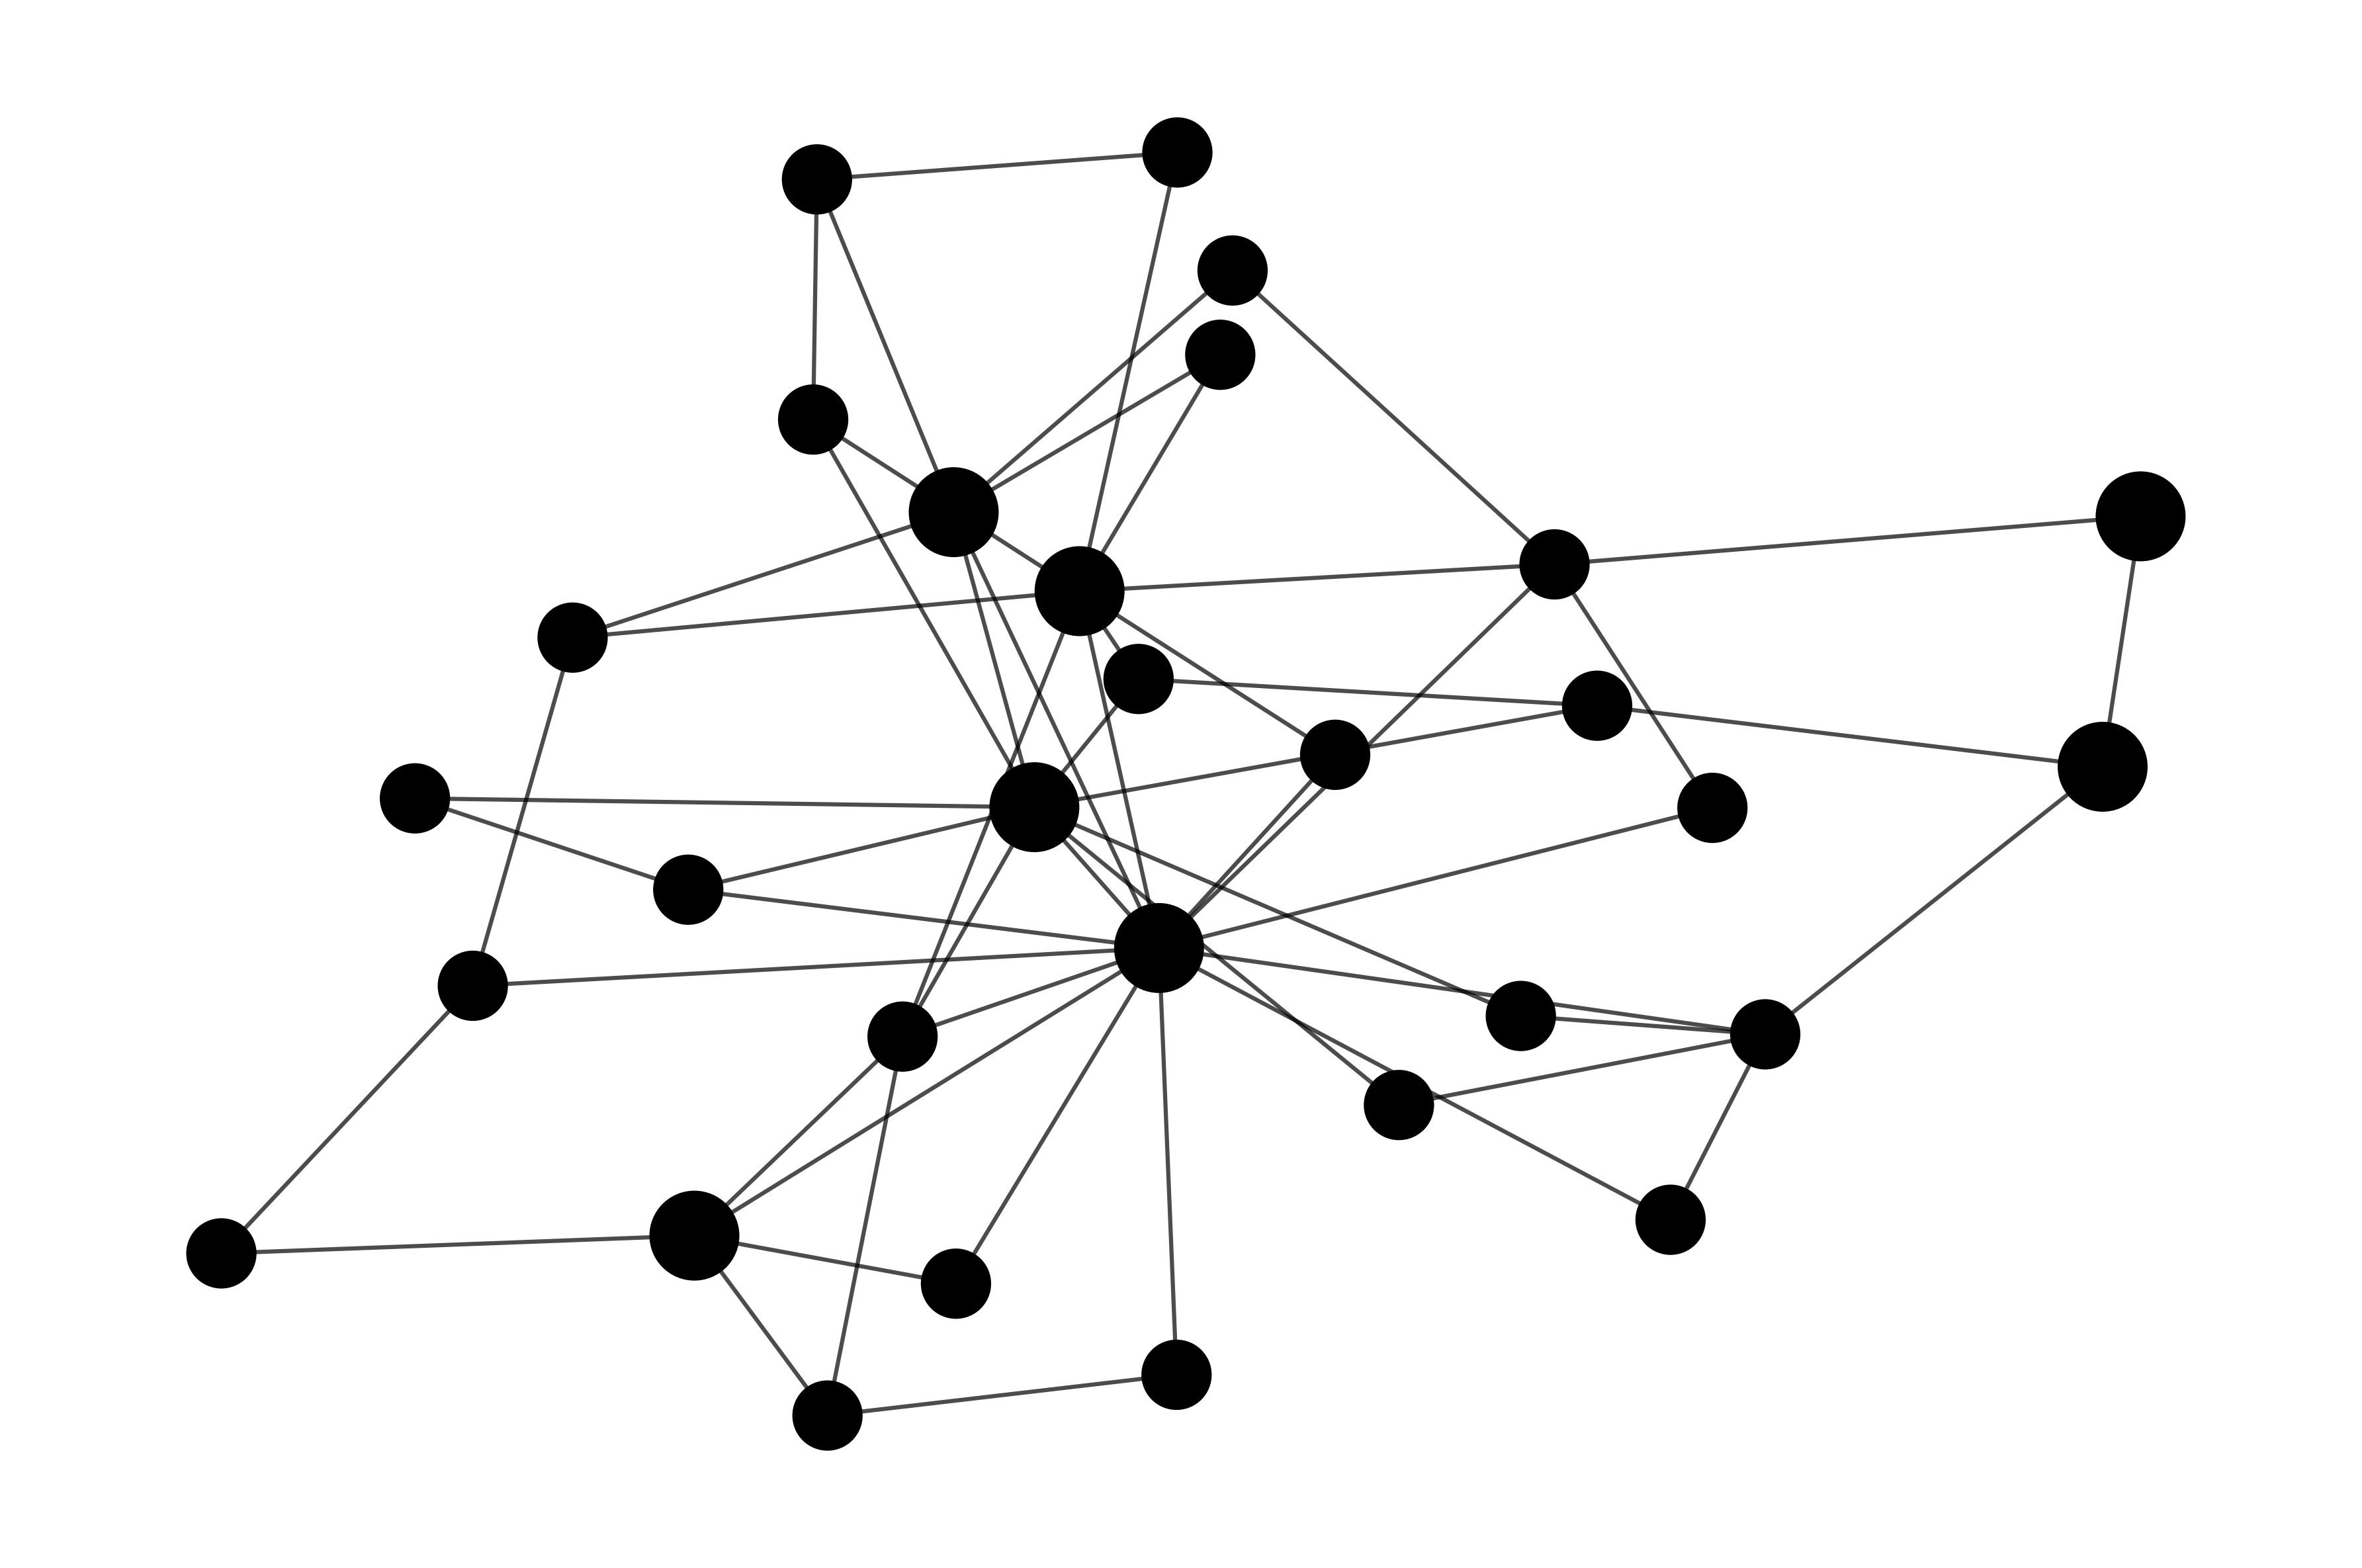
\includegraphics[width=0.6\textwidth]{assets/test_data/scalefree.png}
    \caption{Przykładowa realizacja grafu Barabási--Albert z widocznymi hubami}
    \label{fig:BA}
\end{figure}

Parametrem wejściowym modelu Barabási--Albert jest przede wszystkim $n$ - docelowa liczba węzłów w grafie - oraz $m$ - liczba krawędzi, jakie dodaje każdy nowy węzeł. Procedura generowania rozpoczyna się od małego grafu startowego (np. klika złożona z $m$ wierzchołków, aby zapewnić początkową spójność). Następnie dodaje się kolejno nowe wierzchołki; każdy nowy węzeł łączy się z $m$ już istniejącymi wierzchołkami, przy czym prawdopodobieństwo połączenia z danym istniejącym węzłem jest proporcjonalne do jego bieżącego stopnia (tzw. reguła preferencyjnego łączenia, ang. preferential attachment). Mechanizm preferencyjnego przyłączania zwiększa prawdopodobieństwo dalszego wzrostu stopnia wierzchołków o wysokiej liczbie połączeń, czyli wierzchołki, które zyskały wiele połączeń na wcześniejszych etapach, mają większą szansę zdobyć kolejne połączenia, co prowadzi do wykładniczego rozkładu stopni wierzchołków.

Motywacją użycia modelu BA było odzwierciedlenie w danych testowych właściwości często spotykanej w sieciach społecznościowych i sieciach informacji - silnego zróżnicowania w stopniach węzłów. Dzięki grafom BA można przetestować algorytmy pod kątem radzenia sobie z obecnością hubów oraz z rozkładem stopni o ciężkim ogonie (ang. heavy-tailed distribution). Pojęcie ciężkiego ogona oznacza, że prawdopodobieństwo wystąpienia wierzchołków o bardzo dużym stopniu maleje stosunkowo wolno - w efekcie w sieci, obok wielu węzłów o niskim stopniu, pojawia się również pewna liczba hubów o ekstremalnie wysokim stopniu. Zjawisko to odróżnia sieci bezskalowe od np. grafów ER, w których prawdopodobieństwo pojawienia się węzłów o bardzo dużej liczbie sąsiadów jest znikome.

Grafy generowane modelem BA mają z reguły jedną składową spójności. Przy założeniu, że graf początkowy jest spójny i $m \ge 1$, każdy nowy wierzchołek dołącza do istniejącej struktury, więc sieć pozostaje spójna, a średni stopień w takim grafie wynosi około $2m$. Stąd gęstość grafu BA maleje wraz ze wzrostem $n$. Dla dużych grafów jest ona rzędu $\frac{2m}{n}$, co oznacza, że grafy te są rzadkie. W przeciwieństwie do modelu ER, współczynnik klasteryzacji grafów BA nie jest determinowany przez pojedynczy parametr w oczywisty sposób - klasyczny model BA generuje sieci o stosunkowo niskim średnim współczynnikiem klasteryzacji (niższym niż obserwowany w rzeczywistych sieciach społecznościowych), ponieważ nowe połączenia tworzone są głównie z hubami, co sprzyja tworzeniu gwiazd zamiast trójkątów. Istnieją modyfikacje modelu BA dodające mechanizmy triadycznego dosłączania, które zwiększają współczynnik klasteryzacji - jednak w czystej postaci model BA zazwyczaj skutkuje średnim współczynnikiem klasteryzacji malejącym wraz z rozmiarem grafu. Niemniej jednak, nawet przy relatywnie niskim współczynniku klasteryzacji, grafy BA zachowują własność małych średnich odległości. Powyższe cechy sprawiają, że grafy BA stanowią przydatny model testowy - oddają one istnienie hubów i krótkich odległości jak w wielu sieciach społecznościowych, choć nie odwzorowują silnego grupowania lokalnego.

\subsection{Model Watts--Strogatz - graf małego świata}
Trzecim fundamentalnym modelem wykorzystanym w pracy jest model Watts--Strogatz (WS), opisany przez Wattsa i Strogatza w 1998 roku~\cite{Watts1998}. Umożliwia on generowanie grafów małego świata (small-world networks), które łączą w sobie dwie istotne cechy: wysoki współczynnik klasteryzacji (podobny do obserwowanego w sieciach regularnych) oraz niską średnią odległość (podobnie jak w grafach losowych). Model ten odzwierciedla fakt, że w sieciach społecznościowych często występują silnie zżyte grupy znajomych, a jednocześnie dowolne dwie osoby są połączone relatywnie krótką ścieżką znajomości.

Generacja grafu WS wymaga dostarczenia mu trzech parametrów: liczby wierzchołków, stopnia każdego wierzchołka w początkowej regularnej strukturze oraz prawdopodobieństwa istnienia krawędzi. Procedura rozpoczyna się od utworzenia grafu regularnego, gdzie każdy wierzchołek jest połączony z $k$ najbliższymi sąsiadami w cyklu (tj. tworzymy cykl z $n$ węzłów, a następnie każdy węzeł łączymy z $\frac{k}{2}$ następnymi i $\frac{k}{2}$ poprzednimi na cyklu, zakładając dla uproszczenia, że $k$ jest parzyste). Tak powstała sieć charakteryzuje się wysokim współczynnikiem klasteryzacji - węzły sąsiadujące na cyklu tworzą małe kliki.
Jednocześnie początkowa średnia odległość jest stosunkowo duża, bo graf tuż przed modyfikacją krawędzi ma strukturę cyklu, więc dystans między węzłami oddalonymi na cyklu jest znaczny. Na rys.~\ref{fig:WS} zilustrowano przykładową realizację grafu Watts--Strogatz, w której widoczne są opisane wyżej właściwości.

\begin{figure}[h]
    \centering
    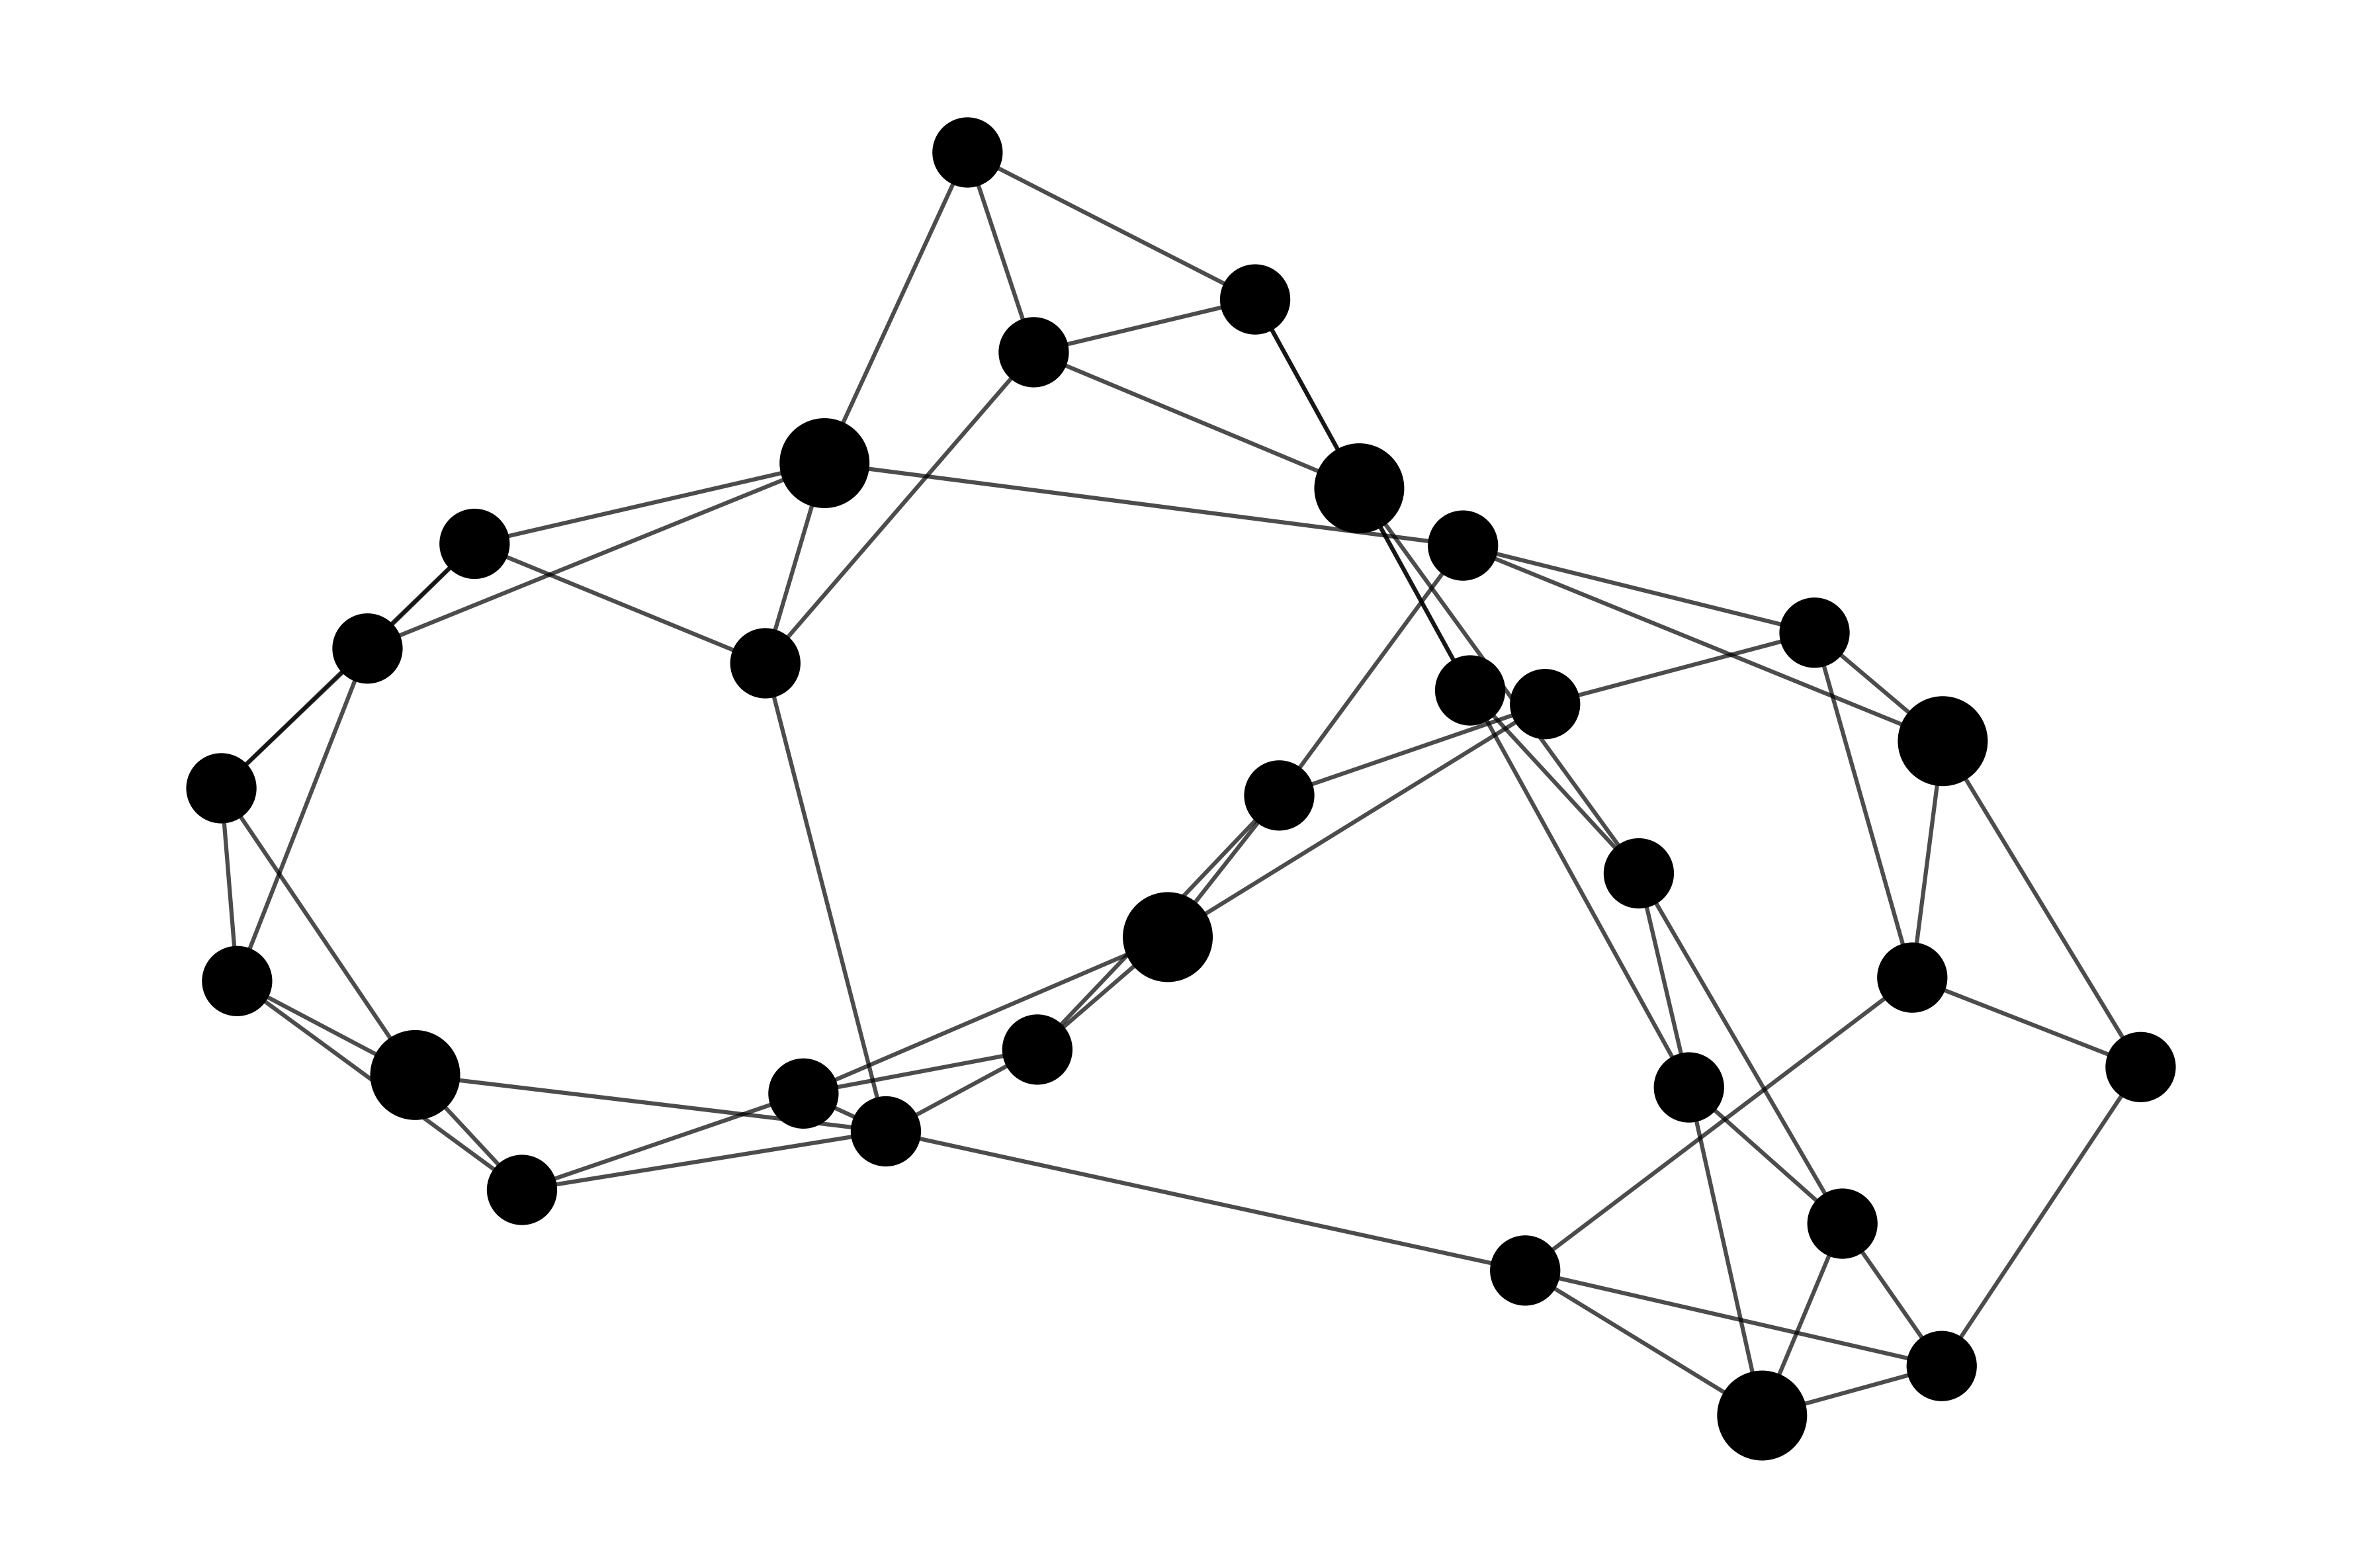
\includegraphics[width=0.65\textwidth]{assets/test_data/smallworld.png}
    \caption{Przykładowa realizacja grafu Watts--Strogatz, w której widoczne są lokalne kliki oraz losowe połączenia długodystansowe skracające średnie odległości}
    \label{fig:WS}
\end{figure}

Następnie, w modelu WS wprowadza się losowe przepięcia. Dla każdej krawędzi łączącej węzeł z jednym z $\frac{k}{2}$ najbliższych sąsiadów w cyklu. Dokonuje się, z prawdopodobieństwem $p$, przepięcia jednego końca tej krawędzi do losowo wybranego innego wierzchołka. Przepięcie polega na usunięciu oryginalnej krawędzi i dodaniu nowej krawędzi łączącej dany węzeł z innym losowym węzłem. W wyniku tych losowych przepięć, przy zachowaniu większości lokalnych połączeń cyklu, otrzymujemy graf, który dla małych $p$ wciąż charakteryzuje się wysokim współczynnikiem klasteryzacji, ale jednocześnie kilka losowych połączeń długodystansowych znacząco skraca średnie odległości w sieci. 
Dla umiarkowanych wartości $p$ (np. $p \approx 0.01$ czy $0.1$) sieć uzyskuje bardzo małą średnią odległość - zbliżoną do grafów losowych - podczas gdy współczynnik klasteryzacji pozostaje o rząd wielkości wyższy niż w grafie Erdős--Rényi o porównywalnej gęstości.

W kontekście modelowania sieci społecznościowych, generator dla modelu WS dodano w celu odzwierciedlenia właściwości, których brakuje modelowi BA - mianowicie wysokiego lokalnego współczynnika klasteryzacji. Sieci społecznościowe cechują się tym, że znajomi często znają się nawzajem, tworząc kliki znajomych. Model WS pozwala symulować taką sytuację i sprawdzić, jak algorytmy radzą sobie np. z wykrywaniem społeczności czy zjawisk rozprzestrzeniania się informacji w warunkach silnego grupowania. Parametr $k$ decyduje o początkowej gęstości połączeń lokalnych - większe $k$ to więcej krawędzi lokalnych (każdy węzeł ma początkowo $k$ sąsiadów), a zatem wyjściowo wyższy współczynnik klasteryzacji i gęstość. Parametr $p$ kontroluje losowość grafu. 
Dla $p=0$ otrzymujemy graf regularny, natomiast dla $p=1$ graf staje się w dużej mierze losowy. 
W praktycznych zastosowaniach szczególnie interesujący jest zakres wartości $p$ pomiędzy 0 a 1, w którym sieć łączy wysoki współczynnik klasteryzacji z niewielką średnią odległością między wierzchołkami.


Grafy WS generowane do testów miały parametry dobrane w taki sposób, aby możliwie dobrze odwzorowywać cechy typowe dla niedużych sieci społecznościowych. Uzyskiwane w ten sposób sieci charakteryzowały się relatywnie niską gęstością, ale jednocześnie wysokim współczynnikiem klasteryzacji, znacznie przewyższającym wartości obserwowane w losowych grafach ER o podobnej gęstości. Dzięki temu w grafach WS obecne są realistyczne zgrupowania lokalne, odpowiadające typowym kręgom znajomych w sieciach społecznościowych. Co istotne, sieci te z reguły pozostają spójne - niemal wszystkie wierzchołki należą do jednej dużej składowej spójności, a ewentualne izolowane węzły pojawiają się jedynie sporadycznie przy skrajnych ustawieniach parametrów. Taka struktura sprawia, że model WS stanowi dobre środowisko testowe.

\section{Grafy rzeczywiste}
Drugim zestawem danych testowych są rzeczywiste grafy pochodzące z sieci społecznościowej Facebook,
a dokładniej zbiór Facebook Ego Network udostępniony w ramach Stanford Network Analysis Project (SNAP)~\cite{snapnets}.
Dane te zostały zebrane w 2012 roku przez J. McAuley i J. Leskovca z Uniwersytetu Stanforda w ramach badań nad automatycznym wykrywaniem kręgów społecznościowych~\cite{McAuley2012}. Zbiór zawiera dziesięć tzw. ego-sieci, czyli sieci ego-centrycznych poszczególnych użytkowników Facebooka, pozyskane za zgodą uczestników przy użyciu dedykowanej aplikacji badawczej działającej w ramach platformy Facebook. Ego-sieć to sieć społecznościowa zbudowana z perspektywy pojedynczego użytkownika zwanego ego - węzłami są ego oraz wszystkie jego bezpośrednie znajome osoby, zaś krawędzie reprezentują relacje znajomości pomiędzy tymi znajomymi. W udostępnionych danych każda z dziesięciu sieci odpowiada innemu użytkownikowi i zawiera wyłącznie jego znajomych oraz powiązania między nimi. Węzeł ego nie jest jawnie ujęty jako wierzchołek w grafie i można go traktować jako ukrytą centralną jednostkę łączącą wszystkich znajomych. Innymi słowy, graf zapisany w pliku \verb|X.edges| dotyczy tylko znajomych użytkownika $X$ i relacji między nimi - sam $X$ nie pojawia się w pliku jako węzeł.

\subsection{Struktura danych}

Każda ego-sieć udostępnione przez SNAP zapisana jest w osobnych plikach tekstowych, których nazwa odpowiada identyfikatorowi \textit{ego} (np. \verb|0.edges|, \verb|0.circles|, \verb|0.feat|, \verb|0.egofeat| dla \textit{ego} o ID=0). Struktura danych jest następująca:

\textbf{Plik .edges} - lista krawędzi w grafie znajomych danego ego. Każdy wiersz zawiera dwie liczby - identyfikatory dwóch różnych znajomych ego, między którymi istnieje relacja koleżeńska. Krawędzie te są nieskierowane. Ważną cechą jest to, że plik \verb|.edges| nie zawiera połączeń od ego do jego znajomych - wierzchołek ego w ogóle nie występuje w tym pliku. Oznacza to, że rzeczywista sieć ego (gdyby uwzględnić w niej węzeł ego) miałaby dodatkowo krawędź łączącą ego z każdym z pojawiających się znajomych, jednak tych połączeń tutaj nie zapisano (są one domyślne - zakładamy, że ego jest połączone ze wszystkimi swoimi znajomymi). Pominięcie węzła ego jest zabiegiem celowym, pozwalającym skupić się na relacjach wewnątrz kręgów znajomych. Konsekwencją tego jest często podział grafu znajomych na kilka składowych - jeśli ego ma różne grupy znajomych wzajemnie się nieznających, to w pliku \verb|.edges| każda taka grupa stanowi osobną składową spójności. Przykładowo, w ego-sieci \verb|0.edges| znajomi tworzą 5 odrębnych składowych spójności. Oznacza to, że użytkownik o ID 0 miał około pięć niezależnych grup znajomych niepowiązanych ze sobą - dopiero poprzez jego osobę stawały się one pośrednio połączone.

\textbf{Plik .circles} - zestaw kręgów znajomych zdefiniowanych przez użytkownika. Każdy wiersz pliku reprezentuje jeden krąg towarzyski. Wiersz rozpoczyna się od nazwy kręgu - jednak w udostępnionych danych nazwy te zostały zanonimizowane lub pominięte, więc w praktyce każdy wiersz zaczyna się od identyfikatora kręgu albo pustej nazwy, po czym następuje lista ID użytkowników należących do tego kręgu. Kręgi mogą częściowo się pokrywać i nie muszą stanowić rozłącznych społeczności w sensie grafu - są to raczej dodatkowe metadane od ego, opisujące jak kategoryzuje on swoich znajomych. Informacje te mogą być cenne pomocniczo, np. w oryginalnej pracy McAuley'ego i Leskovca posłużyły do oceny algorytmów automatycznie wykrywających społeczności~\cite{McAuley2012}.

\textbf{Plik .feat} - macierz cech atrybutów przypisanych do znajomych ego. Każdy wiersz odpowiada jednemu znajomemu i zawiera wektor wartości cech tej osoby. Cechy te mogą obejmować informacje z profilu Facebooka (np. miejsce pracy, szkoła, zainteresowania itp.). W udostępnionym zbiorze wartości atrybutów zostały zanonimizowane - nie znamy dokładnego znaczenia poszczególnych cech, jedynie ich binarne wartości (1 - użytkownik posiada daną cechę, 0 - nie posiada). Istnieje także plik \verb|.featnames| zawierający oryginalne nazwy cech, ale w przypadku Facebooka nazwy te również zostały zanonimizowane (np. zamiast "szkoła: Uniwersytet Stanford" pojawia się anonimowa cecha 57). W niniejszej pracy dane atrybutów nie były wykorzystywane przez algorytmy i skupiono się tylko na strukturze grafów.

\textbf{Plik .egofeat} - wektor cech centralnego użytkownika, w tym samym formacie co pojedynczy wiersz pliku \verb|.feat|, odnoszący się jednak do ego. Pozwala to porównać cechy ego z cechami jego znajomych. W kontekście naszych badań plik ten również nie był bezpośrednio wykorzystywany, poza podstawową walidacją danych.

W eksperymentach wykorzystano wszystkie dziesięć ego-sieci dostępnych w zbiorze SNAP. Liczba węzłów (po pominięciu centralnego ego) wynosiła odpowiednio 53, 62, 151, 169, 225, 334, 535, 748, 787 oraz 1035. Tak szeroki zestaw umożliwił ocenę algorytmów zarówno na niewielkich, jak i ponadtysięcznych grafach, w których różnice w gęstości i strukturze społeczności są wyraźnie widoczne.

\subsection{Szczegółowy opis danych ze zbioru SNAP}
W badanym zbiorze występują zarówno niewielkie sieci liczące poniżej setki węzłów (np. ID 3980: 53 wierzchołki, 252 krawędzie), jak i bardzo duże instancje przekraczające tysiąc węzłów (ID 0: 1035 wierzchołków, ponad 26\,000 krawędzi). Ogólnie rzecz biorąc, większa liczba znajomych oznacza większe zróżnicowanie strukturalne: część ego-sieci składa się z kilku gęstych społeczności, podczas gdy inne są rozproszone i tworzą liczne składowe. Sumarycznie wszystkie dziesięć ego-sieci obejmuje 4039 unikalnych wierzchołków oraz 88\,234 krawędzie \cite{McAuley2012}, co dobrze oddaje skalę i złożoność sieci osobistych kontaktów.

Jak wspomniano, z powodu braku węzła ego w grafie znajomych większość ego-sieci dzieli się na więcej niż jedną składową spójności. W praktyce zazwyczaj istnieje jedna dominująca składowa, zawierająca największą grupę wzajemnie powiązanych znajomych, oraz kilka mniejszych składowych (np. dwu- lub kilkuosobowych grup) odpowiadających odizolowanym kręgom towarzyskim. Dla przykładu, sieć \verb|107.edges| okazała się całkowicie spójna - wszyscy znajomi użytkownika 107 tworzyli jeden graf spójny. Natomiast sieć \verb|0.edges| miała 5 składowych - co już sygnalizowano wcześniej. Wśród naszych analizowanych sieci: sieć \verb|686.edges| jest spójna, sieć \verb|414.edges| dzieli się na 2 składowe, sieć \verb|698.edges| na 3, a sieć \verb|3980.edges| na 4 składowe. Zwykle największa składowa obejmuje zdecydowaną większość wierzchołków. Taka struktura wskazuje na obecność jednego głównego kręgu znajomych, uzupełnionego kilkoma mniejszymi grupami znajomości niepowiązanych z resztą.

Ego-sieci Facebooka cechują się na ogół wysokim współczynnikiem klasteryzacji, co zgodne jest z intuicją - znajomi konkretnej osoby często znają się nawzajem. W literaturze podaje się, że globalny współczynnik klasteryzacji dla całego grafu Facebooka jest stosunkowo niski~\cite{Ugander2011}. W obrębie pojedynczej ego-sieci, gdzie wszyscy rozważani ludzie są znajomymi jednego ego, współczynnik klasteryzacji jest znacznie wyższy. Dla połączonej sieci 10 ego (4039 węzłów) średni współczynnik klasteryzacji wynosił aż 0.6055, co oznacza, że dwaj losowo wybrani znajomi danego ego mieli ponad 60\% szans, by również być znajomymi między sobą. W naszych mniejszych sieciach wartości te różnią się w zależności od sieci, ale zwykle mieszczą się w przedziale 0.5-0.6 dla największej składowej (mniejsze składowe, np. dwuosobowe, mają współczynnik klasteryzacji równy 0 lub nieokreślony). Wysoki średni współczynnik klasteryzacji potwierdza istnienie silnych lokalnych powiązań - w grafie występuje wiele trójkątów (grup znajomych, z których każdy zna pozostałych). Przykładowo, jeśli ego posiada grupę bliskich przyjaciół ze szkoły, to prawdopodobne jest, że większość z nich zna się nawzajem, tworząc pełne podgrafy (kliki) o dużym współczynniku klasteryzacji.

W ego-sieciach Facebooka obserwuje się niskie wartości gęstości, co odzwierciedla ogólną rzadkość połączeń charakterystyczną dla sieci społecznościowych. Typowe wartości w badanym zbiorze mieszczą się od kilku do kilkunastu procent. Największe sieci (powyżej 700 węzłów) osiągają gęstości około 5\%, natomiast mniejsze instancje (53 i 62 węzły) przekraczają 15\% dzięki bardziej lokalnym połączeniom. W porównaniu do grafów losowych o podobnej skali ego-sieci mają wyższy współczynnik klasteryzacji (krawędzie nie są rozłożone przypadkowo, lecz skoncentrowane wewnątrz podzbiorów wierzchołków). Ta rzadka natura sieci społecznościowych jest istotna z punktu widzenia testowanych algorytmów, gdyż wiele z nich ma złożoności silnie zależne od liczby krawędzi (np. operacje przeszukiwania grafu lub znajdowania struktur klikowych mogą być szybsze w grafach rzadszych).

\chapter{Metody algorytmiczne}\label{chap:algorithms}

W tym rozdziale przedstawiono wszystkie algorytmy zastosowane w pracy. Każdy algorytm opisano wraz z jego główną ideą, parametrami oraz analizą złożoności obliczeniowej.


Algorytmy zastosowane w pracy można podzielić na trzy grupy:
\begin{enumerate}
  \item \textbf{Metody dokładne} -- gwarantują znalezienie optymalnego rozwiązania: algorytm naiwny i programowanie całkowitoliczbowe (ILP).
  \item \textbf{Heurystyki konstrukcyjne} -- szybkie metody budujące rozwiązanie krok po kroku: algorytm zachłanny, zbiór dominujący, algorytm losowy.
  \item \textbf{Metaheurystyki} -- zaawansowane metody przeszukujące przestrzeń rozwiązań: algorytm genetyczny, przeszukiwanie tabu, algorytm mrówkowy, symulowane wyżarzanie.
\end{enumerate}

\section{Metody dokładne}

\subsection{Algorytm naiwny}\label{subsec:naive}
Algorytm naiwny jest metodą dokładną. Przegląda wszystkie podziały zbioru wierzchołków na dopuszczalne grupy oraz wszystkie przypisania licencji. Wybierane jest rozwiązanie o najniższym koszcie. Liczba rozważanych konfiguracji rośnie wykładniczo, dlatego metoda ma znaczenie praktyczne tylko dla bardzo małych instancji.

Na rysunku \ref{fig:all_types_time} przedstawiono czasy obliczeń w funkcji liczby wierzchołków dla grafów losowych, małoświatowych i bezskalowych. Do 12 wierzchołków czas wykonania pozostaje akceptowalny dla celów eksperymentalnych. Z uwagi na wykładniczy wzrost czasu działania algorytmu metoda ta staje się niepraktyczna dla większych instancji, zwłaszcza w kontekście dostępności bardziej efektywnych algorytmów, takich jak programowanie całkowitoliczbowe (ILP).

\begin{figure}[H]
  \centering
  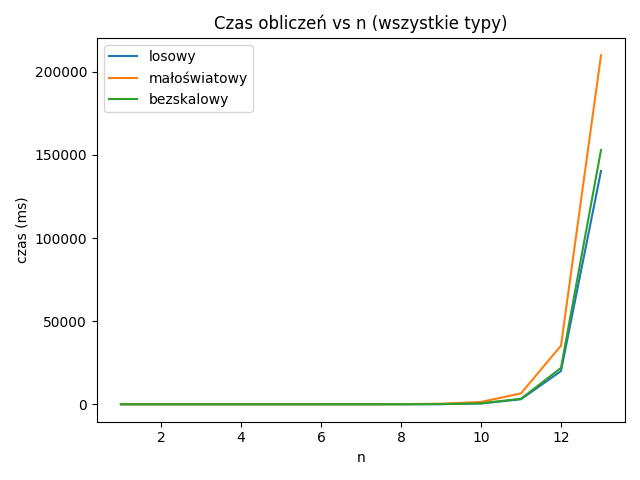
\includegraphics[width=0.66\textwidth]{assets/all_types_plot.png}
  \caption{Czas obliczeń algorytmu naiwnego w funkcji liczby wierzchołków $n$ dla trzech typów grafów}
  \label{fig:all_types_time}
\end{figure}

\paragraph{Idea metody}
\begin{enumerate}
  \item Wygenerować wszystkie partycje zbioru \(V\) na niepuste bloki (każdy blok odpowiada kandydatowi na grupę licencyjną).
  \item Dla każdego bloku w danej partycji wypisać wszystkie dopuszczalne pary (właściciel, licencja), czyli takie, które spełniają ograniczenia pojemności oraz sąsiedztwa.
  \item Łączyć wybory z poszczególnych bloków w pełne przypisania i odrzucać te, które nie pokrywają wierzchołków lub łamią ograniczenia.
  \item Obliczyć koszt na podstawie funkcji kosztu $\cost(f)$ (\ref{eq:cost_function}) i zapamiętać najlepsze rozwiązanie.
\end{enumerate}

\begin{algorithm}[H]
  \caption{Algorytm naiwny: pełny przegląd rozwiązań}
  \label{alg:naive}
  \begin{algorithmic}[1]
    \Require graf \(G=(V,E)\), zbiory licencji \( L\)
    \If{\(|V|>12\)} \State \Return przerwanie z powodu ograniczenia eksperymentalnego \EndIf
    \State \(best\_cost \gets \infty\), \(best \gets \emptyset\)
    \For{każda partycja \(P=\{P_1,\dots,P_k\}\) zbioru \(V\)}
    \For{każde przypisanie \(l\in L\) i właściciela w każdym \(P_i\)}
    \If{spełnione pojemności, sąsiedztwo i pełne pokrycie}
    \State policz koszt; zaktualizuj \(best\), jeśli lepszy
    \EndIf
    \EndFor
    \EndFor
    \State \Return \(best\)
  \end{algorithmic}
\end{algorithm}

\paragraph{Złożoność}
Algorytm generuje wszystkie partycje zbioru \(V\) na niepuste bloki, czyli wszystkie rozbicia odpowiadające potencjalnym zestawom grup licencyjnych. Takich partycji jest \(B_{|V|}\), gdzie \(B_m\) oznacza liczbę Bella dla \(m\) elementów \cite{stanley1997enumerative}. W implementacji nie ograniczamy z góry liczby bloków: niektóre typy licencji mogą pozostać nieużyte, dlatego dopuszczamy zarówno rozbicia na jedną grupę, jak i na \(|V|\) grup jednowierzchołkowych. Gdyby liczba bloków była stała i wynosiła \(k\), odpowiadałyby jej liczby Stirlinga drugiego rodzaju \({|V| \brace k}\); tutaj sumujemy je po wszystkich \(k\), stąd pojawiają się liczby Bella. Samo wygenerowanie partycji kosztuje więc $\Theta(B_{|V|})$.

Dla partycji o \(k\) blokach o rozmiarach \(s_1, s_2, \ldots, s_k\) rozpatrujemy każdą kombinację wyboru właściciela (co najwyżej \(s_i\) opcji na blok \(i\)) i dopuszczalnego typu licencji (co najwyżej \(T\) opcji, gdzie \(T=|L|\)). Prowadzi to do górnego oszacowania
\[
  \prod_{i=1}^{k} (s_i \cdot T) = T^k \cdot \prod_{i=1}^{k} s_i
\]
konfiguracji dla pojedynczej partycji. Całkowity koszt można oszacować przez \(O\bigl(B_{|V|} \cdot T^{|V|} \cdot 3^{|V|/3}\bigr)\), ponieważ \(\prod s_i \leq 3^{|V|/3}\). Wzrost jest superwykładniczy, gdzie asymptotycznie \(\log B_n = n\log n - n\log\log n - n + O(n/\log n)\). W praktyce ograniczenia licencyjne i warunek sąsiedztwa znacząco zmniejszają liczbę rozważanych konfiguracji, lecz nawet wtedy pełny przegląd jest użyteczny wyłącznie dla bardzo małych grafów (rzędu kilku do kilkunastu wierzchołków).

Liczby Bella można zapisać wzorami
\[
  B_n = \sum_{k=0}^{n} \left\{\!\!\begin{array}{c} n \\ k \end{array}\!\!\right\}\quad\text{oraz}\quad B_n = \frac{1}{e}\sum_{k=0}^{\infty}\frac{k^{\,n}}{k!},
\]
a zliczają one wszystkie rozbiory zbioru na dowolną liczbę niepustych bloków (bloki są nierozróżnialne). Dla porównania liczba wszystkich podzbiorów zbioru \(n\)-elementowego wynosi jedynie \(2^n\), więc nawet tak uproszczone oszacowanie rośnie wolniej niż pełna liczba partycji.

\subsection{Programowanie całkowitoliczbowe (ILP)}\label{subsec:ilp}

Formułujemy problem z rozdziału~\ref{sec:model-formal} jako minimalizację kosztu przy ograniczeniach liniowych z binarnymi zmiennymi. Model jest dokładny; solver zwraca rozwiązanie optymalne, jeśli zakończy działanie poprawnie.

\paragraph{Parametry i zmienne}
Korzystamy z rodziny licencji z~\eqref{eq:license_family},
\(\mathcal{L}=\{\ell_t=(c_t,m_t,k_t):t=1,\dots,T\}\).
Oznaczamy \(N[i]=N(i)\cup\{i\}\). Dla \(i\in V\), \(t\in\{1,\dots,T\}\) definiujemy:
\begin{itemize}
  \item \(a_{i,t}\in\{0,1\}\): \(a_{i,t}=1\) gdy węzeł \(i\) kupuje licencję typu \(t\) i aktywuje grupę,
  \item \(x_{i,j,t}\in\{0,1\}\) dla \(j\in N[i]\): \(x_{i,j,t}=1\) gdy \(j\) należy do grupy właściciela \(i\) typu \(t\).
\end{itemize}
Zmienna \(x_{i,j,t}\) odwzorowuje przypisanie odbiorcy do właściciela; zbiory ról są indukowane przez wartości \((a,x)\).

\paragraph{Model}
\begin{align}
  \min\quad & \sum_{i\in V}\sum_{t=1}^{T} c_t\, a_{i,t}                                                                        \\
  \text{pod warunkami:}\quad
            & \sum_{i\in N[j]}\sum_{t=1}^{T} x_{i,j,t} = 1
            &                                                                & \forall j\in V \label{con:cover}                \\
            & m_t\, a_{i,t} \le \sum_{j\in N[i]} x_{i,j,t} \le k_t\, a_{i,t}
            &                                                                & \forall i\in V,\ \forall t \label{con:capacity} \\
            & x_{i,i,t} = a_{i,t}
            &                                                                & \forall i\in V,\ \forall t \label{con:owner}    \\
            & \sum_{t=1}^{T} a_{i,t} \le 1
            &                                                                & \forall i\in V \label{con:one}
\end{align}

Znaczenie ograniczeń: \eqref{con:cover} pokrywa każdy węzeł dokładnie raz; \eqref{con:capacity} wymusza przedziały wielkości grup; \eqref{con:owner} zapewnia udział właściciela; \eqref{con:one} ogranicza do jednej licencji na węzeł (dowolnego typu). Ograniczenia pokrywają warunki wykonalności z rozdziału~\ref{sec:model-formal}.

\paragraph{Złożoność}
Liczba zmiennych: \(|V|T\) dla \(a_{i,t}\) oraz \(T\sum_i |N[i]|\) dla \(x_{i,j,t}\), łącznie \(O\!\bigl(T(|E|+|V|)\bigr)\).
Liczba ograniczeń: \(|V|\) dla \eqref{con:cover}, \(2|V|T\) dla \eqref{con:capacity}, \(|V|T\) dla \eqref{con:owner}, \(|V|\) dla \eqref{con:one}.
Model służy jako punkt odniesienia dla małych i średnich instancji.

\paragraph{Implementacja}
Implementacja w Python (PuLP + CBC) odzwierciedla powyższy model. Stosuje się eliminację niemożliwych par \((i,t)\), gdy \(m_t>|N[i]|\) lub \(k_t<1\), oraz dla \(k_t=1\) tworzy się wyłącznie zmienne \(x_{i,i,t}\).
Przy rekonstrukcji rozwiązania wartości binarne interpretowane są progowo \(>0{,}5\).
W razie statusu innego niż rozwiązanie całkowite zastosowano awaryjny wariant „same licencje indywidualne" (procedura poza modelem).

\section{Heurystyki konstrukcyjne}

\subsection{Algorytm zachłanny}\label{subsec:greedy}

Algorytm zachłanny to szybka heurystyka, która buduje rozwiązanie krok po kroku, w każdym kroku wybierając lokalnie najlepszą opcję. Algorytm nie gwarantuje znalezienia optymalnego rozwiązania, ale jest bardzo szybki i daje zazwyczaj w miarę dobre wyniki.

\paragraph{Idea metody}
Algorytm działa według następującej strategii:
\begin{enumerate}
  \item Sortuje wierzchołki nierosnąco według liczby sąsiadów (stopnia wierzchołka).
  \item Dla każdego wierzchołka sprawdza, czy może być właścicielem grupy.
  \item Wybiera typ licencji i rozmiar grupy tak, aby zminimalizować stosunek kosztu do rozmiaru grupy.
  \item Dodaje członków do grupy wybierając wierzchołki o największej liczbie sąsiadów.
  \item Powtarza proces dla wszystkich niepokrytych wierzchołków.
\end{enumerate}

Algorytm nie ma parametrów do dostrajania. Wszystkie decyzje są podejmowane deterministycznie na podstawie struktury grafu i kosztów licencji, choć w przypadku wierzchołków o tym samym stopniu kolejność wyboru może wpływać na wynik końcowy.

Sortowanie według stopnia wierzchołka (liczby sąsiadów) sprawdza się dobrze w praktyce, ponieważ wierzchołki o wysokim stopniu mogą tworzyć większe, bardziej efektywne grupy licencyjne.

\begin{algorithm}[H]
  \caption{Algorytm zachłanny}
  \label{alg:greedy}
  \begin{algorithmic}[1]
    \Require graf $G=(V,E)$, typy licencji $ L$
    \State posortuj wierzchołki nierosnąco według stopnia
    \State $niepokryte \gets V$
    \For{każdy wierzchołek $v$ w posortowanej kolejności}
    \If{$v$ już pokryty} \textbf{continue} \EndIf
    \State znajdź dostępnych sąsiadów $v$ wśród niepokrytych
    \For{każdy typ licencji $l_t \in L$}
    \State oblicz efektywność: $koszt_{l_t} / rozmiar\_grupy$
    \EndFor
    \State wybierz licencję i członków grupy o najlepszej efektywności
    \State utwórz grupę z $v$ jako właścicielem
    \State usuń członków grupy z $niepokryte$
    \EndFor
    \State \Return utworzone grupy
  \end{algorithmic}
\end{algorithm}


\paragraph{Złożoność i zastosowanie}
Algorytm ma złożoność czasową $O(|V|\,T + |E|\log |V|)$, gdzie $|V|$ to liczba wierzchołków, $|E|$ to liczba krawędzi, a $T$ to liczba typów licencji.
Algorytm zachłanny jest bardzo szybki i daje stabilne wyniki. Z tego powodu często używany był jako:
\begin{itemize}
  \item podstawowa metoda do porównywania z innymi algorytmami,
  \item źródło rozwiązania początkowego dla bardziej zaawansowanych metod,
  \item szybka metoda dla dużych grafów, gdzie inne algorytmy są zbyt wolne.
\end{itemize}
Wadą algorytmu jest to, że podejmując lokalnie najlepsze decyzje, może przegapić lepsze rozwiązania globalne.
\subsection{Heurystyka zbioru dominującego}\label{subsec:ds}

Heurystyka korzysta z konstrukcji \emph{minimalnych względem inkluzji} zbiorów dominujących. Zbiór dominujący jest minimalny, gdy usunięcie dowolnego jego wierzchołka powoduje utratę własności dominowania \cite{haynes1998domination}. W kontekście licencjonowania dominatorem nazywa się wierzchołek wybrany do zbioru dominującego, który stanie się właścicielem grupy licencyjnej i pokryje siebie oraz swoich sąsiadów. Dla przejrzystości zapisu wprowadzamy zbiór $F$ oznaczający wierzchołki, które nie zostały jeszcze przypisane ani do zbioru dominującego, ani do żadnej grupy licencyjnej.

Wskaźnik wyboru kandydata opiera się na \(\mathrm{coverage}(v)\) oraz \(\min\_\mathrm{cpn}(v)\).
\begin{itemize}
  \item $U$ to zbiór wierzchołków jeszcze niepokrytych, który jest bezpośrednią kopią $V$ na początku działania algorytmu. W miarę tworzenia grup wierzchołki są usuwane z $U$.
  \item \(\mathrm{coverage}(v)=|N[v]\cap U|\) to liczba jeszcze niepokrytych węzłów, które może pokryć \(v\).
  \item \(\min\_\mathrm{cpn}(v)\) to minimalny koszt na węzeł dla \(v\), liczony po wszystkich licencjach i dopuszczalnych rozmiarach grupy:
        \[
          \min\_\mathrm{cpn}(v)=\min_{l_t\in L}\;\min_{s\in[m_t,\;\min\{k_t,\ \mathrm{coverage}(v)\}]}\ \frac{c_t}{s}.
        \]
        Interpretacja: wybieramy dla \(v\) najkorzystniejszą licencję i rozmiar grupy, które dają najniższy koszt jednostkowy.
\end{itemize}

\begin{algorithm}[H]
  \caption{Zbiór dominujący z budowaniem grup}\label{alg:ds}
  \begin{algorithmic}[1]
    \Require graf $G=(V,E)$, zbiory licencji $ L$
    \State $U\gets V$, $D\gets\emptyset$, $R\gets V$
    \While{$U\neq\emptyset$}
    \State dla każdego $v\in V$ policz $\mathrm{coverage}(v)=|(N[v]\cap U|$ oraz $\min\_\mathrm{cpn}(v)$
    \State wybierz $u$ maksymalizujące $\mathrm{coverage}(v)/\min\_\mathrm{cpn}(v)$; jeśli brak rozstrzygnięcia wybierz dowolne $u\in U$
    \State $D\gets D\cup\{u\}$, $U\gets U\setminus N[u]$
    \EndWhile
    \State posortuj $D$ nierosnąco według stopni wierzchołków
    \For{każde $u\in D$}
    \State $S\gets N[u]\cap F$
    \State wybierz najtańszą dopuszczalną licencję dla $u$ i wyznacz grupę $P\subseteq S$ o największym dopuszczalnym rozmiarze; w ostateczności przydziel licencję indywidualną
    \State $F\gets F\setminus P$
    \EndFor
    \State \Return utworzone grupy
  \end{algorithmic}
\end{algorithm}

\paragraph{Złożoność i zastosowanie}
Faza wyboru dominatorów w każdej rundzie przechodzi po wszystkich wierzchołkach, ich sąsiadach i typach licencji, co daje koszt rzędu $O(|V||E|T)$. Faza budowania grup dla każdego dominatora sortuje kandydatów i sprawdza warianty licencji. W gęstych grafach rośnie to do \(O(|V|^3 T \log |V|)\), w rzadkich pozostaje bliżej $O(|V||E|T)$. Heurystyka w krótkim czasie wyznacza pełne pokrycie i dostarcza jakościowe rozwiązanie początkowe dla metod ulepszających.

\subsection{Algorytm losowy}\label{subsec:random}

Algorytm losowy pełni rolę metody odniesienia do oceny jakości rozwiązań generowanych przez inne algorytmy. Weryfikuje poprawność implementacji i stanowi stochastyczny punkt odniesienia. Wierzchołki są przetwarzane w losowej kolejności, a wybór licencji i składu grupy jest losowy w granicach ograniczeń pojemności i sąsiedztwa.

\paragraph{Idea metody}
\begin{enumerate}
  \item Losowana jest kolejność przetwarzania wierzchołków.
  \item Dla bieżącego wierzchołka wyznaczany jest zbiór kandydatów obejmujący jego oraz nieprzydzielonych sąsiadów.
  \item Jeżeli istnieje dopuszczalna licencja, losowany jest typ licencji, rozmiar grupy oraz członkowie grupy z dostępnych kandydatów.
        Rozważano wariant wyboru zgodnie z najlepszym kosztem jednostkowym \(\min_{l,s} c_l/s\), analogicznie do heurystyki zbioru dominującego.
        W tej pracy przyjęto jednak minimalną deterministyczność i maksymalną losowość do wyznaczenia górnego ograniczenia efektywności metaheurystyk.
  \item W przeciwnym razie przydzielana jest najtańsza dostępna licencja indywidualna.
  \item Kroki są powtarzane do pełnego pokrycia grafu.
\end{enumerate}

\paragraph{Uwagi o losowości}
Celem było uzyskanie szerokiego spektrum wyników, aby zobaczyć, jak zachowuje się heurystyka w losowych warunkach spełniających ograniczenia problemu.
Nie stosowano wariantu wyboru licencji według najlepszego kosztu na węzeł, ponieważ prowadziłoby to do wyniku deterministycznego i zawężenia rozkładu rezultatów.
Rozważano także uruchamianie algorytmu wielokrotnie i wybieranie najlepszego otrzymanego wyniku spośród dużej liczby uruchomień.
Ze względu na dużą losowość w doborze licencji i składzie grup okazało się jednak, że średnia wartość jakości rozwiązania z wielu uruchomień nie różni się istotnie od wyniku pojedynczego najlepszego przebiegu.
Z tego powodu algorytm uruchamiany jest tylko raz z możliwością ustawienia ziarna generatora liczb losowych, co pozwala odtwarzać eksperymenty.

\begin{algorithm}[H]
  \caption{Losowy dobór licencji i składu grupy}\label{alg:randomized}
  \begin{algorithmic}[1]
    \Require graf $G=(V,E)$, zbiory licencji $ L$
    \State $U\gets V$, $\pi\gets$ losowa permutacja $V$
    \For{node w kolejności $\pi$}
    \If{$node\notin U$} \textbf{continue} \EndIf
    \State $S\gets N[node]\cap U$
    \If{istnieje licencja $l_t$ z $m_t\le |S|$}
    \State losuj $l_t$ oraz rozmiar $s\in\bigl[m_t,\min\{|S|,k_t\}\bigr]$, następnie losuj członków grupy z $S$
    \Comment{wariant kierowany: można zastąpić wyborem $\arg\min_{l_t,s} c_t/s$}
    \Else
    \State przydziel najtańszą licencję indywidualną
    \EndIf
    \State dodaj grupę, usuń jej członków z $U$
    \EndFor
    \While{$U\neq\emptyset$} przydziel najtańszą licencję indywidualną i usuń węzeł z $U$ \EndWhile
  \end{algorithmic}
\end{algorithm}

\paragraph{Złożoność i zastosowanie}
Każdy wierzchołek i jego sąsiedzi są przeglądani co najwyżej raz, a przy każdej próbie losowania licencji przeglądane są wszystkie typy licencji, co daje koszt rzędu \(O\bigl(T(|E|+|V|)\bigr)\).
W gęstych grafach upraszcza się to do \(O(T|V|^2)\).
Algorytm służy jako benchmark stochastyczny oraz kontrola jakości innych metod.
Wariant kierowany \(\min c_t/s\) nie zmienia rzędu złożoności i może być użyty pomocniczo do analizy wrażliwości.


\section{Metaheurystyki}

Metaheurystyki to zaawansowane algorytmy przeszukujące przestrzeń rozwiązań w sposób inteligentny. W przeciwieństwie do heurystyk konstrukcyjnych, które budują rozwiązanie od zera, metaheurystyki zaczynają od pewnego rozwiązania i systematycznie je poprawiają.

\paragraph{Dobór parametrów}
Parametry metaheurystyk zostały dobrane eksperymentalnie na podstawie testów na grafach różnych rozmiarów.

\paragraph{Operacje modyfikacji rozwiązania}
Metaheurystyki poprawiają rozwiązanie stosując następujące operacje:
\begin{itemize}
  \item zmiana typu licencji używanej przez właściciela grupy
  \item przeniesienie członka z jednej grupy do drugiej
  \item zamiana miejscami dwóch członków z różnych grup
  \item scalanie dwóch grup w jedną lub rozdzielanie na dwie dopuszczalne.
\end{itemize}

\subsection{Algorytm genetyczny}\label{subsec:ga}
Algorytm genetyczny utrzymuje populację pełnych przydziałów licencyjnych i z pokolenia na pokolenie ulepsza je, korzystając z losowych mutacji i krzyżowania par rodziców \cite{holland1975,goldberg1989}. Zaczyna od kilku rozwiązań zachłannych i losowych, a następnie w każdej generacji wybiera najlepsze osobniki (elita), losuje rodziców metodą turniejową i tworzy potomstwo przez krzyżowanie lub mutację. Słabsze rozwiązania są stopniowo zastępowane lepszymi, a algorytm zapamiętuje najlepszy znaleziony koszt.

\paragraph{Parametry}
\begin{itemize}
  \item \textbf{GA: Wielkość populacji} $P_{GA}=30$ - liczba rozwiązań utrzymywanych w każdej generacji.
  \item \textbf{GA: Liczba pokoleń} $G_{GA}=40$ - maksymalna liczba iteracji ewolucji.
  \item \textbf{GA: Udział elity} $\alpha_{GA}=20\%$ - część najlepszych osobników kopiowana bez zmian do kolejnego pokolenia.
  \item \textbf{GA: Prawdopodobieństwo krzyżowania} $p_{c,GA}=60\%$ - przy tej szansie dziecko powstaje przez połączenie dwóch rodziców; w przeciwnym razie wykonywana jest mutacja.
\end{itemize}

\begin{algorithm}[H]
  \caption{Algorytm genetyczny}
  \label{alg:ga}
  \begin{algorithmic}[1]
    \Require graf $G=(V,E)$, typy licencji $ L$
    \State utwórz populację początkową (zachłanny + losowe rozwiązania)
    \For{każde pokolenie}
    \State oceń wszystkie rozwiązania (funkcja kosztu)
    \State zachowaj elitę (najlepsze rozwiązania)
    \While{populacja niepełna}
    \If{losowanie krzyżowania}
    \State wybierz dwóch rodziców (selekcja turniejowa)
    \State skrzyżuj rodziców (połącz efektywne grupy)
    \Else
    \State wybierz rozwiązanie i zmutuj (operacje sąsiedztwa)
    \EndIf
    \State dodaj potomka do nowej populacji
    \EndWhile
    \State zaktualizuj najlepsze znalezione rozwiązanie
    \EndFor
    \State \Return najlepsze rozwiązanie
  \end{algorithmic}
\end{algorithm}

\paragraph{Złożoność i zastosowanie}
Inicjalizacja populacji korzysta z jednego osobnika otrzymanego za pomocą algorytmu zachłannego i $P-1$ losowych rozwiązań, co kosztuje około $O\bigl(P \cdot (|V|T + |E|\log |V|)\bigr)$. Każda generacja sortuje populację ($O(P\log P)$), a następnie tworzy nowe pokolenie. Mutacje wywołują ograniczoną liczbę operatorów sąsiedztwa (zmiana typu licencji, przeniesienie członka, zamiana miejscami, scalanie lub podział grup), a krzyżowanie w razie potrzeby uruchamia heurystykę zachłanną na podgrafie, co razem daje koszt rzędu $O(|V|T + |E|\log |V|)$ na potomka. Łącznie otrzymujemy $O\bigl(G \cdot P \cdot (|V|T + |E|\log |V|)\bigr)$ w najgorszym przypadku. Algorytm działa wolniej od prostych heurystyk, ale potrafi znacząco poprawić ich wyniki i służy jako główna metoda poszukiwania wysokiej jakości rozwiązań, gdy możemy poświęcić na optymalizację więcej czasu.


\subsection{Przeszukiwanie tabu}\label{subsec:tabu}
Algorytm tabu rozpoczyna działanie od rozwiązania uzyskanego heurystyką zachłanną, a następnie iteracyjnie przeszukuje lokalne sąsiedztwo. Sąsiadem nazywa się rozwiązanie otrzymane przez pojedynczą operację mutacji, na przykład zmianę typu licencji właściciela, przeniesienie członka między grupami, zamianę członków lub scalenie i podział grup. Lista tabu przechowuje podpisy ostatnich rozwiązań lub ruchów i zakazuje wyboru kandydatów, którzy prowadzą do niedawno odwiedzonych stanów. Kryterium aspiracji pozwala pominąć zakaz, gdy kandydat poprawia najlepszy dotąd koszt. Mechanizm ten ogranicza krótkie cykle i równoważy lokalne doskonalenie z eksploracją nowych przydziałów licencji \cite{glover1989}.

\paragraph{Parametry}
\begin{itemize}
  \item \textbf{Tabu: Maksymalna liczba iteracji} $I_{tabu}=1000$.
  \item \textbf{Tabu: Długość listy tabu} $L_{tabu}=20$ elementów.
  \item \textbf{Tabu: Liczba sąsiadów na iterację} $k_{tabu}=10$.
\end{itemize}

\begin{algorithm}[H]
  \caption{Przeszukiwanie tabu}\label{alg:tabu}
  \begin{algorithmic}[1]
    \Require graf \(G=(V,E)\), typy licencji \( L\)
    \State \(aktualne \gets\) rozwiązanie początkowe wyznaczone algorytmem zachłannym
    \State \(najlepsze \gets aktualne\)
    \State \(lista\_tabu \gets\) pusta kolejka o stałej długości \(L\); wstaw podpis \(aktualne\)
    \For{każdą iterację}
    \State wygeneruj sąsiedztwo \(aktualne\) przez operacje mutacji
    \State wybierz najlepszego kandydata, którego podpis nie znajduje się na \(lista\_tabu\) lub który poprawia \(najlepsze\) \((\)aspiracja\()\)
    \If{wybrano kandydata}
    \State \(aktualne \gets\) kandydat; zaktualizuj \(lista\_tabu\)
    \If{\(aktualne\) lepsze niż \(najlepsze\)} \State \(najlepsze \gets aktualne\) \EndIf
    \Else
    \State \textbf{break}
    \EndIf
    \EndFor
    \State \Return \(najlepsze\)
  \end{algorithmic}
\end{algorithm}

\paragraph{Złożoność i zastosowanie}
Inicjalizacja początkowego stanu grafu obejmuje jedno uruchomienie heurystyki zachłannej \(O(|V|T + |E|\log |V|)\). W każdej z \(I\) iteracji generowanych jest do \(k\) sąsiadów. Ocena kandydata obejmuje sprawdzenie pojemności, pokrycia i zgodności z sąsiedztwem w grafie, co kosztuje około \(O(|V|T + |E|)\). Łączna złożoność obliczeniowa wynosi w przybliżeniu \(O\!\left(I \cdot k \cdot (|V|T + |E|)\right)\). Przeszukiwanie tabu dobrze sprawdza się jako metoda ulepszająca: poprawia rozwiązania wyjściowe przy umiarkowanym czasie obliczeń i ogranicza powroty do niedawno odwiedzonych stanów dzięki liście tabu.

\subsection{Algorytm mrówkowy}\label{subsec:aco}
Algorytm mrówkowy buduje wiele rozwiązań równolegle. Każda mrówka konstruuje przydział licencji, kierując się siłą śladów feromonowych (informacja o dotychczas dobrych wyborach) oraz heurystyką preferującą wierzchołki o dużym stopniu i licencje o dobrym stosunku pojemności do ceny \cite{dorigo1997}. Po każdej iteracji, czyli po zakończeniu budowy rozwiązań przez wszystkie mrówki w danym kroku, feromony parują, a najlepsze dotąd rozwiązanie wzmacnia ścieżki feromonowe, czyli w przypadku naszej implementacji prawdopodobieństwo wyboru konkretnych właścicieli i typów licencji.
Dzięki temu kolejne mrówki chętniej eksplorują obiecujące fragmenty przestrzeni rozwiązań (tj. wierzchołków i typów licencji).
\paragraph{Parametry}
\begin{itemize}
  \item \textbf{Waga feromonu} $\alpha=1.0$ -- określa, jak mocno mrówki ufają dotychczasowym śladom.
  \item \textbf{Waga heurystyki} $\beta=2.0$ -- wzmacnia lokalnie korzystne decyzje, czyli takie, które przy danym wierzchołku pozwalają dobrać licencję z wysoką pojemnością i niskim kosztem jednostkowym. Koszt jednostkowy to cena licencji $l_t$ podzielona przez liczbę użytkowników w grupie lub cenę licencji indywidualnej.
  \item \textbf{Tempo parowania} $\rho=0.5$ -- część feromonu usuwana po każdej iteracji.
  \item \textbf{Prawdopodobieństwo wyboru zachłannego} $q_0=0.9$ -- z tą szansą mrówka wybiera najlepszą dostępną opcję, w przeciwnym razie losuje wierchołek i licencje proporcjonalnie do wag wyliczonych w trakcie budowy rozwiązania.
  \item \textbf{Liczba mrówek} $A=20$ -- ile rozwiązań konstruujemy równolegle w jednej iteracji.
  \item \textbf{Maksymalna liczba iteracji} $I=100$ -- ile razy aktualizujemy feromony.
  \item \textbf{Losowe ziarno} (opcjonalne) -- pozwala odtworzyć przebieg eksperymentu.
\end{itemize}


\begin{algorithm}[H]
  \caption{Algorytm mrówkowy}
  \label{alg:aco}
  \begin{algorithmic}[1]
    \Require graf $G=(V,E)$, typy licencji $ L$
    \State zainicjalizuj feromony $\tau$ (dla par wierzchołek-licencja)
    \State zainicjalizuj heurystyki $\eta$ (na podstawie stopni wierzchołków i kosztów licencji)
    \State $najlepsze \gets$ rozwiązanie początkowe (zachłanne)
    \For{każdą iterację}
    \For{każdą mrówkę}
    \State $niepokryte \gets V$
    \While{$niepokryte \neq \emptyset$}
    \State wybierz właściciela na podstawie $\tau$ i $\eta$ (reguła wyboru lub ruletka)
    \State wybierz typ licencji na podstawie $\tau$ i $\eta$
    \State utwórz grupę, usuń członków z $niepokryte$
    \EndWhile
    \If{mrówka znalazła lepsze rozwiązanie}
    \State $najlepsze \gets$ rozwiązanie mrówki
    \EndIf
    \EndFor
    \State wyparuj część feromonów: $\tau \gets \tau \cdot (1-evaporation)$
    \State wzmocnij feromony na ścieżce $najlepsze$: $\tau \gets \tau + 1/koszt$
    \EndFor
    \State \Return $najlepsze$
  \end{algorithmic}
\end{algorithm}

\paragraph{Złożoność i zastosowanie}
Inicjalizacje feromonów i heurystyk charakteryzuje złożoność obliczeniowa $O(|V|T)$. Pojedyncza konstrukcja rozwiązania wymaga odwiedzenia przez mrówkę każdego wierzchołka co najwyżej raz. W każdym kroku mrówka wybiera wierzchołek, który stanie się właścicielem nowej grupy licencyjnej; w tym celu ocenia wszystkie niepokryte wierzchołki jako potencjalnych właścicieli oraz wszystkie typy licencji dostępne w zbiorze $L$. Po wskazaniu właściciela trzeba posortować jego sąsiadów w grafie $G$ według wag feromonowo-heurystycznych, aby zdecydować, którzy użytkownicy dołączą do grupy. Te operacje prowadzą do złożoności obliczeniowej rzędu $O(|V|^2 T + |E|\log |V|)$ na jedną mrówkę. Algorytm wykonujący $I$ iteracji z $A$ mrówkami ma więc złożoność $O\!\left(I \cdot A \cdot (|V|^2 T + |E|\log |V|)\right)$. Metoda jest bardziej złożona obliczeniowo niż tabu i algorytm zachłanny, ale pozwala eksplorować wiele alternatywnych konfiguracji i stopniowo wzmacniać najlepsze z nich.


\subsection{Symulowane wyżarzanie }\label{subsec:sa}
Symulowane wyżarzanie rozpoczyna od dowolnego dopuszczalnego przydziału; w implementacji korzystamy z rozwiązania wygenerowanego heurystyką zachłanną. W każdej iteracji losowana jest jedna z operacji modyfikacji opisanych na początku sekcji metaheurystyk. Jeżeli wylosowana operacja prowadzi do stanu naruszającego ograniczenia, losujemy kolejną do chwili znalezienia dopuszczalnego kandydata (maksymalnie kilkanaście prób na iterację). Nowy stan jest akceptowany zawsze, gdy obniża koszt całkowity przydziału licencji, a czasami także wtedy, gdy go pogarsza - z prawdopodobieństwem zależnym od bieżącej temperatury \(T\) i różnicy kosztów całkowitych rozwiązania bieżącego i kandydata \cite{kirkpatrick1983}. Temperatura maleje według ustalonego współczynnika, a gdy liczba kolejnych iteracji bez poprawy najlepszej wartości przekroczy limit stagnacji \(S\), jest dodatkowo dzielona przez dwa. Dzięki temu metoda potrafi opuszczać lokalne minima funkcji kosztu w sąsiedztwie zdefiniowanym przez powyższe operacje i stopniowo stabilizuje się w pobliżu dobrego rozwiązania.

\paragraph{Parametry}
\begin{itemize}
  \item \textbf{Temperatura początkowa} $T_0 = 100.0$ - stosunkowo wysoka wartość dobrana eksperymentalnie; przy takich temperaturach różnice kosztów rzędu kilku jednostek są często akceptowane, co pozwala na szeroką eksplorację przestrzeni rozwiązań na początku działania algorytmu.
  \item \textbf{Współczynnik chłodzenia} $\alpha = 0.995$ - w każdej iteracji temperatura jest mnożona przez $\alpha$.
  \item \textbf{Temperatura minimalna} $T_{\min} = 0.001$ - po jej osiągnięciu algorytm kończy działanie.
  \item \textbf{Maksymalna liczba iteracji} $I = 20\,000$ - górne ograniczenie liczby kroków.
  \item \textbf{Limit stagnacji} $S = 2\,000$ - liczba kolejnych iteracji bez poprawy najlepszego dotąd kosztu; parametr dobrany empirycznie (mniejsza wartość szybciej wymusza zawężenie przedziału poszukiwań rozwiązań), po jej przekroczeniu temperatura jest dodatkowo dzielona przez 2.
\end{itemize}

\begin{algorithm}[H]
  \caption{Symulowane wyżarzanie}
  \label{alg:sa}
  \begin{algorithmic}[1]
    \Require graf $G=(V,E)$, typy licencji $ L$
    \State $aktualne \gets$ rozwiązanie początkowe (np. zachłanne)
    \State $najlepsze \gets aktualne$
    \State $temperatura \gets T_0$ (początkowa temperatura)
    \For{każdą iterację}
    \If{$temperatura < T_{min}$} \textbf{break} \EndIf
    \State wybierz losową operację sąsiedztwa
    \State $kandydat \gets$ wynik operacji sąsiedztwa
    \State $\Delta \gets koszt(kandydat) - koszt(aktualne)$
    \If{$\Delta \leq 0$ LUB $random() < \exp(-\Delta / temperatura)$}
    \State $aktualne \gets kandydat$
    \If{$koszt(kandydat) < koszt(najlepsze)$}
    \State $najlepsze \gets kandydat$
    \EndIf
    \EndIf
    \State $temperatura \gets temperatura \cdot cooling\_rate$
    \EndFor
    \State \Return $najlepsze$
  \end{algorithmic}
\end{algorithm}

\paragraph{Złożoność i zastosowanie}
Inicjalizacja korzysta z rozwiązania uzyskanego heurystyką zachłanną, co kosztuje $O(|V|T + |E|\log |V|)$, gdzie $T$ oznacza liczbę typów licencji; samo symulowane wyżarzanie może jednak wystartować z dowolnego dopuszczalnego stanu, a heurystyka zapewnia po prostu solidny punkt startowy. W każdej iteracji wykonujemy do kilkunastu prób wygenerowania dopuszczalnego sąsiada z katalogu operacji, a zaakceptowany kandydat przechodzi pełną walidację pokrycia i ograniczeń, co ma złożoność około $O(|V|T + |E|)$. W rezultacie całkowity koszt jednego przebiegu wynosi $O\bigl(I \cdot (|V|T + |E|)\bigr)$ z dodatkowym czynnikiem wynikającym z epizodycznego obniżania temperatury po przekroczeniu limitu stagnacji $S$. Symulowane wyżarzanie pozostaje umiarkowanie wymagające obliczeniowo, a możliwość wychodzenia z lokalnych minimów funkcji kosztu czyni je skuteczną metodą poprawy jakości rozwiązań przy rozsądnym czasie działania.

\chapter{Eksperymenty dla licencji Duolingo Super}
\label{chap:experiments}
\section{Środowisko i metodologia}

Eksperymenty wykonano na komputerze z procesorem Intel Core i5-14600KF (12 rdzeni ograniczone przez konfigurację WSL2, taktowanie 3.49~GHz) oraz 16~GB pamięci RAM. System operacyjny stanowił Ubuntu~24.04~LTS uruchomiony w środowisku WSL2. Implementacja algorytmów powstała w języku Python~3.13; wykorzystano biblioteki NumPy, NetworkX, a także PuLP jako interfejs do solverów ILP. Każdy pomiar obejmował wyłącznie czas obliczeń, pomijając koszt przygotowania instancji oraz operacje wejścia/wyjścia.

Środowisko badawcze udostępniono jako zbiór skryptów w języku Python. Osobne moduły obsługują benchmark statyczny, symulacje dynamiczne oraz scenariusze rozszerzeń, a uproszczone polecenia w interfejsie wiersza poleceń pozwalają uruchamiać pojedyncze algorytmy w trybie diagnostycznym. Taki podział umożliwia równoległe prowadzenie szerokich serii eksperymentów i szybkie weryfikowanie jakości poszczególnych metod.

Analiza objęła dwa zestawy danych: syntetyczne grafy losowe, bezskalowe oraz małoświatowe o liczebności od 50 do 450 wierzchołków, a także grafy ego z serwisu Facebook o liczebności od 53 do 1035 wierzchołków. Dla każdej instancji uruchamiano wszystkie algorytmy z limitem czasu wynoszącym 60 sekund, a przekroczenie tego limitu oznaczano jako timeout i wyłączano z dalszych obliczeń. W przypadku grafów syntetycznych odnotowano w sumie 10 timeoutów dla algorytmu mrówkowego oraz solvera ILP, natomiast na grafach rzeczywistych odpowiednio 8, 18 i 6 przypadków dla algorytmu mrówkowego, solvera ILP oraz przeszukiwania tabu. Wszystkie pozostałe uruchomienia zakończyły się sukcesem.

W przypadku grafów syntetycznych dla każdego rozmiaru generowano trzy niezależne instancje, a następnie wykonywano po dwa uruchomienia algorytmów na każdej z nich. Analiza sieci ego Facebooka obejmowała po jednym grafie na rozmiar oraz dwa powtórzenia dla każdej pary (graf, algorytm), co pozwoliło oszacować zmienność wyników przy zachowaniu rozsądnego budżetu obliczeniowego. W każdej próbie zapisano całkowity koszt licencji, czas wykonania oraz średni koszt licencji przypadający na jednego użytkownika (wierzchołek). Wyniki agregowano jako wartości średnie. Istotność różnic między algorytmami oceniono przy użyciu testów Friedmana, gdzie $\chi^2_F$ to wartość statystyki testu Friedmana oraz $p$ to poziom istotności, a następnie następujących po nich porównań post-hoc metodą Nemenyi'ego. Na syntetycznym benchmarku otrzymano statystyki $\chi^2_F = 577.93$ dla czasu oraz $\chi^2_F = 518.01$ dla kosztu na węzeł ($p < 10^{-100}$ w obu przypadkach), co uzasadnia szczegółowe porównania par algorytmów.

Dodatkowo, w celu ułatwienia porównań między różnymi typami licencji, ceny każdej z licencji zostały znormalizowane. Cena licencji indywidualnej została ustalona na poziomie 1, a ceny licencji grupowych przeskalowano zgodnie z ich pierwotnym stosunkiem do ceny licencji indywidualnej. Dzięki temu możliwe było bardziej przejrzyste porównanie kosztów między różnymi strategiami licencjonowania, niezależnie od ich bezwzględnych wartości.

\subsection{Przykład uruchomienia aplikacji i interpretacja wyników}

Aby uruchomić eksperymenty, należy skorzystać z polecenia \texttt{make run-experiments} która uruchamia główny potok eksperymentalny:
\begin{verbatim}
PYTHONPATH=src UV_CACHE_DIR=.uv_cache uv run -m glopt.cli.pipelines full
\end{verbatim}

Na rysunku~\ref{fig:cli-content} przedstawiono przykładowy przebieg uruchomienia aplikacji z poziomu terminala.

\begin{figure}[H]
  \centering
  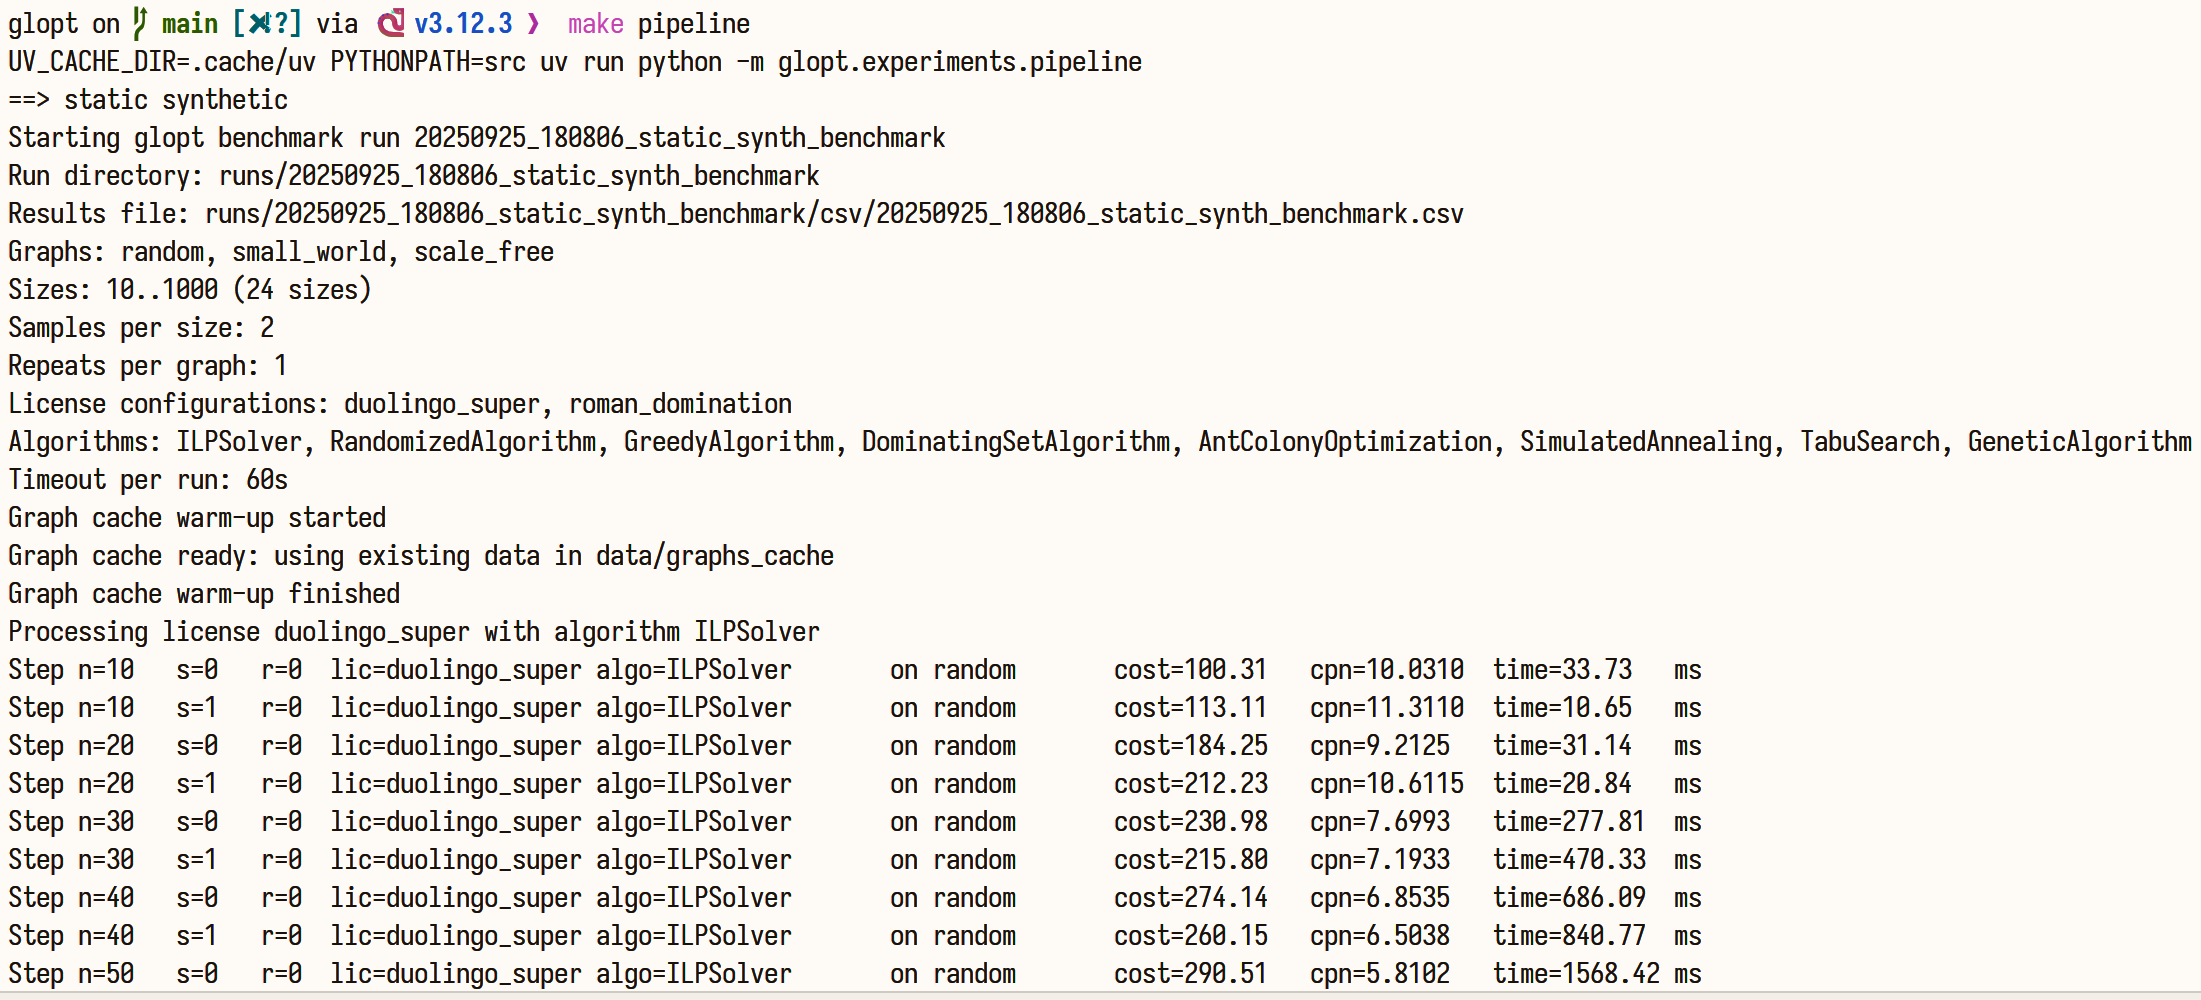
\includegraphics[width=0.95\linewidth]{assets/cli-content.png}
  \caption{Przykładowy przebieg uruchomienia potoku eksperymentalnego z Makefile.}
  \label{fig:cli-content}
\end{figure}

Na początku wyświetlane są informacje o wybranych parametrach uruchomienia, takich jak typ potoku, konfiguracje licencji, lista algorytmów oraz limity czasowe. Następnie rozpoczyna się proces przygotowania grafów. Tworzony jest \textit{magazyn grafów} (cache), który pozwala na wielokrotne wykorzystanie tych samych instancji grafów pomiędzy różnymi algorytmami i konfiguracjami licencji. Dzięki temu nie ma potrzeby generowania grafów od nowa dla każdej próby, co znacząco skraca czas obliczeń, zwłaszcza dla dużych instancji.

Po przygotowaniu grafów wyświetlane są szczegóły dotyczące liczby rozmiarów, próbek i powtórzeń dla każdej instancji. Następnie dla każdej kombinacji licencji i algorytmu prezentowane są postępy obliczeń. Każda iteracja pokazuje podstawowe statystyki, takie jak rozmiar grafu, koszt rozwiązania, koszt na węzeł oraz czas wykonania. Pozwala to na bieżąco monitorować przebieg eksperymentu i szybko wykryć ewentualne anomalie.

\section{Duolingo Super na grafach syntetycznych}

\subsection{Statystyki zbiorcze}
Tabela~\ref{tab:duo-synth-summary} zestawia średnie wartości kosztu licencji na wierzchołek oraz czasu dla licencji Duolingo Super. Solver ILP pozostaje najlepszym punktem odniesienia jakościowego (średni koszt na węzeł 0.445), lecz ma zastosowanie jedynie dla mniejszych instancji. Posiada tyle samo timeoutów co algorytm mrówkowy. Wśród metaheurystyk najniższy koszt na węzeł osiąga właśnie algorytm mrówkowy (0.506), natomiast przeszukiwanie tabu zapewnia najlepszy kompromis kosztu na węzeł i czasu w grupie metod przybliżonych. Algorytm zachłanny i algorytm losowy działają prawie natychmiast, ale tylko pierwszy z nich zachowuje akceptowalny koszt na węzeł (0.548), podczas gdy algorytm losowy pozostaje wyraźnie gorszy jakościowo.

\begin{table}[H]
  \centering
  \caption{Średnie wartości kosztu na węzeł i czasu dla licencji Duolingo Super na grafach syntetycznych.}
  \label{tab:duo-synth-summary}
  \begin{tabular}{lrrr}
    \toprule
    \textbf{Algorytm}     & \textbf{Średni koszt/węzeł} & \textbf{Średni koszt} & \textbf{Średni czas [s]} \\
    \midrule
    Solver ILP            & 0.445                       & 73.83                 & 2.492                    \\
    Algorytm mrówkowy     & 0.506                       & 83.58                 & 5.124                    \\
    Przeszukiwanie tabu   & 0.500                       & 117.80                & 3.298                    \\
    Algorytm genetyczny   & 0.515                       & 118.36                & 1.222                    \\
    Wyżarzanie symulowane & 0.531                       & 120.90                & 0.975                    \\
    Zbiór dominujący      & 0.542                       & 119.97                & 0.017                    \\
    Algorytm zachłanny    & 0.548                       & 121.94                & 0.001                    \\
    Algorytm losowy       & 0.799                       & 179.90                & 0.001                    \\
    \bottomrule
  \end{tabular}
\end{table}


\subsection{Porównanie algorytmów na grafach syntetycznych}

Rysunki~\ref{fig:duo-synth-cost-random}--\ref{fig:duo-synth-cost-small-world} pokazują, że algorytmy dla licencji Duolingo Super osiągają wyniki porównywalne z solverem ILP w przypadku grafów losowych i małoświatowych. Natomiast w przypadku grafów bezskalowych wyniki są zauważalnie gorsze.


\begin{figure}[H]
  \centering
  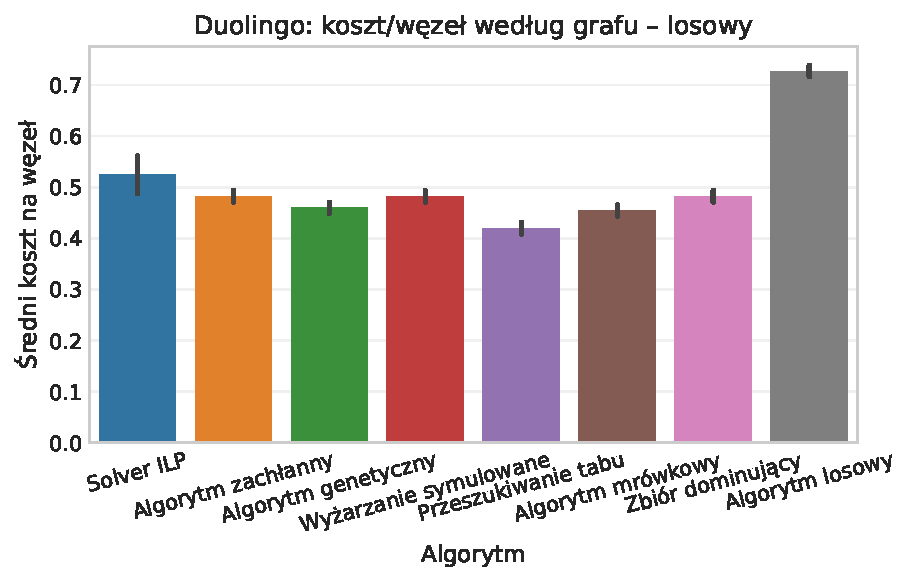
\includegraphics[width=0.65\linewidth]{assets/figures/benchmark/synthetic/duolingo_cost_per_node_by_graph_random.pdf}
  \caption{Koszt na węzeł w zależności od struktury grafu losowej.}
  \label{fig:duo-synth-cost-random}
\end{figure}

\begin{figure}[H]
  \centering
  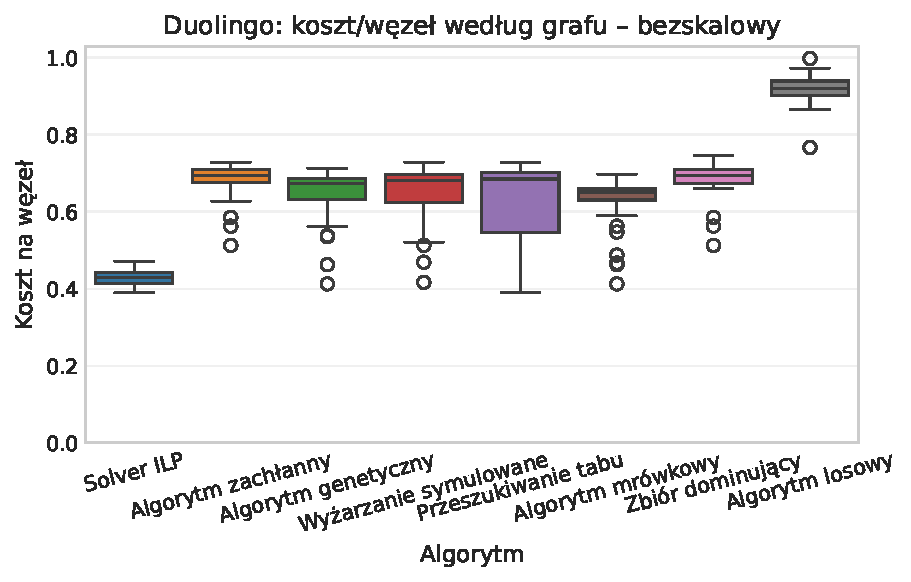
\includegraphics[width=0.65\linewidth]{assets/figures/benchmark/synthetic/duolingo_cost_per_node_by_graph_scale_free.pdf}
  \caption{Koszt na węzeł w zależności od struktury grafu bezskalowej.}
  \label{fig:duo-synth-cost-scale-free}
\end{figure}

\begin{figure}[H]
  \centering
  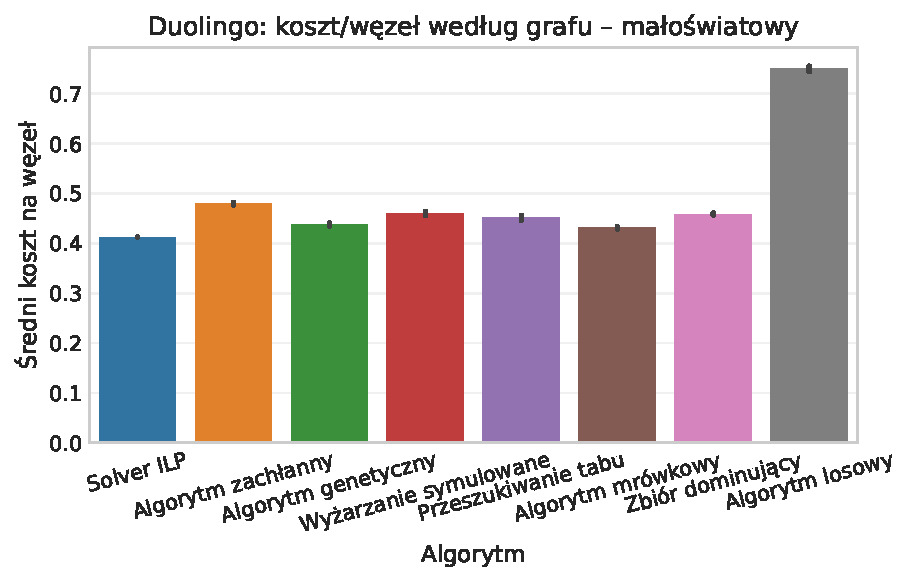
\includegraphics[width=0.65\linewidth]{assets/figures/benchmark/synthetic/duolingo_cost_per_node_by_graph_small_world.pdf}
  \caption{Koszt na węzeł w zależności od struktury grafu małoświatowej.}
  \label{fig:duo-synth-cost-small-world}
\end{figure}

Podobne obserwacje dotyczą czasów wykonania, jak ilustrują rysunki~\ref{fig:duo-synth-time-random}--\ref{fig:duo-synth-time-small-world}. Czasy działania algorytmów są zbliżone dla różnych typów grafów, z wyjątkiem solvera ILP, który średnio działa szybciej na grafach bezskalowych, oraz przeszukiwania tabu, które działa na nich dłużej. Pozostałe algorytmy wykazują porównywalne czasy działania niezależnie od struktury grafu. Tabela~\ref{tab:duo-synth-summary-times} podsumowuje średnie czasów i kosztów na węzeł dla różnych typów grafów.

\begin{figure}[H]
  \centering
  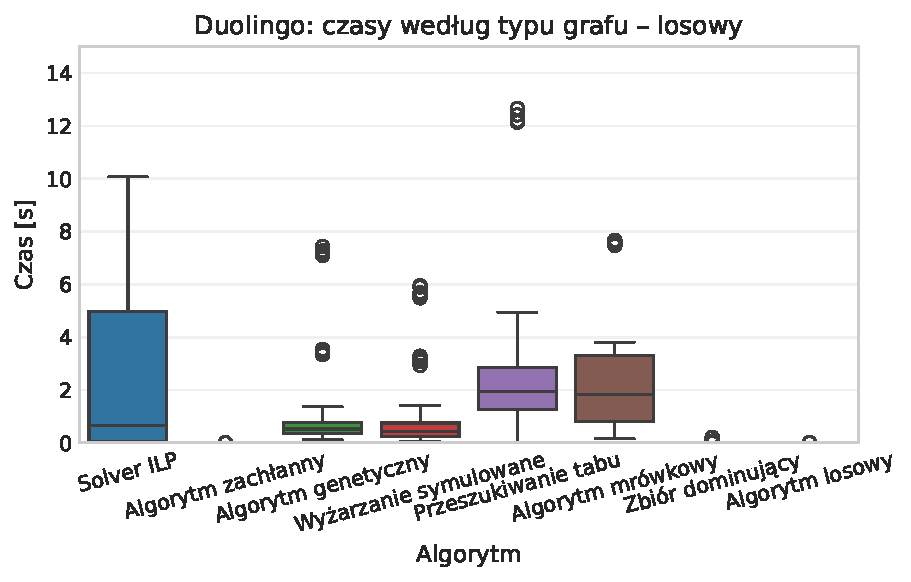
\includegraphics[width=0.65\linewidth]{assets/figures/benchmark/synthetic/duolingo_time_by_graph_random.pdf}
  \caption{Czas wykonania w zależności od struktury grafu losowej.}
  \label{fig:duo-synth-time-random}
\end{figure}

\begin{figure}[H]
  \centering
  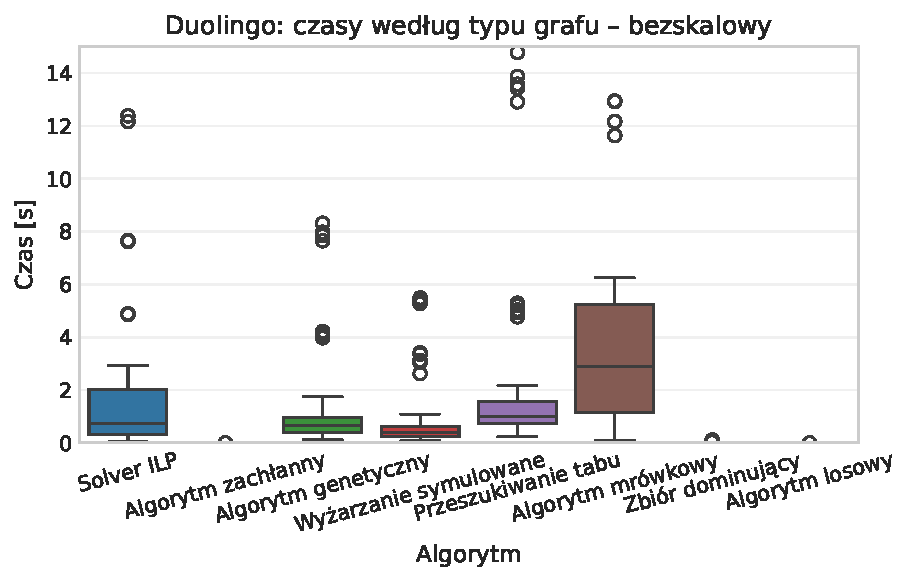
\includegraphics[width=0.65\linewidth]{assets/figures/benchmark/synthetic/duolingo_time_by_graph_scale_free.pdf}
  \caption{Czas wykonania w zależności od struktury grafu bezskalowej.}
  \label{fig:duo-synth-time-scale-free}
\end{figure}

\begin{figure}[H]
  \centering
  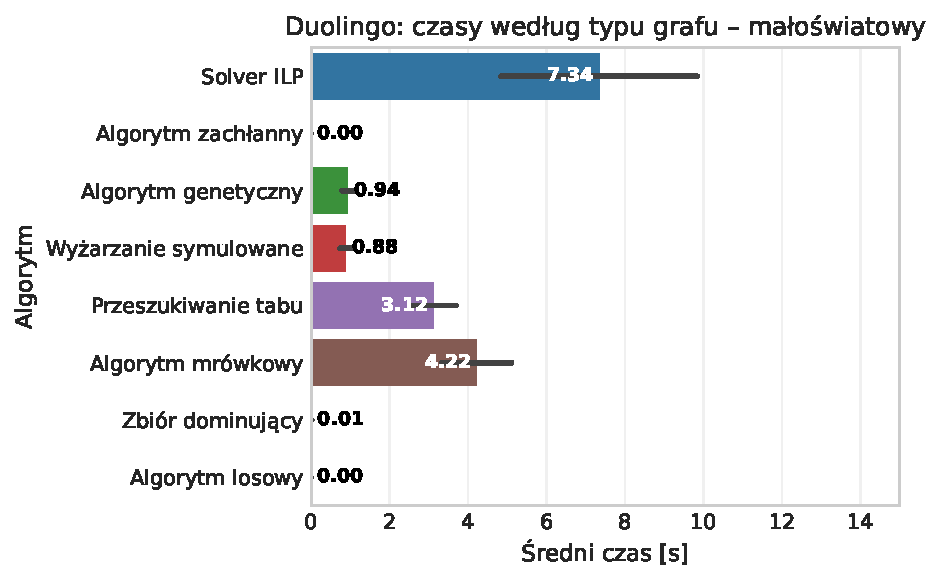
\includegraphics[width=0.65\linewidth]{assets/figures/benchmark/synthetic/duolingo_time_by_graph_small_world.pdf}
  \caption{Czas wykonania w zależności od struktury grafu małoświatowej.}
  \label{fig:duo-synth-time-small-world}
\end{figure}

\begin{table}[H]
  \centering
  \caption{Średnie koszty i czasy na węzeł dla różnych typów grafów (Duolingo Super i dominowanie rzymskie).}
  \label{tab:duo-synth-summary-times}
  \begin{tabular}{lcccc}
    \toprule
    \textbf{Licencja}    & \textbf{Typ grafu} & \textbf{Śr. koszt/węzeł} & \textbf{Śr. czas [s]} \\
    \midrule
    Duolingo Super       & Bezskalowy         & 0.661                    & 1.655                 \\
    Duolingo Super       & Losowy             & 0.502                    & 1.598                 \\
    Duolingo Super       & Małoświatowy       & 0.495                    & 1.346                 \\
    Dominowanie rzymskie & Bezskalowy         & 0.490                    & 0.913                 \\
    Dominowanie rzymskie & Losowy             & 0.344                    & 0.815                 \\
    Dominowanie rzymskie & Małoświatowy       & 0.409                    & 1.544                 \\
    \bottomrule
  \end{tabular}
\end{table}

Z powyższych danych wynika, że dominowanie rzymskie osiąga niższy koszt na węzeł we wszystkich typach grafów syntetycznych. Największą przewagę wykazuje w grafach losowych (różnica 0.158), następnie w bezskalowych (0.171), a najmniejszą w małoświatowych (0.086). Pod względem czasów wykonania Duolingo Super charakteryzuje się dłuższymi czasami w strukturach bezskalowych i losowych, jednak w grafach małoświatowych jest nieco szybszy od dominowania rzymskiego. Struktura bezskalowa okazuje się najkosztowniejsza dla obu schematów licencjonowania, podczas gdy grafy małoświatowe oferują najbardziej korzystny stosunek kosztu do wydajności obliczeniowej. Przewaga kosztowa dominowania rzymskiego wynika naturalnie z tego, że stosunek ceny licencji grupowej do indywidualnej dla dominowania rzymskiego jest niższy niż dla Duolingo Super.


\section{Duolingo Super na grafach rzeczywistych}
W analizie grafów ego z serwisu Facebook pominięto obserwacje, w których solver ILP nie zakończył pracy przed limitem czasu (18 przypadków). Dodatkowo odnotowano 8 timeoutów algorytmu mrówkowego i 6 przypadków w przeszukiwaniu tabu; pozostałe uruchomienia zakończyły się sukcesem.

\begin{table}[H]
  \centering
  \caption{Statystyki kosztu i czasu dla licencji Duolingo Super na grafach rzeczywistych.}
  \label{tab:duo-real-alg}
  \begin{tabular}{lrrr}
    \toprule
    \textbf{Algorytm}     & \textbf{Średni koszt} & \textbf{Śr. koszt/węzeł} & \textbf{Śr. czas [s]} \\
    \midrule
    Algorytm mrówkowy     & 83.58                 & 0.506                    & 5.124                 \\
    Zbiór dominujący      & 119.97                & 0.542                    & 0.017                 \\
    Algorytm genetyczny   & 118.36                & 0.515                    & 1.222                 \\
    Algorytm zachłanny    & 121.94                & 0.548                    & 0.001                 \\
    Algorytm losowy       & 179.90                & 0.799                    & 0.001                 \\
    Wyżarzanie symulowane & 120.90                & 0.531                    & 0.975                 \\
    Przeszukiwanie tabu   & 117.80                & 0.500                    & 3.298                 \\
    \bottomrule
  \end{tabular}
\end{table}
Tabela~\ref{tab:duo-real-alg} pokazuje, że zarówno przeszukiwanie tabu, jak i algorytm mrówkowy zachowują przewagę kosztową nad heurystykami losowymi i zachłannymi, choć okupują ją dłuższym czasem działania.

\subsection{Skalowanie i jakość}

Rysunek~\ref{fig:duo-real-size} pokazuje, że wraz ze wzrostem liczby wierzchołków koszt na węzeł rośnie umiarkowanie, przy czym przeszukiwanie tabu utrzymuje najniższe wartości, a algorytm mrówkowy plasuje się tuż za nim. Czasy działania wszystkich metod mieszczą się w przedziale do kilku sekund i rosną łagodnie wraz z rozmiarem grafu; algorytm zachłanny nadal pozostaje niemal natychmiastowy i stanowi dobry punkt startowy dla metaheurystyk. Dodatkowo tabela~\ref{tab:duo-real-size-table} zbiera średnie wartości (TabuSearch) dla kolejnych rozmiarów sieci ego i pokazuje, że koszt na węzeł utrzymuje się w przedziale 1.8--2.5 przy czasie rosnącym od ułamka sekundy do około 5.5~s dla największych grafów.

\begin{figure}[H]
  \centering
  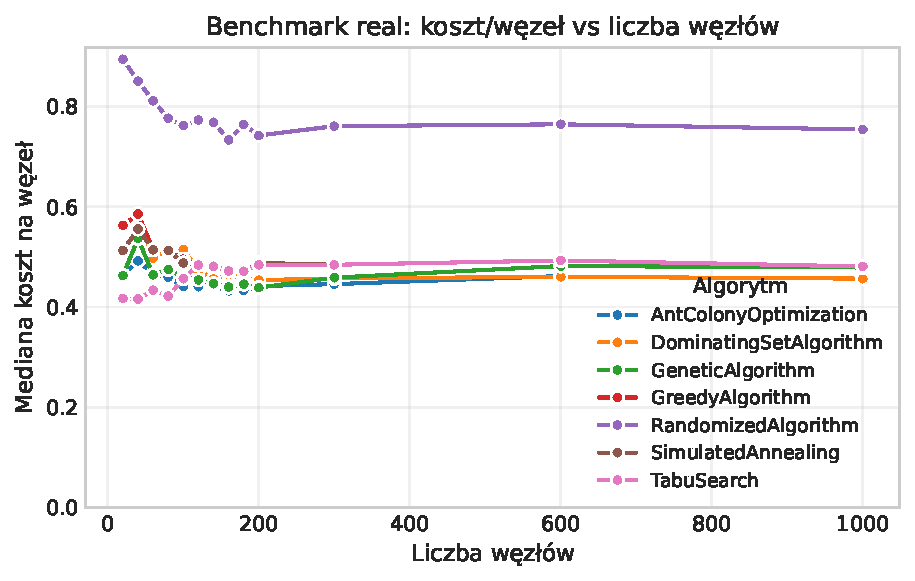
\includegraphics[width=0.48\linewidth]{assets/figures/benchmark/real/cost_per_node_vs_nodes.pdf}
  \hfill
  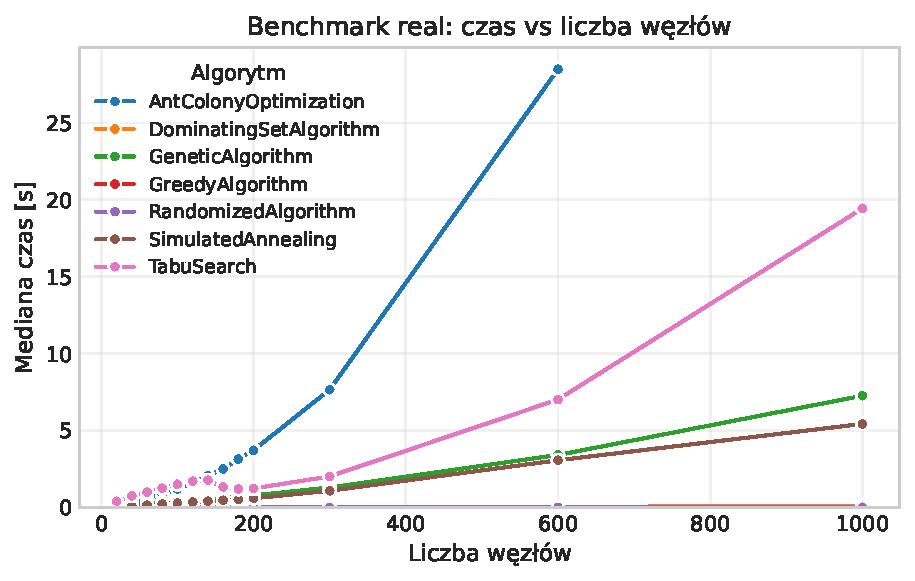
\includegraphics[width=0.48\linewidth]{assets/figures/benchmark/real/time_vs_nodes.pdf}
  \caption{Koszt na węzeł i czas wykonania licencji Duolingo Super w funkcji liczby wierzchołków (grafy ego Facebook).}
  \label{fig:duo-real-size}
\end{figure}

\begin{table}[H]
  \centering
  \caption{Średni koszt licencji na węzeł i czas (przeszukiwanie tabu) względem liczby wierzchołków w sieciach ego Facebook.}
  \label{tab:duo-real-size-table}
  \begin{tabular}{lrr}
    \toprule
    \textbf{Liczba wierzchołków} & \textbf{Śr. koszt/węzeł} & \textbf{Śr. czas [ms]} \\
    \midrule
    53                           & 6.175                    & 2161.349               \\
    62                           & 5.175                    & 3141.926               \\
    151                          & 5.297                    & 6825.722               \\
    169                          & 5.499                    & 8726.145               \\
    225                          & 5.704                    & 12324.041              \\
    334                          & 7.843                    & 32705.396              \\
    535                          & 7.400                    & 58557.464              \\
    \bottomrule
  \end{tabular}
\end{table}


\section{Porównanie z dominowaniem rzymskim}

Porównania z dominowaniem rzymskim ograniczono do wspólnych instancji i algorytmów. Rysunki~\ref{fig:duo-roman-cost}--\ref{fig:duo-roman-license} zestawiają różnice w kosztach, czasach i strukturze licencji, a tabela~\ref{tab:duo-roman-graph} gromadzi średnie według typu grafu syntetycznego.

\begin{table}[H]
  \centering
  \caption{Średnie czasu i kosztu na węzeł według typu grafu (wspólne instancje).}
  \label{tab:duo-roman-graph}
  \begin{tabular}{lcccc}
    \toprule
    \multirow{2}{*}{\textbf{Typ grafu}} & \multicolumn{2}{c}{\textbf{Duolingo Super}} & \multicolumn{2}{c}{\textbf{Dominowanie rzymskie}}                                            \\
                                        & \textbf{Czas [s]}                           & \textbf{Koszt/węzeł}                              & \textbf{Czas [s]} & \textbf{Koszt/węzeł} \\
    \midrule
    Losowy                              & 1.598                                       & 0.502                                             & 0.815             & 0.344                \\
    Bezskalowy                          & 1.655                                       & 0.661                                             & 0.913             & 0.490                \\
    Małoświatowy                        & 1.346                                       & 0.495                                             & 1.544             & 0.409                \\
    \bottomrule
  \end{tabular}
\end{table}

Dominowanie rzymskie zapewnia niższy koszt na węzeł we wszystkich porównywanych rodzinach grafów. Największa różnica dotyczy struktur losowych, gdzie przewaga wynosi ok.~0.16 punktu (32\%). W sieciach bezskalowych różnica maleje do 0.17, natomiast w małoświatowych do 0.09. Czasy wykonania są porównywalne, przy lekkiej przewadze Duolingo Super w grafach małoświatowych, ale dominowanie rzymskie jest szybsze w grafach losowych i bezskalowych. Rysunek~\ref{fig:duo-roman-cost} ilustruje te obserwacje dla pełnego rozkładu, a rysunek~\ref{fig:duo-roman-time} prezentuje analogiczne dane czasowe. Warto zauważyć, że wyższe koszty na węzeł w przypadku Duolingo Super wynikają z ograniczeń w opłacalności licencji grupowych. Licencja grupowa jest około 2.1 razy droższa od indywidualnej, co oznacza, że opłaca się ją tworzyć dopiero dla grup liczących co najmniej trzy osoby (właściciel i dwóch sąsiadów). W efekcie liczba licencji indywidualnych w Duolingo Super jest większa, co przekłada się na wyższy średni koszt na węzeł w porównaniu do dominowania rzymskiego.

\begin{figure}[H]
  \centering
  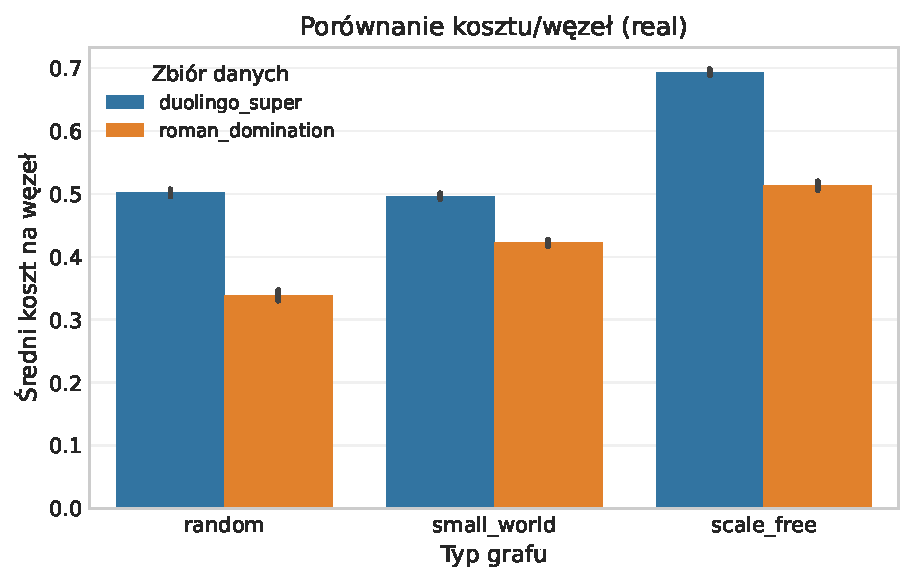
\includegraphics[width=0.6\linewidth]{assets/figures/benchmark/real/duo_vs_roman_cost_per_node_by_graph.pdf}
  \caption{Koszt na węzeł według typu grafu: porównanie licencji Duolingo Super i dominowania rzymskiego.}
  \label{fig:duo-roman-cost}
\end{figure}

\begin{figure}[H]
  \centering
  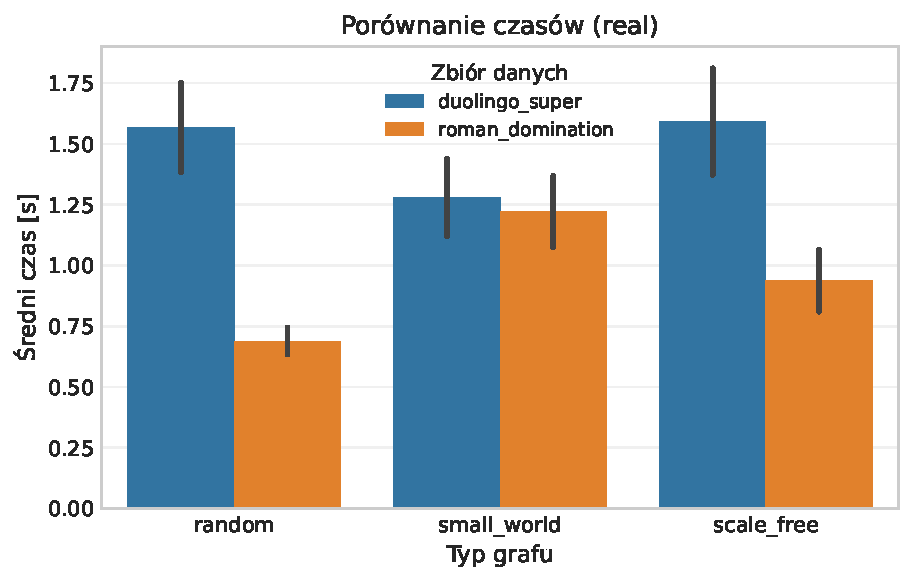
\includegraphics[width=0.6\linewidth]{assets/figures/benchmark/real/duo_vs_roman_time_by_graph.pdf}
  \caption{Czas wykonania według typu grafu: porównanie licencji Duolingo Super i dominowania rzymskiego.}
  \label{fig:duo-roman-time}
\end{figure}

Rysunek~\ref{fig:duo-roman-license} pokazuje, że dominowanie rzymskie charakteryzuje się wyższym stosunkiem licencji grupowych do indywidualnych w porównaniu do Duolingo Super. W przypadku dominowania rzymskiego stosunek ten wynosi około 1.15:1, podczas gdy dla Duolingo Super jest to około 0.88:1.

Różnica ta wynika z faktu, że dominowanie rzymskie nie posiada ograniczenia maksymalnej pojemności grupy licencyjnej. W przypadku Duolingo Super, gdy grupa osiąga maksymalną pojemność, dodatkowi użytkownicy, którzy mogliby do niej należeć, są zmuszeni do zakupu licencji indywidualnych. W pełnym zbiorze danych, obejmującym trzy typy grafów syntetycznych, zaobserwowano 137690 licencji w Duolingo Super, z czego 73176 (53.15\%) to licencje indywidualne. W przypadku dominowania rzymskiego, dzięki braku ograniczeń pojemności grup, liczba licencji indywidualnych jest proporcjonalnie niższa.

\begin{figure}[H]
  \centering
  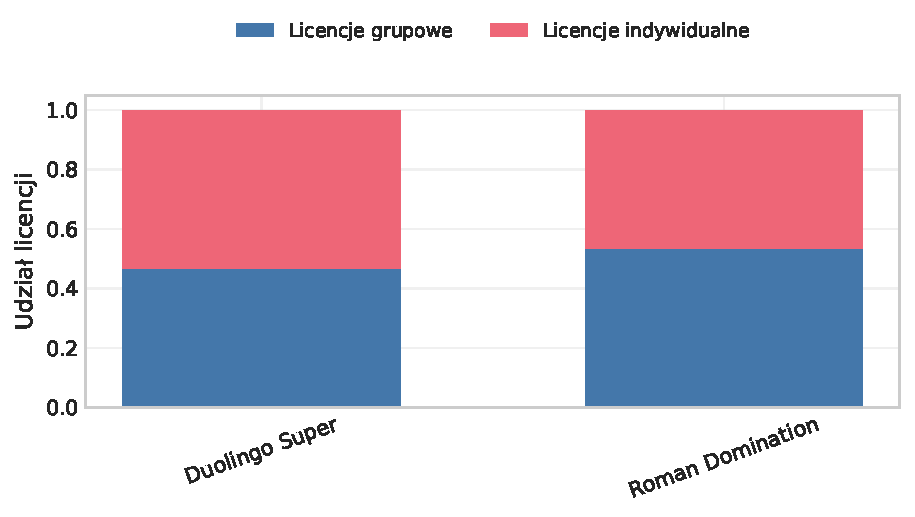
\includegraphics[width=0.6\linewidth]{assets/figures/benchmark/synthetic/license_mix_duo_vs_roman.pdf}
  \caption{Struktura wykorzystania licencji: porównanie licencji Duolingo Super i dominowania rzymskiego.}
  \label{fig:duo-roman-license}
\end{figure}

\section{Wnioski}

Przeprowadzone eksperymenty pokazują, że schemat licencjonowania Duolingo Super zapewnia stabilne i powtarzalne wyniki. Spośród badanych metod najlepiej wypadły algorytm mrówkowy oraz przeszukiwanie tabu. Algorytm mrówkowy osiąga najniższy koszt na węzeł w grupie metaheurystyk, lecz wymaga dłuższego czasu działania. Przeszukiwanie tabu pozwala uzyskać porównywalną jakość i jednocześnie zachowuje lepszy kompromis między kosztem a czasem obliczeń.

Solver ILP stanowi wartościowe odniesienie jakościowe, jednak jego zastosowanie jest ograniczone do mniejszych instancji ze względu na częste przekroczenia limitu czasu. Proste heurystyki, takie jak algorytm zachłanny czy losowy, działają bardzo szybko, ale ich wyniki są wyraźnie gorsze jakościowo.

Wyniki potwierdzają również znaczenie struktury grafu. W przypadku grafów losowych i małoświatowych możliwe jest osiągnięcie rezultatów zbliżonych do solvera ILP, natomiast grafy bezskalowe okazały się trudniejsze i generowały wyższe koszty. Skalowanie pokazane na rysunku~\ref{fig:duo-real-size} dowodzi, że przeszukiwanie tabu zachowuje niskie koszty na węzeł nawet przy rosnącej liczbie wierzchołków, a czasy działania rosną umiarkowanie.

Porównanie z dominowaniem rzymskim wskazuje, że schemat ten osiąga niższy koszt na węzeł we wszystkich typach grafów. Wynika to z większego udziału licencji grupowych i niższego kosztu jednostkowego. Duolingo Super charakteryzuje się natomiast krótszym czasem działania w grafach małoświatowych oraz większą stabilnością wyników.

\chapter{Symulacja dynamiczna}\label{chap:dynamic}

\section{Założenia i konfiguracja}

Eksperymenty dynamiczne wykonano w tym samym środowisku obliczeniowym co testy statyczne. Każda symulacja obejmuje 30 kroków, a po każdej mutacji sieci algorytmy otrzymują maksymalnie 45~s na ponowne zbilansowanie licencji. Analizowano dwie konfiguracje licencyjne -- Duolingo Super oraz dominowanie rzymskie.

\subsection{Poziomy intensywności mutacji}

Warianty \emph{low}, \emph{med} oraz \emph{high} różnią się prawdopodobieństwami modyfikacji wierzchołków i krawędzi (tab.~\ref{tab:dyn-mutation-levels}).

\begin{table}[H]
  \centering
  \caption{Parametry intensywności mutacji w symulacji dynamicznej.}
  \label{tab:dyn-mutation-levels}
  \begin{tabular}{lcccc}
    \toprule
    \textbf{Poziom} & \textbf{Dodawanie węzłów} & \textbf{Usuwanie węzłów} & \textbf{Dodawanie krawędzi} & \textbf{Usuwanie krawędzi} \\
    \midrule
    niski           & 0.02                      & 0.01                     & 0.06                        & 0.04                       \\
    średni          & 0.06                      & 0.04                     & 0.18                        & 0.12                       \\
    wysoki          & 0.12                      & 0.08                     & 0.30                        & 0.20                       \\
  \end{tabular}
\end{table}

\subsection{Scenariusze realistyczne}

Dodatkowo zbadano trzy bardziej realistyczne profile ewolucji sieci. Wszystkie operują na tych samych limitach liczby dodawanych/usuwanych elementów co warianty syntetyczne, różnią się jednak mechanizmem wyboru sąsiedztwa. Wariant \emph{pref\_triadic} tworzy nowe wierzchołki z preferencyjnym przyłączaniem (stopień +1) i zamyka trójkąty w sąsiedztwie bieżących wierzchołków. Wariant \emph{pref\_pref} stosuje preferencyjne przyłączanie zarówno do węzłów, jak i krawędzi. Wreszcie \emph{rand\_rewire} łączy losowe dodawanie węzłów z przekształcaniem istniejących krawędzi w stylu Wattsa--Strogatza, gdzie losowa zamiana końców krawędzi zachodzi z prawdopodobieństwem 0,1 na operację.

\section{Algorytm zachłanny}

W tym wariancie algorytm zachłanny w każdym kroku symulacji buduje rozwiązanie całkowicie od zera. Stanowi to dolną granicę narzutu czasowego dla metod bez pamięci oraz bazowy punkt odniesienia jakości, do którego porównujemy bardziej zaawansowane metaheurystyki korzystające z rozwiązań z poprzedniego kroku.

\subsection{Zestawienie dla wszystkich mutacji}
Tabela~\ref{tab:greedy-cold-summary} zestawia średni koszt na węzeł i średni czas na krok dla sześciu badanych profili mutacji: trzech syntetycznych oraz trzech realistycznych. Wszystkie czasy mieszczą się w przedziale 0.5--1.8 ms na krok, a średni koszt na węzeł oscyluje wokół 0.46--0.48.

\begin{table}[H]
  \centering
  \caption{Algorytm zachłanny: średni koszt na węzeł oraz średni czas na krok dla wszystkich wariantów mutacji.}
  \label{tab:greedy-cold-summary}
  \begin{tabular}{lcc}
    oprule
    extbf{Metoda mutacji} & \textbf{Koszt/węzeł (mean)} & \textbf{Średni czas [s]} \\
    \midrule
    high                  & 0.48009                     & 0.00159                  \\
    low                   & 0.47983                     & 0.00165                  \\
    med                   & 0.47491                     & 0.00181                  \\
    pref\_pref            & 0.46371                     & 0.000835                 \\
    pref\_triadic         & 0.46787                     & 0.000535                 \\
    rand\_rewire          & 0.47556                     & 0.000833                 \\
    \bottomrule
  \end{tabular}
\end{table}

Algorytm zachłanny jest bardzo szybki (sub-milisekundowy do \SI{1.8}{\ms}), co potwierdza jego przydatność jako lekki baseline czasowy w środowisku dynamicznym. Warianty realistyczne sprzyjają nieco niższym kosztom: \texttt{pref\_pref} osiąga najniższy średni koszt (0.464), a \texttt{pref\_triadic} jest jednocześnie najszybszy (\SI{0.000535}{\s}). Wariant \texttt{rand\_rewire} jest trudniejszy (0.476), ale pozostaje bardzo szybki czasowo.

Różnice kosztu dla mutacji syntetycznych są niewielkie (0.475--0.480), natomiast czasy są wyższe niż w profilach realistycznych, szczególnie dla \texttt{med/high}. Wskazuje to, że bardziej lokalne, realistyczne przekształcenia struktury grafu są łatwiejsze do obsłużenia. Mediany czasów są niższe niż średnie (np. \texttt{pref\_pref}: mediana \SI{0.00058}{\s} vs średnia \SI{0.00083}{\s}, \emph{n}=930; \texttt{pref\_triadic}: \SI{0.00046}{\s} vs \SI{0.00053}{\s}, \emph{n}=744), co sugeruje długi ogon rzadkich, nieco wolniejszych kroków. Analogiczne zjawisko obserwujemy w mutacjach syntetycznych (\emph{n}=1116 na wariant).

\section{Wyniki na mutacjach syntetycznych}
\subsection{Metaheurystyki}

Tabela~\ref{tab:dyn-synth-warm} przedstawia zbiorcze wyniki dla różnych metod mutacji. Średni koszt na węzeł jest bardzo zbliżony dla wszystkich poziomów intensywności, z jedynie nieznacznym wzrostem dla wariantu \texttt{high}. Sugeruje to, że algorytmy są w stanie skutecznie adaptować się do zmian w topologii sieci.

Średni czas wykonania rośnie wraz z intensywnością mutacji. Wariant \texttt{low} jest najszybszy, podczas gdy \texttt{high} wymaga najwięcej czasu na ponowne zbilansowanie. Jest to naturalna konsekwencja faktu, że większa liczba modyfikacji grafu (dodawanie/usuwanie węzłów i krawędzi) stanowi większe wyzwanie obliczeniowe dla algorytmów optymalizacyjnych. Mimo to, różnice w czasach nie są drastyczne, co świadczy o dobrej skalowalności zastosowanych metod.

\begin{table}[H]
  \centering
  \caption{Wyniki dla różnych metod mutacji.}
  \label{tab:dyn-synth-warm}
  \begin{tabular}{lcc}
    \toprule
    \textbf{Metoda mutacji} & \textbf{Średni koszt} & \textbf{Średni czas [s]} \\
    \midrule
    high                    & 0.4893                & 3.169                    \\
    med                     & 0.4850                & 3.075                    \\
    low                     & 0.4852                & 2.878                    \\
    \bottomrule
  \end{tabular}
\end{table}

\subsection{Profil kosztu i czasu w czasie}
Jako przykład ewolucji kosztu i czasu w krokach symulacji wybrano algorytm genetyczny. Rysunki~\ref{fig:dyn-synth-genetic-cost} i~\ref{fig:dyn-synth-genetic-time} przedstawiają odpowiednio przebieg kosztu na węzeł oraz czasu wykonania w zależności od kroku symulacji dla różnych poziomów intensywności mutacji.

Dla wariantu \texttt{high} można zaobserwować niewielkie, lecz zauważalne wahania średniego kosztu na węzeł, które nie są tak widoczne w przypadku wariantów \texttt{low} i \texttt{med}. Jeśli chodzi o czasy wykonania, dla każdego z trzech wariantów widoczne są zbliżone wahania w trakcie trwania symulacji.

\begin{figure}[H]
  \centering
  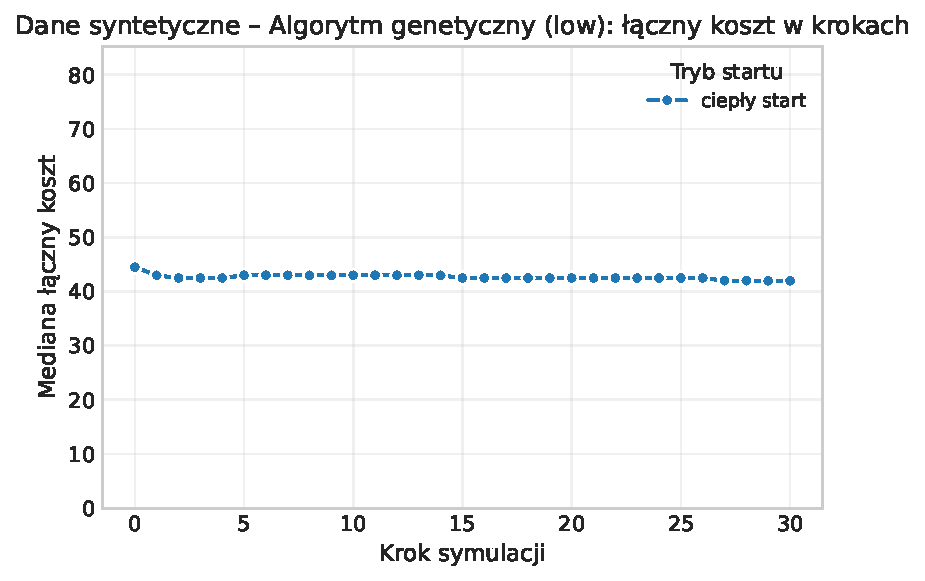
\includegraphics[width=0.32\linewidth]{assets/figures/dynamic/synthetic/synthetic_algorytm_genetyczny_cost_over_steps_low.pdf}
  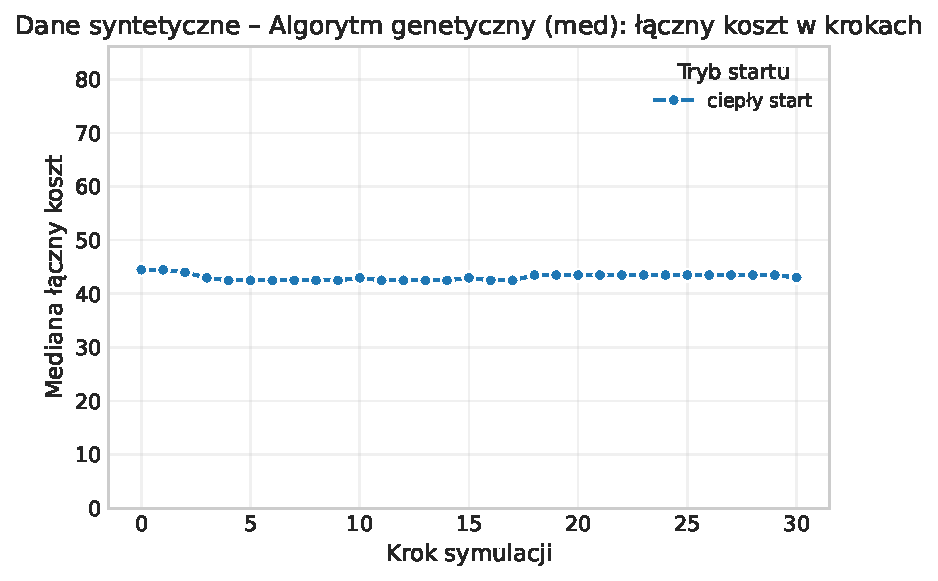
\includegraphics[width=0.32\linewidth]{assets/figures/dynamic/synthetic/synthetic_algorytm_genetyczny_cost_over_steps_med.pdf}
  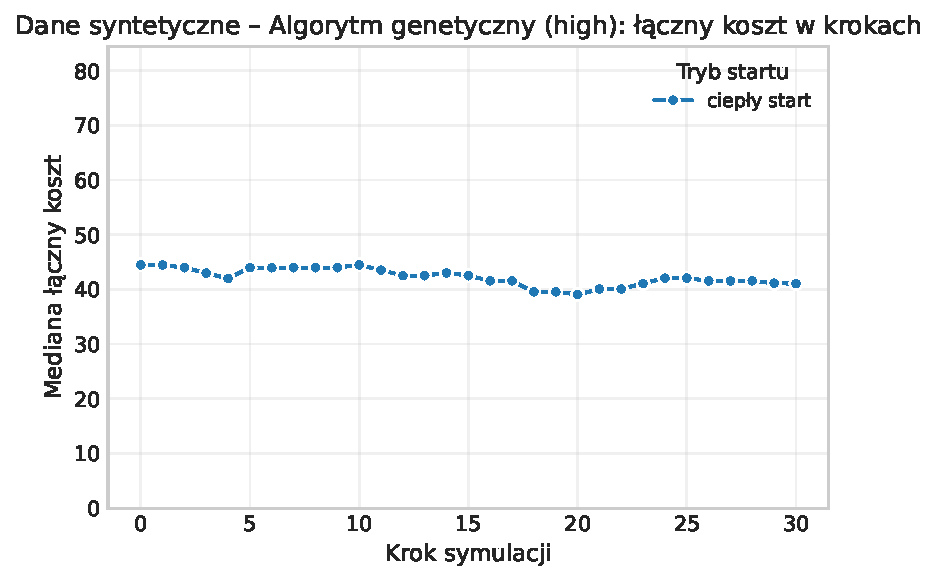
\includegraphics[width=0.32\linewidth]{assets/figures/dynamic/synthetic/synthetic_algorytm_genetyczny_cost_over_steps_high.pdf}
  \caption{Algorytm genetyczny -- koszt na węzeł w funkcji kroku (warianty low/med/high).}
  \label{fig:dyn-synth-genetic-cost}
\end{figure}

\begin{figure}[H]
  \centering
  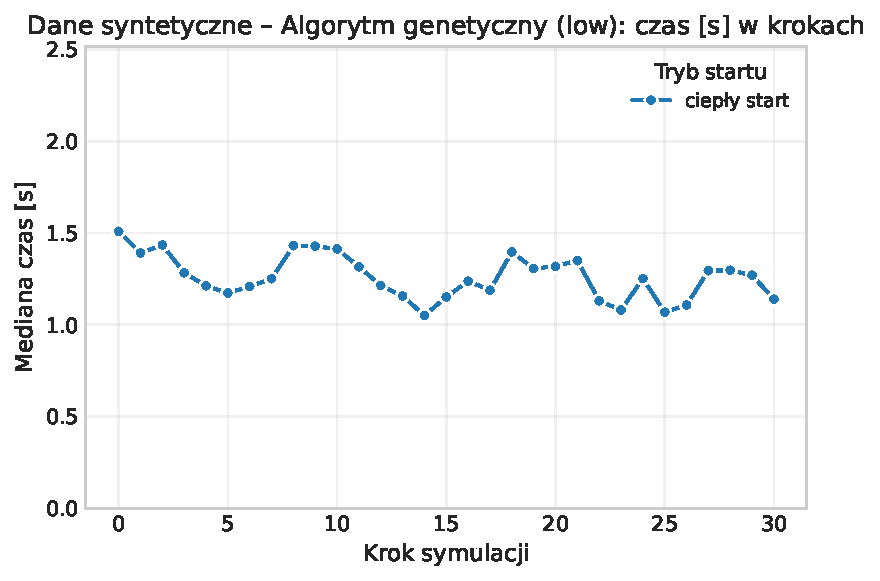
\includegraphics[width=0.32\linewidth]{assets/figures/dynamic/synthetic/synthetic_algorytm_genetyczny_time_over_steps_low.pdf}
  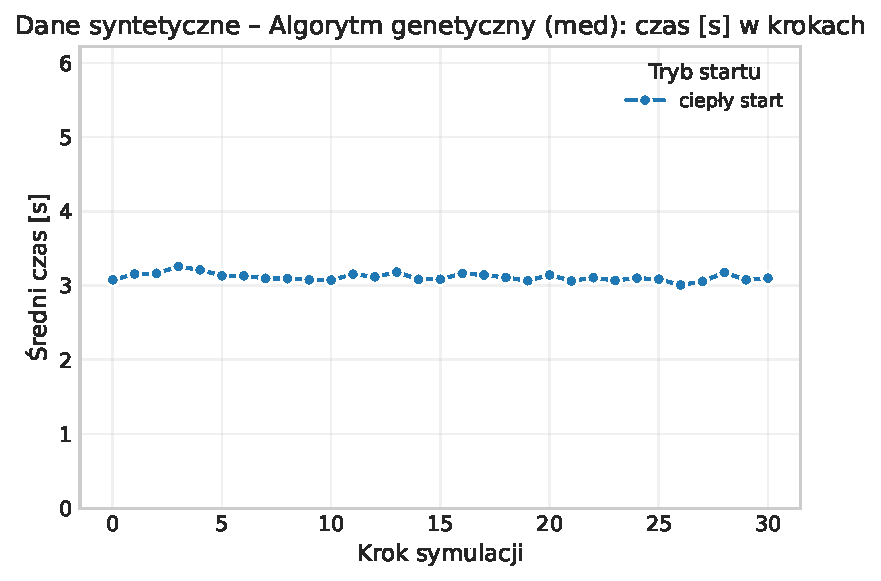
\includegraphics[width=0.32\linewidth]{assets/figures/dynamic/synthetic/synthetic_algorytm_genetyczny_time_over_steps_med.pdf}
  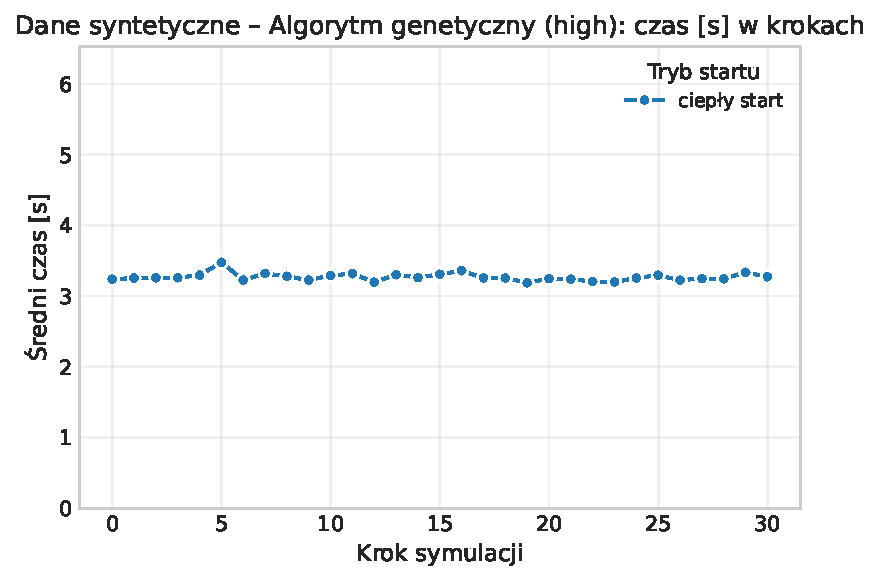
\includegraphics[width=0.32\linewidth]{assets/figures/dynamic/synthetic/synthetic_algorytm_genetyczny_time_over_steps_high.pdf}
  \caption{Algorytm genetyczny -- czas wykonania w funkcji kroku (warianty low/med/high).}
  \label{fig:dyn-synth-genetic-time}
\end{figure}

\section{Wyniki na mutacjach realistycznych}

Tabela~\ref{tab:dyn-real-warm} przedstawia zbiorcze wyniki dla scenariuszy realistycznych. Wariant \texttt{pref\_triadic} wyróżnia się najkrótszym średnim czasem wykonania (poniżej 1 sekundy), przy zachowaniu kosztu na poziomie zbliżonym do wariantu \texttt{pref\_pref}. Scenariusz \texttt{rand\_rewire} okazał się najtrudniejszy -- charakteryzuje się zarówno najwyższym średnim kosztem, jak i najdłuższym czasem przetwarzania.

\begin{table}[H]
  \centering
  \caption{Wyniki dla różnych metod mutacji w scenariuszach realistycznych.}
  \label{tab:dyn-real-warm}
  \begin{tabular}{lcc}
    \toprule
    \textbf{Metoda mutacji} & \textbf{Średni koszt} & \textbf{Średni czas [s]} \\
    \midrule
    pref\_pref              & 0.4699                & 1.743                    \\
    pref\_triadic           & 0.4704                & 0.896                    \\
    rand\_rewire            & 0.4855                & 1.908                    \\
    \bottomrule
  \end{tabular}
\end{table}

\subsection{Wybrane algorytmy i metody mutacji}
Poniżej wybrano kilka par algorytmów i metod mutacji, które pokazują różne kompromisy. Dla porównania uwzględniono również dwie mutacje syntetyczne. Nie są to zawsze najlepsze jakościowo konfiguracje, ale dobrze ilustrują różne scenariusze.

\begin{table}[H]
  \centering
  \caption{Wybrane pary algorytmów i metod mutacji (różne kompromisy).}
  \label{tab:dyn-synth-selected-best}
  \begin{tabular}{llcc}
    \toprule
    \textbf{Algorytm}     & \textbf{Metoda} & \textbf{Koszt/węzeł} & \textbf{Śr. czas [s]} \\
    \midrule
    Solver ILP            & pref\_triadic   & 0.362                & 1.525                 \\
    Solver ILP            & rand\_rewire    & 0.390                & 2.553                 \\
    Algorytm genetyczny   & pref\_triadic   & 0.409                & 0.615                 \\
    Algorytm genetyczny   & high            & 0.429                & 3.269                 \\
    Przeszukiwanie tabu   & pref\_triadic   & 0.413                & 1.470                 \\
    Przeszukiwanie tabu   & high            & 0.447                & 6.454                 \\
    Algorytm mrówkowy     & pref\_pref      & 0.417                & 6.906                 \\
    Algorytm mrówkowy     & pref\_triadic   & 0.424                & 3.002                 \\
    Wyżarzanie symulowane & pref\_triadic   & 0.460                & 0.555                 \\
    Algorytm zachłanny    & pref\_pref      & 0.464                & 0.001                 \\
    Zbiór dominujący      & pref\_triadic   & 0.457                & 0.005                 \\
    Algorytm losowy       & pref\_pref      & 0.754                & 0.001                 \\
    \bottomrule
  \end{tabular}
\end{table}

Solver ILP osiąga najniższe koszty, ale wymaga około 1.5--2.6 sekundy na krok. Algorytm genetyczny dobrze sprawdza się przy zmianach klastrowych (\texttt{pref\_triadic}), oferując niski koszt i czas około 0.6 sekundy. Jednak przy intensywnych mutacjach (\texttt{high}) staje się wyraźnie wolniejszy i droższy. Z kolei wyżarzanie symulowane jest szybkie (około pół sekundy) i stabilne, ale jakościowo ustępuje bardziej zaawansowanym metodom.

Przeszukiwanie tabu korzysta z lokalności zmian, osiągając sensowny koszt i czas około 1.5 sekundy przy \texttt{pref\_triadic}. Jednak przy intensywnych mutacjach (\texttt{high}) czas wzrasta do około 6.5 sekundy, a koszt również rośnie. Algorytm mrówkowy zapewnia bardzo dobrą jakość przy \texttt{pref\_pref}, ale działa najwolniej. Przejście na \texttt{pref\_triadic} prawie podwaja szybkość kosztem niewielkiego pogorszenia jakości.

Heurystyki szybkie, takie jak algorytm zachłanny (około 1 ms) i zbiór dominujący (około 5 ms), są bardzo efektywne. Zbiór dominujący zwykle osiąga niższy koszt niż zachłanny, co czyni go dobrym wyborem przy ograniczeniach czasowych. Mutacje klastrowe (\texttt{pref\_triadic}, \texttt{pref\_pref}) pomagają wszystkim algorytmom utrzymać niski koszt i krótszy czas. Natomiast \texttt{rand\_rewire} i wariant \texttt{high} zwiększają zarówno koszt, jak i czas.

\subsection{Ewolucja kosztów w czasie}
Pełne przebiegi dla algorytmu genetycznego pokazano na rys.~\ref{fig:dyn-real-genetic-cost}--\ref{fig:dyn-real-genetic-time}. Łączenie preferencyjnego przyłączania z triadycznym domykaniem sprzyja utrzymaniu najniższych kosztów, natomiast wariant z losowym przełączaniem krawędzi prowadzi do wolniejszej stabilizacji. Analizując koszt na węzeł (Rys. \ref{fig:dyn-real-genetic-cost}), można zauważyć, że dla każdego z typów mutacji przebiega on podobnie, oscylując wokół zbliżonego poziomu.

Z kolei, patrząc na czas wykonania (Rys. \ref{fig:dyn-real-genetic-time}), widać, że dla wariantu \texttt{rand\_rewire} występują największe wahania, co sugeruje większą niestabilność w procesie optymalizacji. Warianty \texttt{pref\_triadic} i \texttt{pref\_pref} charakteryzują się bardziej stabilnym czasem wykonania.

\begin{figure}[H]
  \centering
  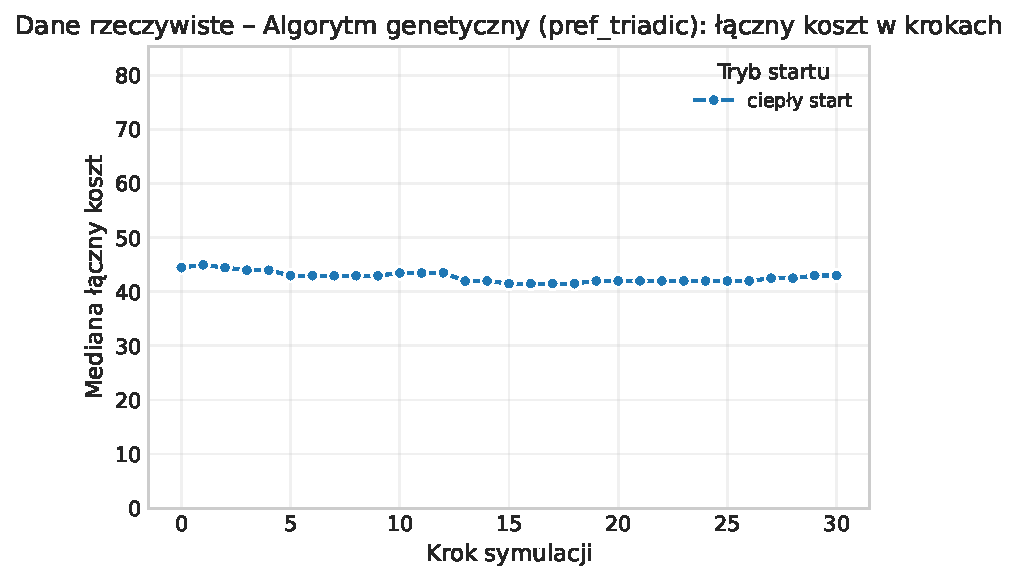
\includegraphics[width=0.32\linewidth]{assets/figures/dynamic/real/real_algorytm_genetyczny_cost_over_steps_pref_triadic.pdf}
  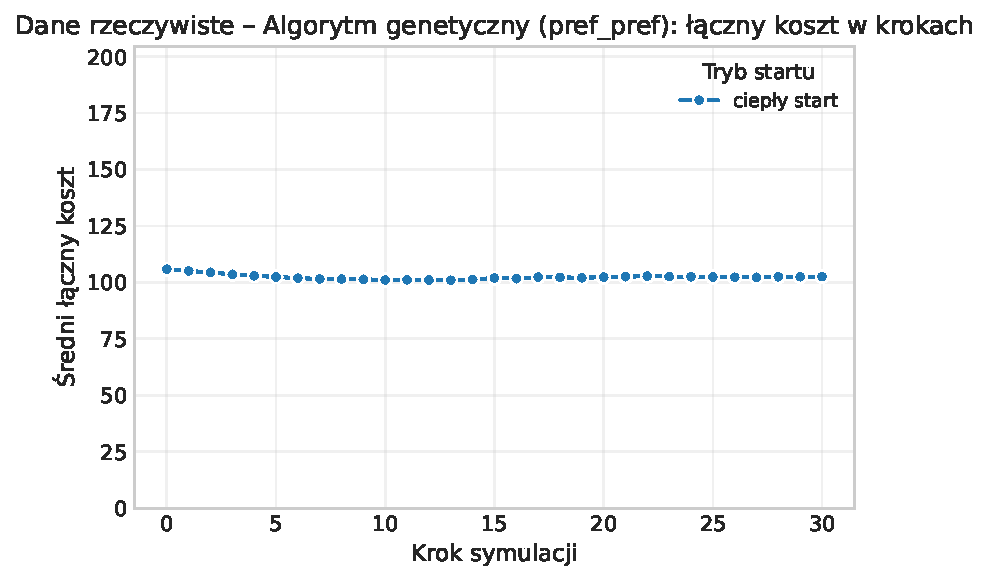
\includegraphics[width=0.32\linewidth]{assets/figures/dynamic/real/real_algorytm_genetyczny_cost_over_steps_pref_pref.pdf}
  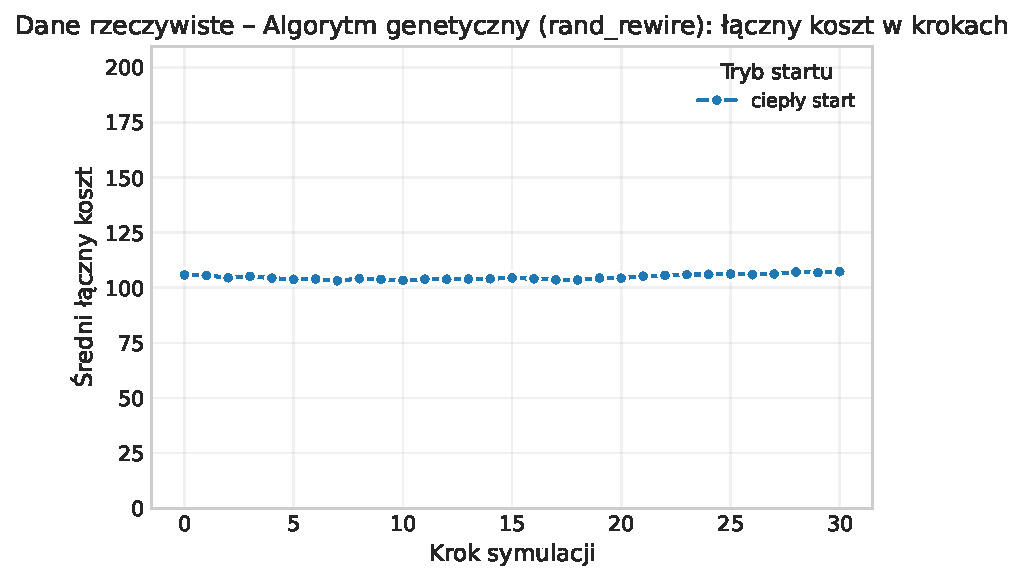
\includegraphics[width=0.32\linewidth]{assets/figures/dynamic/real/real_algorytm_genetyczny_cost_over_steps_rand_rewire.pdf}
  \caption{Algorytm genetyczny -- koszt na węzeł w wariantach realistycznych.}
  \label{fig:dyn-real-genetic-cost}
\end{figure}

\begin{figure}[H]
  \centering
  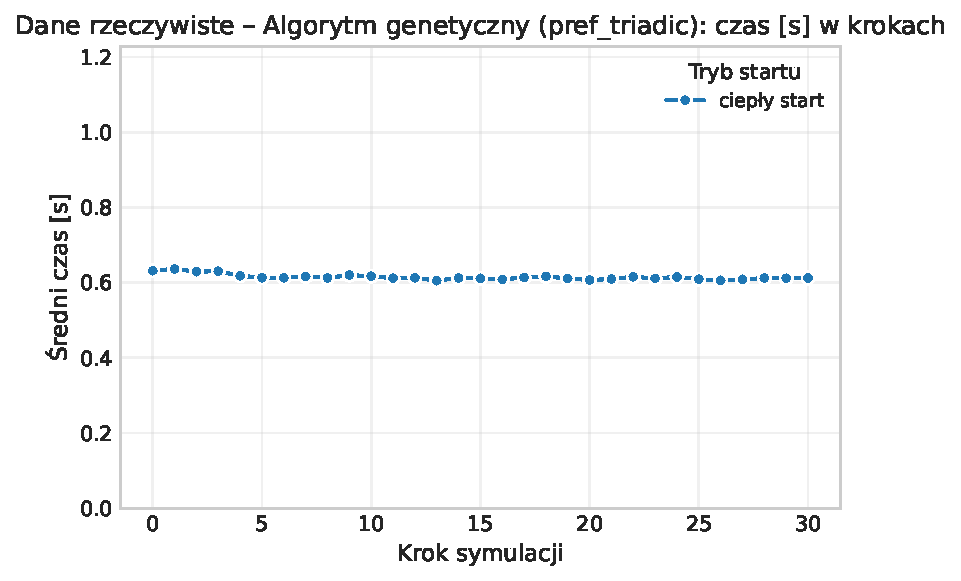
\includegraphics[width=0.32\linewidth]{assets/figures/dynamic/real/real_algorytm_genetyczny_time_over_steps_pref_triadic.pdf}
  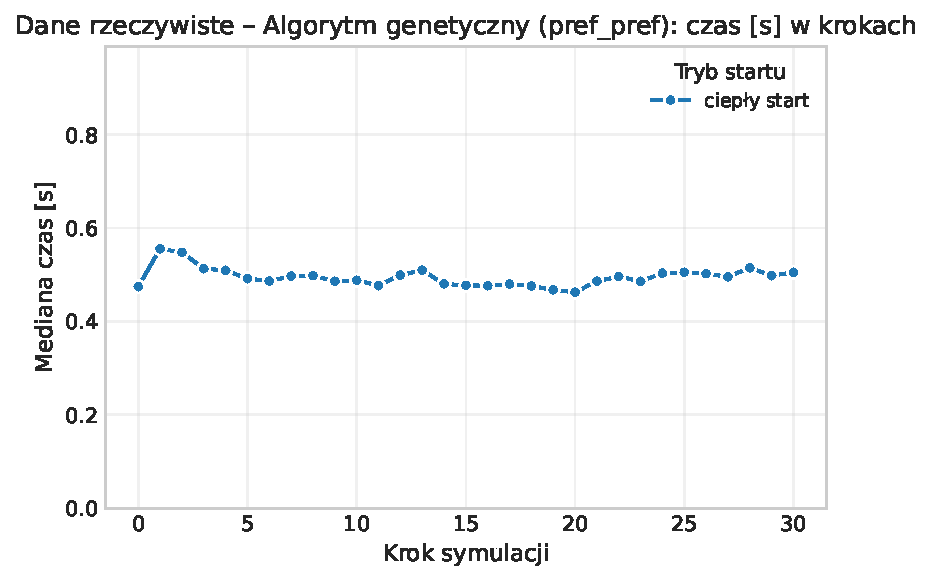
\includegraphics[width=0.32\linewidth]{assets/figures/dynamic/real/real_algorytm_genetyczny_time_over_steps_pref_pref.pdf}
  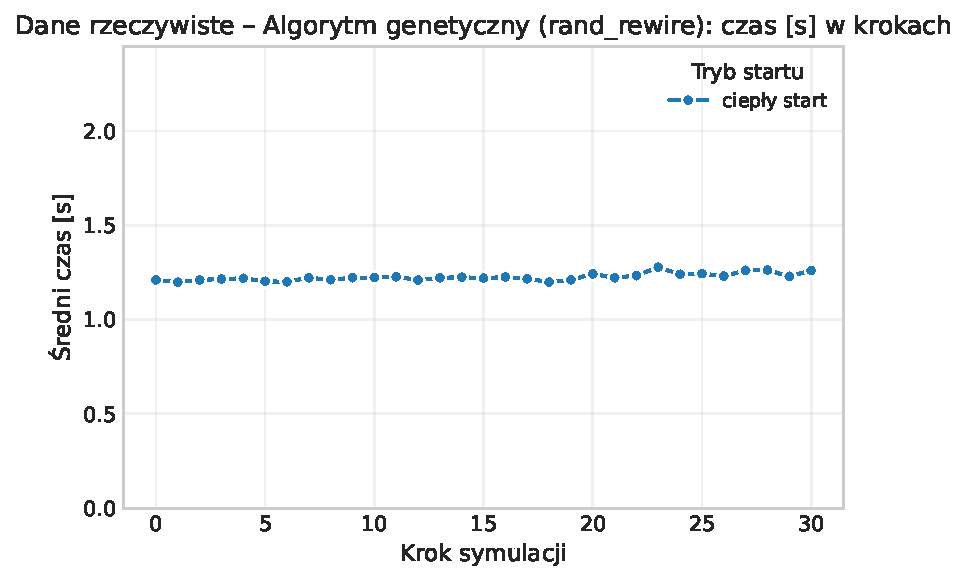
\includegraphics[width=0.32\linewidth]{assets/figures/dynamic/real/real_algorytm_genetyczny_time_over_steps_rand_rewire.pdf}
  \caption{Algorytm genetyczny -- czas wykonania w wariantach realistycznych.}
  \label{fig:dyn-real-genetic-time}
\end{figure}

\subsection{Wnioski}
Analiza dynamiczna pokazała, że metaheurystyki radzą sobie z adaptacją do zmian w sieci i utrzymaniem jakości rozwiązań bez potrzeby liczenia wszystkiego od nowa.

Zwiększenie intensywności zmian, szczególnie w testach syntetycznych, powodowało wydłużenie czasu potrzebnego na zrównoważenie. Algorytmy takie jak przeszukiwanie tabu miały też tendencję do wzrostu kosztu przy bardzo dużych zmianach.

Metody zmian oparte na preferencyjnym dołączaniu i zamykaniu trójkątów (\texttt{pref\_triadic}) tworzyły struktury, które łatwiej było optymalizować. Przekładało się to na niższy koszt i krótszy czas działania większości algorytmów.

Solver ILP nadal dawał najlepsze wyniki pod względem jakości, ale działał dość długo. Z kolei proste metody, jak algorytm zachłanny, działały bardzo szybko, ale dawały gorsze wyniki. Metaheurystyki były czymś pośrodku, oferując dobry balans między jakością a czasem.

Reasumując, symulacje dynamiczne potwierdziły, że adaptacyjne zarządzanie licencjami za pomocą metaheurystyk ma sens. Pozwalają one na utrzymanie stabilnego kosztu w zmieniającej się sieci, przy akceptowalnym kompromisie między jakością a czasem.

\chapter{Rozszerzenia modelu licencjonowania}\label{chap:extensions}

W niniejszym rozdziale przedstawiono analizę rozszerzeń podstawowego modelu licencjonowania, które uwzględniają różne konfiguracje cenowe oraz ograniczenia pojemności planów grupowych. Badania obejmują osiem wariantów licencyjnych inspirowanych rzeczywistymi ofertami platform takich jak Duolingo, Spotify czy Netflix. Rozdział zawiera szczegółową analizę wpływu poszczególnych parametrów na efektywność optymalizacji oraz porównanie kosztów i czasów wykonania algorytmów w różnych konfiguracjach.

\section{Przegląd badanych wariantów}
Oprócz bazowych konfiguracji rozważono osiem rozszerzeń licencyjnych, które różnią się wielokrotnością kosztu licencji grupowej względem indywidualnej. Warianty Duolingo Super obejmują plany, w których koszt licencji grupowej wynosi odpowiednio dwukrotność, czterokrotność i pięciokrotność ceny licencji indywidualnej, przy zachowaniu stałej pojemności grupy (6 osób). Podobnie, w przypadku dominowania rzymskiego analizowano konfiguracje, w których koszt licencji grupowej wynosi $p$-krotność ceny indywidualnej, dla $p \in \{3, 4, 5\}$. Dwa ostatnie warianty odnoszą się do rzeczywistych ofert: Spotify oferuje plan Duo (pojemność 2) jako wariant pośredni między licencją indywidualną a rodzinną, natomiast Netflix oferuje plany dla 1, 2 lub 4 osób.

Przedstawione w tabelach wartości stanowią statystyki zagregowane dla danej konfiguracji licencyjnej. Oznacza to, że średnie koszty na węzeł oraz średnie czasy obliczeń zostały obliczone na podstawie wyników wszystkich zastosowanych algorytmów oraz wszystkich typów grafów uwzględnionych w eksperymentach. Tabele nie odnoszą się zatem do pojedynczego algorytmu czy sieci, lecz prezentują uśrednione efekty całej grupy uruchomień dla danej konfiguracji licencji.


\subsection{Warianty rodziny Duolingo}
Na rys.~\ref{fig:ext-duolingo-cost} przedstawiono mediany kosztu na węzeł dla konfiguracji, w których koszt licencji grupowej wynosi odpowiednio dwukrotność (\texttt{duolingo\_p\_2}), czterokrotność (\texttt{duolingo\_p\_4}) oraz pięciokrotność (\texttt{duolingo\_p\_5}) ceny licencji indywidualnej. Wyniki wskazują, że wyższe mnożniki prowadzą do wzrostu kosztu na węzeł, co wynika z częstszej selekcji licencji indywidualnych przy wyższych kosztach planów grupowych. W przypadku konfiguracji \texttt{duolingo\_p\_4} oznacza to, że sens kupna licencji grupowej pojawia się dopiero dla grup liczących 4 lub więcej osób, ponieważ dopiero wtedy koszt licencji grupowej jest równy lub niższy niż koszt czterech licencji indywidualnych.

Szczegółowe statystyki dla wariantów Duolingo zebrano w tabeli~\ref{tab:ext-duolingo-stats}. Wzrost mnożnika ceny grupowej z 2 do 5 powoduje wzrost średniego kosztu na węzeł o 77\% (z 0.554 do 0.982) oraz wydłużenie średniego czasu obliczeń o 47\% (z 0.637 s do 0.938 s).

\begin{table}[H]
  \centering
  \caption{Statystyki dla wariantów Duolingo (benchmark statyczny).}
  \label{tab:ext-duolingo-stats}
  \begin{tabular}{llrrrr}
    \toprule
    \textbf{Konfiguracja}   & \textbf{Metryka} & \textbf{Średnia} & \textbf{Odch. std.} & \textbf{Min} & \textbf{Max} \\
    \midrule
    \texttt{duolingo\_p\_2} & Czas [s]         & 0.637            & 1.210               & 0.000        & 7.722        \\
                            & Koszt całkowity  & 49.152           & 39.533              & 8.000        & 177.000      \\
                            & Koszt/węzeł      & 0.554            & 0.152               & 0.340        & 1.000        \\
    \midrule
    \texttt{duolingo\_p\_4} & Czas [s]         & 0.677            & 1.483               & 0.000        & 11.075       \\
                            & Koszt całkowity  & 76.815           & 59.581              & 14.000       & 259.000      \\
                            & Koszt/węzeł      & 0.860            & 0.171               & 0.680        & 1.520        \\
    \midrule
    \texttt{duolingo\_p\_5} & Czas [s]         & 0.938            & 2.721               & 0.000        & 26.589       \\
                            & Koszt całkowity  & 87.855           & 67.852              & 17.000       & 300.000      \\
                            & Koszt/węzeł      & 0.982            & 0.198               & 0.840        & 1.820        \\
    \bottomrule
  \end{tabular}
\end{table}



Analiza rozrzutu wartości w tabeli~\ref{tab:ext-duolingo-stats} pokazuje stabilność wyników. Odchylenie standardowe dla kosztu na węzeł pozostaje na niskim poziomie (0.152--0.198), co wskazuje na konsekwentność rozwiązań algorytmów w różnych instancjach. Warto zauważyć, że w konfiguracji \texttt{duolingo\_p\_5} odnotowano najwyższy maksymalny czas obliczeń (26.589 s), co może wynikać z większej złożoności problemu przy wyższych kosztach planów grupowych. Zwiększone odchylenie standardowe dla czasów wykonania w tej konfiguracji (2.721 s) sugeruje większą wrażliwość algorytmów na charakterystykę konkretnej instancji sieci.

\begin{figure}[H]
  \centering
  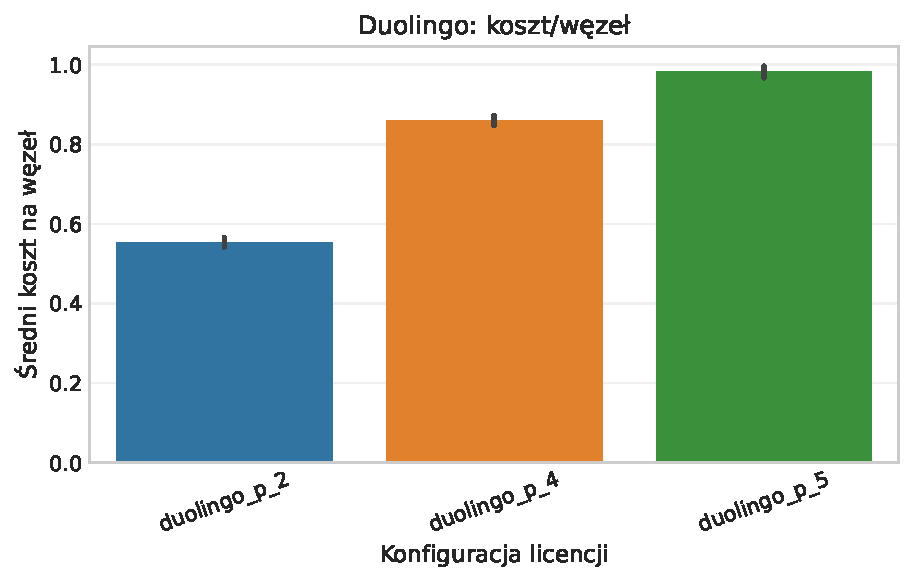
\includegraphics[width=0.6\linewidth]{assets/figures/extensions/static/duolingo_cost_per_node_comparison.pdf}
  \caption{Koszt na węzeł w zależności od planu Duolingo (mediany kluczowych algorytmów).}
  \label{fig:ext-duolingo-cost}
\end{figure}

Zmiana struktury licencji wpływa również na udział planów grupowych. W konfiguracji \texttt{duolingo\_p\_2} ponad połowa przydziałów wykorzystuje licencję grupową, podczas gdy w wariancie \texttt{duolingo\_p\_5} udział grup spada do 24\%, co odzwierciedla rosnący koszt planu grupowego względem licencji indywidualnych.

\subsection{Warianty dominowania rzymskiego}
Na rys.~\ref{fig:ext-roman-cost} przedstawiono mediany kosztu na węzeł dla konfiguracji, w których koszt licencji grupowej wynosi odpowiednio trzykrotność (\texttt{roman\_p\_3}), czterokrotność (\texttt{roman\_p\_4}) oraz pięciokrotność (\texttt{roman\_p\_5}) ceny licencji indywidualnej. Podobnie jak w przypadku planów Duolingo, wyższe mnożniki prowadzą do wzrostu kosztu na węzeł, co wynika z preferencji algorytmów do korzystania z licencji indywidualnych przy wyższych kosztach planów grupowych. Wariant \texttt{roman\_p\_5} charakteryzuje się najwyższym kosztem, co odzwierciedla ograniczoną opłacalność licencji grupowych w tej konfiguracji.

Szczegółowe statystyki dla wariantów dominowania rzymskiego zebrano w tabeli~\ref{tab:ext-roman-stats}. Wzrost mnożnika ceny grupowej z 3 do 5 powoduje wzrost średniego kosztu na węzeł o 37\% (z 0.585 do 0.800) oraz nieznaczne wydłużenie średniego czasu obliczeń (z 0.477 s do 0.493 s).

\begin{table}[H]
  \centering
  \caption{Statystyki dla wariantów dominowania rzymskiego (benchmark statyczny).}
  \label{tab:ext-roman-stats}
  \begin{tabular}{llrrrr}
    \toprule
    \textbf{Konfiguracja} & \textbf{Metryka} & \textbf{Średnia} & \textbf{Odch. std.} & \textbf{Min} & \textbf{Max} \\
    \midrule
    \texttt{roman\_p\_3}  & Czas [s]         & 0.477            & 1.038               & 0.000        & 9.522        \\
                          & Koszt całkowity  & 50.261           & 40.552              & 7.000        & 218.000      \\
                          & Koszt/węzeł      & 0.585            & 0.199               & 0.260        & 1.170        \\
    \midrule
    \texttt{roman\_p\_4}  & Czas [s]         & 0.475            & 1.125               & 0.000        & 9.189        \\
                          & Koszt całkowity  & 60.441           & 48.750              & 9.000        & 259.000      \\
                          & Koszt/węzeł      & 0.701            & 0.232               & 0.340        & 1.400        \\
    \midrule
    \texttt{roman\_p\_5}  & Czas [s]         & 0.493            & 1.289               & 0.000        & 12.314       \\
                          & Koszt całkowity  & 68.995           & 55.987              & 11.000       & 300.000      \\
                          & Koszt/węzeł      & 0.800            & 0.269               & 0.395        & 1.660        \\
    \bottomrule
  \end{tabular}
\end{table}

Zmiana struktury licencji wpływa również na udział planów grupowych (tabela~\ref{tab:ext-license-mix}). W konfiguracji \texttt{roman\_p\_3} udział grup wynosi 43\%, podczas gdy w wariancie \texttt{roman\_p\_5} spada do 24\%. Wyższe koszty planów grupowych prowadzą do preferencji algorytmów w kierunku licencji indywidualnych, co jest zgodne z obserwacjami dla innych rozszerzeń.

\begin{figure}[H]
  \centering
  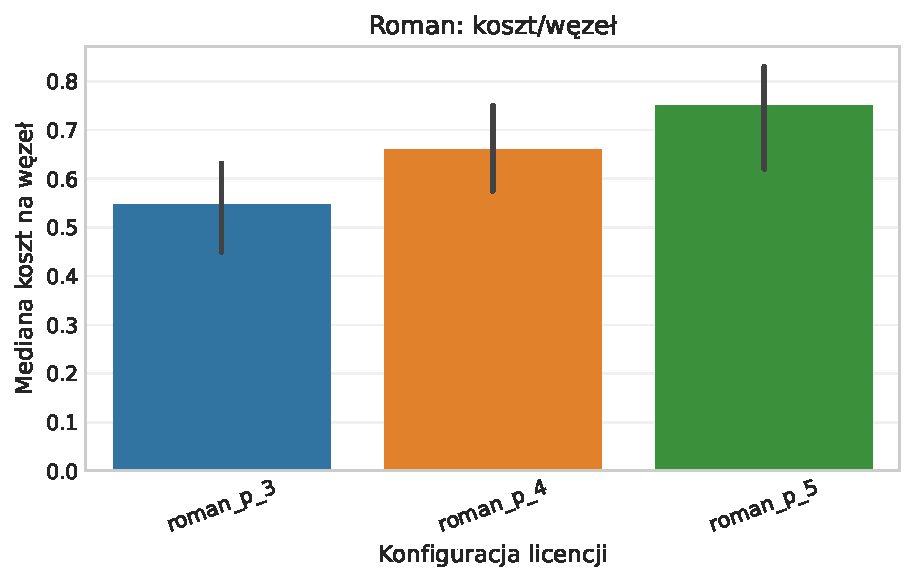
\includegraphics[width=0.6\linewidth]{assets/figures/extensions/static/roman_cost_per_node_comparison.pdf}
  \caption{Koszt na węzeł dla wariantów dominowania rzymskiego.}
  \label{fig:ext-roman-cost}
\end{figure}

\subsection{Spotify i Netflix}

Spotify oferuje plan Duo, przeznaczony dla 2 osób. Umożliwia to efektywne dobieranie użytkowników w pary zamiast tworzenia dużych grup rodzinnych. Tabela~\ref{tab:ext-additional-static} potwierdza, że przeszukiwanie tabu i algorytm genetyczny osiągają najniższe koszty ($0.335$ i $0.400$ na węzeł), uzyskując wyniki niższe niż heurystyka zachłanna.

W przypadku Netflixa plan Standard (również dla 2 osób) stanowi wariant pośredni między licencją indywidualną a planem rodzinnym dla czterech kont, co pozwala metaheurystykom utrzymać koszt w zakresie od $0.60$ do $0.65$ przy czasie poniżej 1~s.

\begin{table}[H]
  \centering
  \caption{Mediany dla konfiguracji Spotify i Netflix.}
  \label{tab:ext-additional-static}
  \begin{tabular}{llrr}
    \toprule
    \textbf{Konfiguracja} & \textbf{Algorytm}   & \textbf{Med. koszt/węzeł} & \textbf{Med. czas [s]} \\
    \midrule
    spotify               & Algorytm zachłanny  & 0.446                     & 0.000                  \\
    spotify               & Algorytm genetyczny & 0.400                     & 0.229                  \\
    spotify               & Algorytm mrówkowy   & 0.391                     & 1.040                  \\
    spotify               & Przeszukiwanie tabu & 0.335                     & 0.958                  \\
    netflix               & Algorytm zachłanny  & 0.682                     & 0.000                  \\
    netflix               & Algorytm genetyczny & 0.650                     & 0.237                  \\
    netflix               & Algorytm mrówkowy   & 0.656                     & 1.289                  \\
    netflix               & Przeszukiwanie tabu & 0.604                     & 0.999                  \\
  \end{tabular}
\end{table}

\begin{figure}[H]
  \centering
  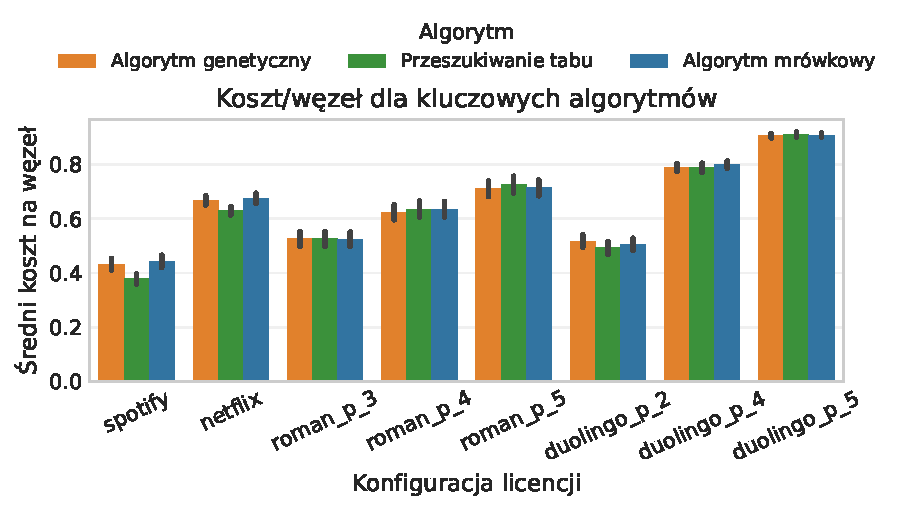
\includegraphics[width=0.6\linewidth]{assets/figures/extensions/static/cost_per_node_by_license_targets.pdf}
  \caption{Koszt na węzeł dla wszystkich rozszerzeń (mediany).}
  \label{fig:ext-license-cost}
\end{figure}


\subsection{Porównanie wszystkich rozszerzeń}

Podstawowe statystyki dla wszystkich konfiguracji zestawiono w tabeli~\ref{tab:ext-overall-static}. W każdym przypadku analizowano ten sam zestaw algorytmów, pomijając obserwacje z przekroczeniem limitu czasu.

\begin{table}[H]
  \centering
  \caption{Statystyki agregowane dla rozszerzeń (benchmark statyczny).}
  \label{tab:ext-overall-static}
  \begin{tabular}{lrr}
    \toprule
    \textbf{Konfiguracja} & \textbf{Śr. koszt/węzeł} & \textbf{Śr. czas [s]} \\
    \midrule
    duolingo\_p\_2        & 0.554                    & 0.637                 \\
    duolingo\_p\_4        & 0.860                    & 0.677                 \\
    duolingo\_p\_5        & 0.982                    & 0.938                 \\
    spotify               & 0.479                    & 0.547                 \\
    netflix               & 0.729                    & 0.623                 \\
    roman\_p\_3           & 0.585                    & 0.477                 \\
    roman\_p\_4           & 0.701                    & 0.475                 \\
    roman\_p\_5           & 0.800                    & 0.493                 \\
  \end{tabular}
\end{table}

Analiza agregowanych statystyk w tabeli~\ref{tab:ext-overall-static} ujawnia wyraźne różnice między rodzinami konfiguracji. W przypadku wariantów Duolingo obserwuje się silną korelację między mnożnikiem ceny grupowej a kosztem na węzeł -- wzrost parametru z 2 do 5 prowadzi do zwiększenia kosztu o 77\% (z 0.554 do 0.982). Jednocześnie czas obliczeń wydłuża się o 47\%, co wskazuje na rosnącą złożoność problemu przy wyższych kosztach planów grupowych.

Warianty dominowania rzymskiego charakteryzują się większą stabilnością obliczeniową, z czasami wykonania w zakresie 0.477--0.493~s niezależnie od parametru $p$. Wzrost kosztu na węzeł jest bardziej umiarkowany (37\% przy wzroście $p$ z 3 do 5), co sugeruje odmienną strukturę przestrzeni rozwiązań w porównaniu z planami Duolingo.

Najkorzystniejszy stosunek kosztu do wydajności obliczeniowej wykazuje konfiguracja Spotify (0.479 kosztu na węzeł przy 0.547~s), co potwierdza skuteczność wprowadzenia planu pośredniego (Duo) między licencjami indywidualnymi a rodzinnymi. Netflix zajmuje pozycję pośrednią z kosztem 0.729 na węzeł, pozostając jednak konkurencyjny pod względem czasu obliczeń (0.623~s).

\subsection{Analiza wpływu liczby użytkowników na koszty}

Struktura wykorzystania licencji zmienia się istotnie (tabela~\ref{tab:ext-license-mix}). W Spotify licencje grupowe odpowiadają za 64\% przydziałów (plan Duo + rodzina), podczas gdy w wariancie \texttt{duolingo\_p\_5} udział grup spada do 24\%. W Netflixie większość przydziałów to plany Standard/Premium (udział 68\%).

\begin{table}[H]
  \centering
  \caption{Udział licencji grupowych i indywidualnych (benchmark statyczny).}
  \label{tab:ext-license-mix}
  \begin{tabular}{lrr}
    \toprule
    \textbf{Konfiguracja} & \textbf{Udział grup} & \textbf{Udział indywidualnych} \\
    \midrule
    duolingo\_p\_2        & 0.56                 & 0.44                           \\
    duolingo\_p\_4        & 0.34                 & 0.66                           \\
    duolingo\_p\_5        & 0.24                 & 0.76                           \\
    spotify               & 0.64                 & 0.36                           \\
    netflix               & 0.68                 & 0.32                           \\
    roman\_p\_3           & 0.43                 & 0.57                           \\
    roman\_p\_4           & 0.34                 & 0.66                           \\
    roman\_p\_5           & 0.24                 & 0.76                           \\
    \bottomrule
  \end{tabular}
\end{table}


\section{Rozszerzenia w środowisku dynamicznym}

W środowisku dynamicznym przeanalizowano te same osiem konfiguracji rozszerzeń, stosując identyczną metodologię jak w benchmarku statycznym. Każda konfiguracja została przetestowana na 272 instancjach dynamicznych, obejmujących różne rozmiary sieci i scenariusze zmian.

\subsection{Statystyki agregowane}

Tabela~\ref{tab:ext-dynamic-family} przedstawia statystyki zagregowane według rodzin konfiguracji. Warianty Duolingo charakteryzują się najwyższymi kosztami średnimi (73.83 na instancję) oraz najdłuższymi czasami wykonania (0.97~s), co wynika z konieczności rozważania licencji o pojemności 6 osób. Problem dominowania rzymskiego wykazuje umiarkowane koszty (59.96) przy porównywalnym czasie obliczeń (0.85~s). Konfiguracje rzeczywistych serwisów -- Spotify i Netflix -- osiągają najkorzystniejsze wyniki, z najniższymi kosztami odpowiednio 43.32 i 66.58.

\begin{table}[H]
  \centering
  \caption{Statystyki zagregowane według rodzin konfiguracji (benchmark dynamiczny).}
  \label{tab:ext-dynamic-family}
  \begin{tabular}{lrrrr}
    \toprule
    \textbf{Rodzina} & \textbf{Śr. czas [s]} & \textbf{Śr. koszt całk.} & \textbf{Śr. koszt/węzeł} & \textbf{Liczba obs.} \\
    \midrule
    Duolingo         & 0.969                 & 73.83                    & 0.792                    & 3265                 \\
    Roman            & 0.853                 & 59.96                    & 0.661                    & 3408                 \\
    Netflix          & 0.891                 & 66.58                    & 0.714                    & 1074                 \\
    Spotify          & 0.881                 & 43.32                    & 0.467                    & 1088                 \\
    \bottomrule
  \end{tabular}
\end{table}

\subsection{Porównanie szczegółowe konfiguracji}

Tabela~\ref{tab:ext-dynamic-detailed} zawiera szczegółowe statystyki dla wszystkich wariantów rozszerzeń. W rodzinie Duolingo obserwuje się wyraźny wzrost kosztu na węzeł wraz ze wzrostem mnożnika ceny grupowej -- od 0.539 w konfiguracji \texttt{duolingo\_p\_2} do 0.980 w \texttt{duolingo\_p\_5}. Podobną tendencję wykazują warianty dominowania rzymskiego, gdzie koszt rośnie z 0.554 (\texttt{roman\_p\_3}) do 0.763 (\texttt{roman\_p\_5}).

\begin{table}[H]
  \centering
  \caption{Szczegółowe statystyki dla rozszerzeń (benchmark dynamiczny).}
  \label{tab:ext-dynamic-detailed}
  \begin{tabular}{lrrrr}
    \toprule
    \textbf{Konfiguracja} & \textbf{Śr. czas [s]} & \textbf{Śr. koszt całk.} & \textbf{Śr. koszt/węzeł} & \textbf{Liczba obs.} \\
    \midrule
    duolingo\_p\_2        & 0.939                 & 50.22                    & 0.539                    & 1088                 \\
    duolingo\_p\_4        & 0.987                 & 80.17                    & 0.855                    & 1073                 \\
    duolingo\_p\_5        & 0.980                 & 90.94                    & 0.980                    & 1104                 \\
    spotify               & 0.881                 & 43.32                    & 0.467                    & 1088                 \\
    netflix               & 0.891                 & 66.58                    & 0.714                    & 1074                 \\
    roman\_p\_3           & 0.798                 & 50.30                    & 0.554                    & 1136                 \\
    roman\_p\_4           & 0.930                 & 60.41                    & 0.666                    & 1136                 \\
    roman\_p\_5           & 0.829                 & 69.18                    & 0.763                    & 1136                 \\
    \bottomrule
  \end{tabular}
\end{table}

Konfiguracja Spotify potwierdza swoją przewagę osiągając najniższy koszt na węzeł (0.467), co stanowi wynik o 13\% lepszy niż w najbliższej konfiguracji \texttt{roman\_p\_3}. Plan Duo umożliwia efektywne parowanie użytkowników, co przekłada się na oszczędności w całym spektrze rozmiarów sieci. Netflix zajmuje pozycję pośrednią z kosztem 0.714 na węzeł, pozostając konkurencyjny wobec wariantów o wysokich mnożnikach.

\subsection{Struktura wykorzystania licencji}

Analiza składu licencji (tabela~\ref{tab:ext-dynamic-license-mix}) ujawnia znaczące różnice w strategiach przydzielania. Konfiguracje o niskich mnożnikach (\texttt{duolingo\_p\_2}, \texttt{spotify}) preferują licencje grupowe, osiągając udział odpowiednio 55\% i 63\%. W przeciwieństwie do tego, wysokie koszty planów grupowych w \texttt{duolingo\_p\_5} i \texttt{roman\_p\_5} prowadzą do dominacji licencji indywidualnych (76\% i 76\% udziału).

\begin{table}[H]
  \centering
  \caption{Struktura wykorzystania licencji (benchmark dynamiczny).}
  \label{tab:ext-dynamic-license-mix}
  \begin{tabular}{lrr}
    \toprule
    \textbf{Konfiguracja} & \textbf{Udział grup [\%]} & \textbf{Udział indywidualnych [\%]} \\
    \midrule
    duolingo\_p\_2        & 55.4                      & 44.6                                \\
    duolingo\_p\_4        & 33.3                      & 66.7                                \\
    duolingo\_p\_5        & 23.0                      & 77.0                                \\
    spotify               & 63.0                      & 37.0                                \\
    netflix               & 66.8                      & 33.2                                \\
    roman\_p\_3           & 41.1                      & 58.9                                \\
    roman\_p\_4           & 33.4                      & 66.6                                \\
    roman\_p\_5           & 23.8                      & 76.2                                \\
    \bottomrule
  \end{tabular}
\end{table}

\begin{figure}[H]
  \centering
  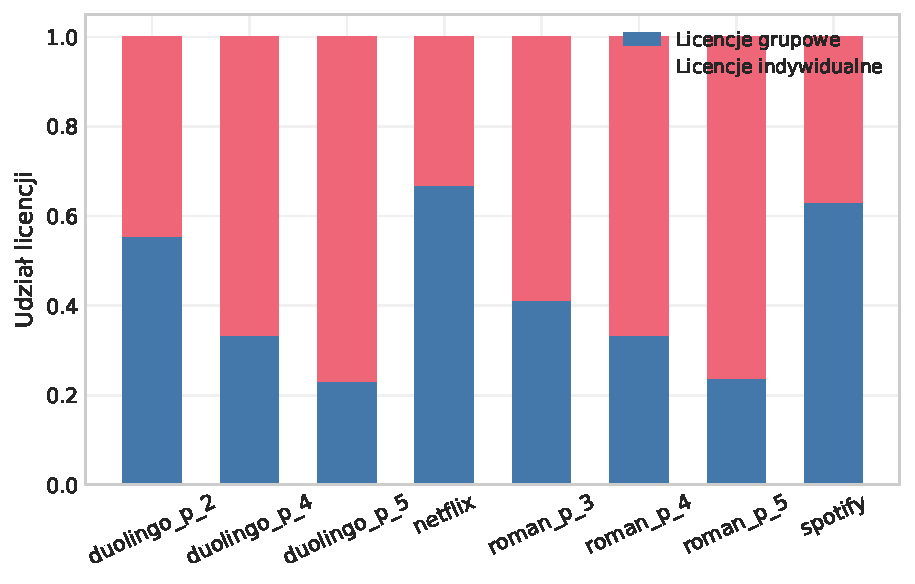
\includegraphics[width=0.8\linewidth]{assets/figures/extensions/dynamic/license_mix.pdf}
  \caption{Udział licencji grupowych i indywidualnych w rozszerzeniach dynamicznych.}
  \label{fig:ext-dynamic-license-mix}
\end{figure}

Netflix wykazuje najwyższy udział planów grupowych (67\%), co wynika z atrakcyjności planów Standard i Premium dla grup 2-4 osobowych. Ta konfiguracja stanowi wariant pośredni między licencjami indywidualnymi a planami o dużej pojemności, umożliwiając algorytmom elastyczne dopasowanie do struktury sieci.

\subsection{Porównanie z benchmarkiem statycznym}

Zestawienie wyników dynamicznych ze statycznymi (tabela~\ref{tab:ext-static-dynamic-comparison}) pokazuje ogólną zgodność trendów. Koszty w środowisku dynamicznym pozostają na podobnym poziomie -- różnice nie przekraczają 3\% dla większości konfiguracji. Czasy wykonania wydłużają się o 30-60\%, co odzwierciedla dodatkową złożoność związaną z dynamicznym rebalansowaniem.

\begin{table}[H]
  \centering
  \caption{Porównanie wyników statycznych i dynamicznych.}
  \label{tab:ext-static-dynamic-comparison}
  \begin{tabular}{lrrrr}
    \toprule
    \textbf{Konfiguracja} & \textbf{Koszt stat.} & \textbf{Koszt dyn.} & \textbf{Czas stat.} & \textbf{Czas dyn.} \\
    \midrule
    duolingo\_p\_2        & 0.554                & 0.539               & 0.637               & 0.939              \\
    duolingo\_p\_4        & 0.860                & 0.855               & 0.677               & 0.987              \\
    duolingo\_p\_5        & 0.982                & 0.980               & 0.938               & 0.980              \\
    spotify               & 0.479                & 0.467               & 0.547               & 0.881              \\
    netflix               & 0.729                & 0.714               & 0.623               & 0.891              \\
    roman\_p\_3           & 0.585                & 0.554               & 0.477               & 0.798              \\
    roman\_p\_4           & 0.701                & 0.666               & 0.475               & 0.930              \\
    roman\_p\_5           & 0.800                & 0.763               & 0.493               & 0.829              \\
    \bottomrule
  \end{tabular}
\end{table}

Najstabilniejsze wyniki wykazuje konfiguracja \texttt{duolingo\_p\_5}, gdzie koszty różnią się jedynie o 0.002 między benchmarkami. Największą poprawę w środowisku dynamicznym odnotowano dla \texttt{roman\_p\_4} (redukcja kosztu o 5\%) i \texttt{roman\_p\_5} (redukcja o 4.6\%). Może to wynikać z lepszego wykorzystania możliwości rebalansowania w mniejszych grupach charakterystycznych dla tych konfiguracji.
\section{Wnioski}

Przeprowadzone badania nad rozszerzeniami modelu licencjonowania pozwoliły na kompleksową analizę wpływu struktury cenowej na optymalizację kosztów w sieciach społecznych. Kluczowe wnioski z analizy ośmiu wariantów licencyjnych można podzielić na trzy główne obszary.

Wpływ mnożnika ceny grupowej na efektywność algorytmów. Badania wykazały wyraźną zależność między stosunkiem ceny licencji grupowej do indywidualnej a skutecznością optymalizacji. W wariantach Duolingo wzrost mnożnika z 2 do 5 powoduje zwiększenie średniego kosztu na węzeł o 77\% (z 0.554 do 0.982) oraz wydłużenie czasu obliczeń o 47\%. Podobną, choć łagodniejszą tendencję obserwuje się w wariantach dominowania rzymskiego, gdzie wzrost parametru $p$ z 3 do 5 prowadzi do 37\% wzrostu kosztu przy stabilnym czasie wykonania. Te wyniki wskazują, że metaheurystyki są najbardziej efektywne przy niskich mnożnikach, gdzie licencje grupowe pozostają opłacalne.

Znaczenie planów pośrednich w strukturze licencji. Analiza konfiguracji rzeczywistych serwisów ujawniła istotną rolę licencji o pojemności pośredniej. Spotify z planem Duo (pojemność 2) osiąga najkorzystniejszy stosunek kosztu do wydajności (0.467 kosztu na węzeł przy 0.547s czasu), podczas gdy Netflix z planem Standard oferuje skuteczne wypełnienie luki między licencjami indywidualnymi a rodzinnymi. W obu przypadkach udział licencji grupowych przekracza 63\%, co potwierdza efektywność elastycznego spektrum opcji licencyjnych.

Stabilność wyników w środowisku dynamicznym. Porównanie benchmarków statycznego i dynamicznego wykazało wysoką zgodność rezultatów -- różnice w kosztach na węzeł nie przekraczają 3\% dla większości konfiguracji. Jednocześnie zaobserwowano wzrost czasów wykonania o 30-60\%, co odzwierciedla dodatkową złożoność związaną z dynamicznym rebalansowaniem. Najstabilniejsze wyniki uzyskano w konfiguracji \texttt{duolingo\_p\_5}, gdzie różnica między środowiskami wynosi jedynie 0.002. Te obserwacje potwierdzają, że proponowane rozszerzenia modelu zachowują skuteczność w realistycznych scenariuszach z czasowymi zmianami struktury sieci.

Otrzymane wyniki mają istotne implikacje praktyczne dla projektowania systemów licencjonowania. Po pierwsze, wprowadzenie planów o pojemności pośredniej może znacząco poprawić efektywność kosztową bez zwiększenia złożoności obliczeniowej. Po drugie, przy wysokich mnożnikach ceny grupowej (powyżej 4-5) korzyści z metaheurystyk maleją, co sugeruje ekonomiczne ograniczenia optymalizacji algorytmicznej. Po trzecie, stabilność wyników w środowisku dynamicznym wskazuje na praktyczną stosowalność proponowanych rozwiązań w rzeczywistych systemach z fluktuacją użytkowników.

\chapter{Podsumowanie}\label{chap:conclusion}

\subsection{Symulacje dynamiczne}
Rozdział~\ref{chap:dynamic} opisuje symulator zmian w sieci. Uwzględnia mutacje węzłów i krawędzi oraz trzy tryby: preferencyjny, triadyczny i losowy. Zastosowanie ciepłego startu, czyli użycie poprzedniego rozwiązania, obniżało koszt względem liczenia od zera o 6--14\% na grafach syntetycznych i o 7--12\% na danych realistycznych. Czas ponownego zrównoważenia wynosił zwykle 1--3~s. Algorytm zachłanny działał w milisekundach i służył jako punkt odniesienia. Intensywność mutacji silniej wpływała na czas niż na końcowy koszt. Najwyższą dokładność uzyskiwał algorytm mrówkowy, a przeszukiwanie tabu i algorytm genetyczny dawały lepszy kompromis między kosztem i czasem. W ujęciu dynamicznym najtrudniejszy był wariant \texttt{rand\_rewire}.

Praca pokazuje pełny cykl badawczy dotyczący optymalizacji kosztów licencji grupowych w sieciach społecznościowych. Najpierw sformalizowano model. Następnie porównano algorytmy deterministyczne i metaheurystyczne. Dalej przeprowadzono symulacje dynamiczne. Na końcu rozszerzono analizę o dodatkowe plany licencyjne. Uzyskano spójny obraz działania metod w wielu scenariuszach. Poniżej zebrano główne wyniki i wskazano możliwe kierunki dalszych badań.

\section{Wyniki}

\subsection{Model i metody}
Rozdziały~\ref{chap:introduction}--\ref{chap:testdata} definiują problem jako uogólnienie dominacji rzymskiej z ograniczeniami pojemności oraz różnymi typami licencji. Wykazano wysoką złożoność obliczeniową. Rozdział~\ref{chap:algorithms} prezentuje pełen zestaw metod: dokładny solver ILP, heurystyki konstrukcyjne (m.in. algorytm zachłanny, podejście przez zbiór dominujący), metaheurystyki (algorytm genetyczny, algorytm mrówkowy, przeszukiwanie tabu, wyżarzanie symulowane) oraz algorytm losowy. Wszystkie implementacje mają wspólny interfejs, co ułatwiło porównania.

\subsection{Eksperymenty statyczne}
Rozdział~\ref{chap:experiments} potwierdza hierarchię jakości: $ILP >$ algorytm mrówkowy $>$ przeszukiwanie tabu/algorytm genetyczny $>$ wyżarzanie symulowane $>$ heurystyki konstrukcyjne $>$ algorytm losowy. Różnice są istotne statystycznie (test Friedmana oraz porównania Nemenyi'ego). Grafy bezskalowe okazały się łatwiejsze do pokrycia z powodu hubów. Czas działania metaheurystyk rósł szybko, a heurystyki konstrukcyjne utrzymywały czasy rzędu milisekund. W praktyce wyróżniono trzy zakresy: dla małych grafów warto stosować ILP jako punkt odniesienia; dla średnich grafów najlepsze są metaheurystyki; dla dużych grafów albo gdy liczy się szybkość, użyteczną aproksymację daje algorytm zachłanny.

\subsection{Symulacje dynamiczne}
Rozdział~\ref{chap:dynamic} przedstawia wpływ zmian w sieci na koszt i czas. Ciepły start konsekwentnie obniżał koszt o 6--14\% (syntetyczne) i 7--12\% (realistyczne), przy czasie rebalansowania 1--3~s. Intensywniejsze mutacje zwiększały głównie czas, a mniej wpływały na koszt. Najdokładniejszy pozostawał algorytm mrówkowy, natomiast przeszukiwanie tabu i algorytm genetyczny dawały lepszy kompromis czasowy. W danych realistycznych najniższe koszty uzyskano w wariancie Spotify (mediana $\approx 0{,}41$ na węzeł).

\subsection{Rozszerzenia licencyjne}
Rozdział~\ref{chap:extensions} analizuje osiem wariantów taryf. W planach Duolingo i Roman o opłacalności decydowały rozmiar grupy i koszt planu. Przy tańszej grupie (\texttt{duolingo\_p\_2}) metaheurystyki redukowały koszt o 10--20\% względem heurystyk. Przy droższych planach (\texttt{duolingo\_p\_5}, \texttt{roman\_p\_5}) przewaga spadała do kilku procent. Dodanie planu Duo (Spotify) oraz planów Standard/Premium (Netflix) umożliwiło nowe parowania użytkowników i obniżyło koszt na węzeł (mediana 0{,}40 w Spotify wobec 0{,}50 w \texttt{duolingo\_p\_2}). W dynamice konfiguracje z planem pośrednim utrzymywały najkorzystniejszy koszt i stabilny czas, a metaheurystyki dawały 5--12\% oszczędności względem algorytmu zachłannego.

\section{Rekomendacje praktyczne}

\textbf{Dobór algorytmu.} Dla instancji do około 200 węzłów solver ILP jest najlepszym punktem odniesienia. Dla większych sieci zalecane są algorytm mrówkowy albo przeszukiwanie tabu; w środowisku dynamicznym krótsze czasy rebalansowania daje przeszukiwanie tabu.

\textbf{Strategia inicjalizacji.} Ciepły start metaheurystyk, czyli start z poprzedniego rozwiązania, obniża koszt o 6--14\% przy niewielkim koszcie czasowym. W systemach aktualizowanych częściowo powinien to być standard.

\textbf{Polityka licencyjna.} Tańsze plany rodzinne, w szczególności warianty pośrednie (np. Duo), realnie zmniejszają koszt końcowy. Zbyt wysokie $p$ w planach grupowych sprzyja licencjom indywidualnym i ogranicza zyski z optymalizacji.

\section{Kierunki dalszych badań}

\textbf{Gwarancje aproksymacji.} Warto poszukać teoretycznych ograniczeń jakości rozwiązań dla wybranych klas grafów lub modeli losowych.
\textbf{Modele stochastyczne.} Ujęcie niepewności w dostępie użytkowników i ewolucji sieci może zwiększyć odporność rozwiązań (np. podejścia dwuetapowe lub bayesowskie).
\textbf{Wielokryterialność i koszty operacyjne.} Rozszerzenie funkcji celu o sprawiedliwość, ryzyko czy koszt migracji lepiej odzwierciedli praktykę.
\textbf{Optymalizacja hiperparametrów.} Automatyczne strojenie parametrów metaheurystyk (np. techniki z rodziny AutoML) może poprawić stosunek kosztu do czasu bez ręcznego dostrajania.
\textbf{Integracja z praktyką.} Biblioteka daje podstawy do wdrożeń w systemach rekomendacji planów rodzinnych; naturalnym krokiem jest eksperyment online na rzeczywistych danych.

\section{Zakończenie}

Przedstawiony model, zestaw algorytmów oraz eksperymenty statyczne i dynamiczne pokazują, że mimo wysokiej złożoności można uzyskać rozwiązania dobrej jakości w akceptowalnym czasie. Kluczowy jest dobór metody do wielkości i dynamiki sieci oraz rozsądna polityka licencyjna. Wyniki stanowią podstawę do dalszych prac oraz do zastosowań w usługach subskrypcyjnych, gdzie modele rodzinne stają się standardem.


\printbibliography

% Wpis dot. użycia narzędzi GenAI zgodnie z wytycznymi PG
\nocite{genai_usage}

% Appendices (additional materials, calculations, etc.)
% \appendix
% \chapter{Wybrane fragmenty implementacji}

\section{Organizacja skryptów eksperymentalnych}
Środowisko obliczeniowe zorganizowano jako spójny zestaw modułów
Pythona: pakiety do benchmarków statycznych, osobne moduły do
symulacji dynamicznych i rozszerzeń, a także proste komendy CLI do
szybkiej diagnostyki pojedynczych algorytmów. Wspólny rdzeń dba o
jednolite budowanie i walidację rozwiązań, a skrypty analityczne
tworzą raporty i wykresy użyte w częściach eksperymentalnych.

\section{Algorytmy dokładne}
\subsection{Program całkowitoliczbowy}
Pełna implementacja solvera ILP wykorzystującego bibliotekę PuLP
z solverem CBC do wyznaczania rozwiązań wzorcowych.

    {\footnotesize
        \begin{verbatim}
class ILPSolver(Algorithm):
    def solve(self, graph: nx.Graph, license_types: Sequence[LicenseType], **kwargs) -> Solution:
        # G = (V,E), N[i] = neighbors(i) union {i}
        nodes: list[Any] = list(graph.nodes())
        Nhood: dict[Any, set[Any]] = {i: set(graph.neighbors(i)) | {i} for i in nodes}
        degp1: dict[Any, int] = {i: len(Nhood[i]) for i in nodes}

        model = pulp.LpProblem("graph_licensing_optimization", pulp.LpMinimize)

        # active[i,t] = 1 gdy wlasciciel i otwiera grupe typu t
        active: dict[tuple[Any, int], pulp.LpVariable] = {}
        for i in nodes:
            for t_idx, lt in enumerate(license_types):
                feasible_owner_type = (lt.min_capacity <= degp1[i]) and (lt.max_capacity >= 1)
                if feasible_owner_type:
                    active[i, t_idx] = pulp.LpVariable(f"a_{i}_{t_idx}", cat="Binary")
                else:
                    # eliminacja niemozliwych par i,t
                    active[i, t_idx] = pulp.LpVariable(f"a_{i}_{t_idx}", lowBound=0, upBound=0, cat="Binary")

        # assign[i,j,t] = 1 gdy j nalezy do grupy wlasciciela i typu t
        assign: dict[tuple[Any, Any, int], pulp.LpVariable] = {}
        for i in nodes:
            for t_idx, lt in enumerate(license_types):
                if active[i, t_idx].upBound == 0:
                    continue
                if lt.max_capacity == 1:
                    # typ indywidualny, tylko wlasciciel
                    assign[i, i, t_idx] = pulp.LpVariable(f"x_{i}_{i}_{t_idx}", cat="Binary")
                else:
                    for j in Nhood[i]:
                        assign[i, j, t_idx] = pulp.LpVariable(f"x_{i}_{j}_{t_idx}", cat="Binary")

        # cel: min sum c_t * active[i,t]
        model += pulp.lpSum(active[i, t_idx] * license_types[t_idx].cost for i in nodes
                           for t_idx in range(len(license_types)))

        # co najwyzej jedna licencja na wlasciciela
        for i in nodes:
            model += pulp.lpSum(active[i, t_idx] for t_idx in range(len(license_types))) <= 1

        # pokrycie dokladnie raz
        for j in nodes:
            model += pulp.lpSum(assign.get((i, j, t_idx), 0) for i in Nhood[j]
                               for t_idx in range(len(license_types))) == 1

        # sprzezenie i pojemnosc
        for i in nodes:
            for t_idx, lt in enumerate(license_types):
                if active[i, t_idx].upBound == 0:
                    continue
                # wlasciciel nalezy do swojej grupy
                model += assign.get((i, i, t_idx), 0) == active[i, t_idx]
                # brak przypisan bez aktywacji
                for j in Nhood[i]:
                    var = assign.get((i, j, t_idx))
                    if var is not None:
                        model += var <= active[i, t_idx]
                # min i max pojemnosci tylko gdy aktywna
                group_size = pulp.lpSum(assign.get((i, j, t_idx), 0) for j in Nhood[i])
                model += group_size <= active[i, t_idx] * lt.max_capacity
                model += group_size >= active[i, t_idx] * lt.min_capacity

        # rozwiazanie ilp
        solver = pulp.PULP_CBC_CMD(msg=False)
        model.solve(solver)
        status = pulp.LpStatus.get(model.status, "Unknown")

        # fallback gdy brak rozwiazania dopuszczalnego
        if status in ("Infeasible", "Undefined", "Unbounded", "Not Solved"):
            singles = [lt for lt in license_types if lt.min_capacity <= 1 <= lt.max_capacity]
            if not singles:
                raise RuntimeError(f"ILP {status}: no single license available")
            lt = min(singles, key=lambda x: x.cost)
            groups = [LicenseGroup(license_type=lt, owner=i, additional_members=frozenset()) for i in nodes]
            return Solution(groups=tuple(groups))

        # ekstrakcja rozwiazania
        groups = []
        for i in nodes:
            for t_idx, lt in enumerate(license_types):
                a = active.get((i, t_idx))
                a_val = float(a.varValue) if a is not None and a.varValue is not None else 0.0
                if a_val > 0.5:
                    members: set[Any] = set()
                    for j in Nhood[i]:
                        var = assign.get((i, j, t_idx))
                        v_val = float(var.varValue) if var is not None and var.varValue is not None else 0.0
                        if v_val > 0.5:
                            members.add(j)
                    if members:
                        groups.append(
                            LicenseGroup(
                                license_type=lt,
                                owner=i,
                                additional_members=frozenset(members - {i}),
                            )
                        )

        return Solution(groups=tuple(groups))
\end{verbatim}
    }

\section{Algorytmy metaheurystyczne}
\subsection{Algorytm genetyczny}
Główne fragmenty implementacji algorytmu genetycznego z elityzmem,
selekcją turniejową oraz operatorami krzyżowania i mutacji.

    {\footnotesize
        \begin{verbatim}
class GeneticAlgorithm(Algorithm):
    def __init__(self, population_size: int = 30, num_generations: int = 40,
                 elite_fraction: float = 0.2, crossover_rate: float = 0.6):
        self.population_size = max(2, population_size)
        self.num_generations = max(1, num_generations)
        self.elite_fraction = max(0.0, min(1.0, elite_fraction))
        self.crossover_rate = max(0.0, min(1.0, crossover_rate))
        self.validator = SolutionValidator()

    def solve(self, graph: nx.Graph, license_types: Sequence[LicenseType], **kwargs) -> Solution:
        population = self._init_population(graph, license_types, initial)
        best = min(population, key=lambda s: s.total_cost)

        for _ in range(num_generations):
            population.sort(key=lambda s: s.total_cost)
            elite_count = max(1, int(self.elite_fraction * self.population_size))
            new_pop: list[Solution] = population[:elite_count]

            while len(new_pop) < self.population_size:
                if random.random() < self.crossover_rate and len(population) >= 2:
                    p1 = self._tournament_selection(population)
                    p2 = self._tournament_selection(population)
                    child = self._crossover(p1, p2, graph, license_types)
                    if not self.validator.is_valid_solution(child, graph):
                        base = min([p1, p2], key=lambda s: s.total_cost)
                        child = self._mutate(base, graph, license_types)
                else:
                    parent = self._tournament_selection(population)
                    child = self._mutate(parent, graph, license_types)
                new_pop.append(child)

            population = new_pop
            current_best = min(population, key=lambda s: s.total_cost)
            if current_best.total_cost < best.total_cost:
                best = current_best
        return best

    def _crossover(self, p1: Solution, p2: Solution, graph: nx.Graph,
                   license_types: Sequence[LicenseType]) -> Solution:
        def eff(g):
            return (g.license_type.cost / max(1, g.size), -g.size)

        candidates = list(p1.groups) + list(p2.groups)
        candidates.sort(key=eff)
        used = set()
        chosen: list = []
        for g in candidates:
            if used.isdisjoint(g.all_members):
                chosen.append(g)
                used.update(g.all_members)

        # Domknięcie niepokrytych węzłów algorytmem zachłannym
        uncovered = set(graph.nodes()) - used
        if uncovered:
            H = graph.subgraph(uncovered)
            filler = GreedyAlgorithm().solve(H, list(license_types))
            for fg in filler.groups:
                if set(fg.all_members).issubset(uncovered):
                    chosen.append(fg)

        child = SolutionBuilder.create_solution_from_groups(chosen)
        if not self.validator.is_valid_solution(child, graph):
            return GreedyAlgorithm().solve(graph, list(license_types))
        return child

    def _mutate(self, solution: Solution, graph: nx.Graph,
                license_types: Sequence[LicenseType]) -> Solution:
        neighbors = MutationOperators.generate_neighbors(solution, graph, license_types, k=5)
        valid_neighbors = [s for s in neighbors if self.validator.is_valid_solution(s, graph)]
        if not valid_neighbors:
            return solution
        return min(valid_neighbors, key=lambda s: s.total_cost)
\end{verbatim}
    }

\subsection{Optymalizacja mrówkowa}
Kluczowe fragmenty algorytmu mrówkowego z konstrukcją rozwiązań
oraz aktualizacją śladu feromonowego.

    {\footnotesize
        \begin{verbatim}
class AntColonyOptimization(Algorithm):
    def __init__(self, alpha: float = 1.0, beta: float = 2.0, evaporation: float = 0.5,
                 q0: float = 0.9, num_ants: int = 20):
        self.alpha, self.beta, self.evap, self.q0, self.num_ants = alpha, beta, evaporation, q0, num_ants

    def solve(self, graph: nx.Graph, license_types: Sequence[LicenseType], **kwargs) -> Solution:
        pher = self._init_pher(graph, license_types)  # Inicjalizacja feromonu
        heur = self._init_heur(graph, license_types)  # Informacja heurystyczna
        best = GreedyAlgorithm().solve(graph, license_types)
        self._deposit(pher, best)

        for _ in range(max_iter_aco):
            improved = False
            for _ in range(num_ants):
                cand = self._construct(graph, license_types, pher, heur)
                ok, _ = self.validator.validate(cand, graph)
                if ok and cand.total_cost < best.total_cost:
                    best, improved = cand, True
            self._evaporate(pher)
            self._deposit(pher, best)
        return best

    def _construct(self, graph: nx.Graph, lts: Sequence[LicenseType],
                   pher: dict, heur: dict) -> Solution:
        uncovered: set[Any] = set(graph.nodes())
        groups: list[LicenseGroup] = []

        while uncovered:
            owner = self._select_owner(uncovered, lts, pher, heur)
            lt = self._select_license(owner, lts, pher, heur)

            pool = (set(graph.neighbors(owner)) | {owner}) & uncovered
            if len(pool) < lt.min_capacity:
                # Fallback do licencji indywidualnej
                singles = [x for x in lts if x.min_capacity <= 1 <= x.max_capacity]
                lt = min(singles, key=lambda x: x.cost) if singles else lt
                groups.append(LicenseGroup(lt, owner, frozenset()))
                uncovered.remove(owner)
                continue

            # Wybór członków grupy według stopnia
            k = max(0, lt.max_capacity - 1)
            add = sorted((pool - {owner}), key=lambda n: graph.degree[n], reverse=True)[:k]
            groups.append(LicenseGroup(lt, owner, frozenset(add)))
            uncovered -= {owner} | set(add)

        return Solution(groups=tuple(groups))

    def _select_owner(self, uncovered: set, lts: Sequence[LicenseType],
                      pher: dict, heur: dict) -> Any:
        scores = {}
        for n in uncovered:
            acc = sum((pher.get((n, lt.name), 1.0) ** self.alpha) *
                     (heur.get((n, lt.name), 1.0) ** self.beta) for lt in lts)
            scores[n] = acc / max(1, len(lts))
        return self._roulette_or_best(list(uncovered), scores)

    def _evaporate(self, pher: dict) -> None:
        for k in pher:
            pher[k] *= (1.0 - self.evap)

    def _deposit(self, pher: dict, sol: Solution) -> None:
        if sol.total_cost > 0:
            q = 1.0 / sol.total_cost
            for g in sol.groups:
                for n in g.all_members:
                    k = (n, g.license_type.name)
                    if k in pher:
                        pher[k] += q
\end{verbatim}
    }

\subsection{Wyżarzanie symulowane}
Fragment implementacji wyżarzania z generowaniem sąsiadów
i akceptacją według kryterium Metropolisa.

    {\footnotesize
        \begin{verbatim}
class SimulatedAnnealing(Algorithm):
    def solve(self, graph: nx.Graph, license_types: Sequence[LicenseType], **kwargs) -> Solution:
        current = GreedyAlgorithm().solve(graph, license_types)
        best = current
        temp = self.temp_initial
        stall = 0

        for _ in range(self.max_iterations):
            if temp < self.temp_min:
                break

            cand = self._neighbor(current, graph, license_types)
            if cand is None:
                stall += 1
            else:
                delta = cand.total_cost - current.total_cost
                if delta < 0 or random.random() < math.exp(-delta / max(temp, 1e-10)):
                    current = cand
                    if current.total_cost < best.total_cost:
                        best, stall = current, 0
                    else:
                        stall += 1
                else:
                    stall += 1

            if stall >= self.max_stall:
                stall, temp = 0, max(self.temp_min, 0.5 * temp)
            temp *= self.cooling_rate

        return best

    def _neighbor(self, solution: Solution, graph: nx.Graph, lts: Sequence[LicenseType]) -> Solution:
        moves = [self._mv_change_license, self._mv_move_member,
                 self._mv_swap_members, self._mv_merge_groups, self._mv_split_group]

        for _ in range(12):
            mv = random.choice(moves)
            try:
                cand = mv(solution, graph, lts)
                if cand and self.validator.validate(cand, graph)[0]:
                    return cand
            except Exception:
                continue
        return None
\end{verbatim}
    }

\section{Operatory mutacji i sąsiedztwa}
Kluczowe operatory używane przez metaheurystyki do generowania
sąsiadów i eksploracji przestrzeni rozwiązań.

{\footnotesize
\begin{verbatim}
class MutationOperators:
    @staticmethod
    def generate_neighbors(base: Solution, graph: nx.Graph,
                          license_types: Sequence[LicenseType], k: int = 10) -> list[Solution]:
        ops = (MutationOperators.change_license_type, MutationOperators.reassign_member,
               MutationOperators.merge_groups, MutationOperators.split_group)
        weights = (0.3, 0.3, 0.2, 0.2)
        out: list[Solution] = []
        attempts = 0

        while len(out) < k and attempts < k * 10:
            attempts += 1
            op = random.choices(ops, weights=weights, k=1)[0]
            try:
                cand = op(base, graph, list(license_types))
                if cand is not None:
                    out.append(cand)
            except Exception:
                continue
        return out

    @staticmethod
    def change_license_type(solution: Solution, graph: nx.Graph,
                           license_types: list[LicenseType]) -> Solution | None:
        if not solution.groups:
            return None
        group = random.choice(solution.groups)
        compatible = SolutionBuilder.get_compatible_license_types(
            group.size, license_types, exclude=group.license_type
        )
        if not compatible:
            return None

        new_lt = random.choice(compatible)
        new_groups = []
        for g in solution.groups:
            if g is group:
                new_groups.append(LicenseGroup(new_lt, g.owner, g.additional_members))
            else:
                new_groups.append(g)
        return SolutionBuilder.create_solution_from_groups(new_groups)

    @staticmethod
    def reassign_member(solution: Solution, graph: nx.Graph,
                       license_types: list[LicenseType]) -> Solution | None:
        if len(solution.groups) < 2:
            return None

        donors = [g for g in solution.groups
                 if g.size > g.license_type.min_capacity and g.additional_members]
        receivers = [g for g in solution.groups if g.size < g.license_type.max_capacity]

        if not donors or not receivers:
            return None

        from_group = random.choice(donors)
        pot_receivers = [g for g in receivers if g is not from_group]
        if not pot_receivers:
            return None

        to_group = random.choice(pot_receivers)
        member = random.choice(list(from_group.additional_members))
        allowed = SolutionBuilder.get_owner_neighbors_with_self(graph, to_group.owner)

        if member not in allowed:
            return None

        # Przeprowadzenie transferu
        new_groups = []
        for g in solution.groups:
            if g is from_group:
                new_groups.append(LicenseGroup(
                    g.license_type, g.owner, g.additional_members - {member}
                ))
            elif g is to_group:
                new_groups.append(LicenseGroup(
                    g.license_type, g.owner, g.additional_members | {member}
                ))
            else:
                new_groups.append(g)

        return SolutionBuilder.create_solution_from_groups(new_groups)

    @staticmethod
    def split_group(solution: Solution, graph: nx.Graph,
                   license_types: list[LicenseType]) -> Solution | None:
        splittable = [g for g in solution.groups if g.size > 2]
        if not splittable:
            return None

        group = random.choice(splittable)
        members = list(group.all_members)

        for _ in range(4):  # Próbuj kilka podziałów
            random.shuffle(members)
            cut = random.randint(1, len(members) - 1)
            part1, part2 = members[:cut], members[cut:]

            # Sprawdź kompatybilność typów licencji
            compat1 = SolutionBuilder.get_compatible_license_types(len(part1), license_types)
            compat2 = SolutionBuilder.get_compatible_license_types(len(part2), license_types)

            if not compat1 or not compat2:
                continue

            # Wybierz właścicieli i typy licencji
            owner1, owner2 = random.choice(part1), random.choice(part2)
            lt1, lt2 = min(compat1, key=lambda x: x.cost), min(compat2, key=lambda x: x.cost)

            # Sprawdź ograniczenia sąsiedztwa
            if (set(part1).issubset(SolutionBuilder.get_owner_neighbors_with_self(graph, owner1)) and
                set(part2).issubset(SolutionBuilder.get_owner_neighbors_with_self(graph, owner2))):

                new_groups = [g for g in solution.groups if g is not group]
                new_groups.append(LicenseGroup(lt1, owner1, frozenset(set(part1) - {owner1})))
                new_groups.append(LicenseGroup(lt2, owner2, frozenset(set(part2) - {owner2})))
                return SolutionBuilder.create_solution_from_groups(new_groups)

        return None
\end{verbatim}
}

\section{Funkcje pomocnicze}
\subsection{Budowanie i walidacja rozwiązań}
Klasy pomocnicze odpowiedzialne za tworzenie i weryfikację poprawności rozwiązań.

{\footnotesize
\begin{verbatim}
class SolutionBuilder:
    @staticmethod
    def get_compatible_license_types(group_size: int, license_types: Sequence[LicenseType],
                                   exclude: LicenseType | None = None) -> list[LicenseType]:
        out: list[LicenseType] = []
        for lt in license_types:
            if exclude and lt == exclude:
                continue
            if lt.min_capacity <= group_size <= lt.max_capacity:
                out.append(lt)
        return out

    @staticmethod
    def get_owner_neighbors_with_self(graph: nx.Graph, owner: N) -> set[N]:
        return set(graph.neighbors(owner)) | {owner}

    @staticmethod
    def find_cheapest_single_license(license_types: Sequence[LicenseType]) -> LicenseType:
        singles = [lt for lt in license_types if lt.min_capacity <= 1]
        return min(singles or list(license_types), key=lambda lt: lt.cost)

class SolutionValidator:
    def validate(self, solution: Solution[N], graph: nx.Graph) -> tuple[bool, list[ValidationIssue]]:
        issues: list[ValidationIssue] = []
        nodes = set(graph.nodes())
        groups = tuple(solution.groups)

        # Sprawdzanie członków grup
        issues += self._check_group_members(groups, nodes)
        # Sprawdzanie pojemności licencji
        issues += self._check_group_capacity(groups)
        # Sprawdzanie ograniczeń sąsiedztwa
        issues += self._check_neighbors(groups, graph, nodes)
        # Sprawdzanie braku nakładania się grup
        issues += self._check_no_overlap(groups)
        # Sprawdzanie pokrycia wszystkich węzłów
        issues += self._check_coverage(groups, nodes)

        return (not issues, issues)

    def _check_neighbors(self, groups: tuple[LicenseGroup[N], ...], graph: nx.Graph,
                        nodes: set[N]) -> list[ValidationIssue]:
        issues: list[ValidationIssue] = []
        for idx, g in enumerate(groups):
            if g.owner not in nodes:
                continue
            allowed_any = set(graph.neighbors(g.owner)) | {g.owner}
            not_neighbors = set(g.all_members) - allowed_any
            if not_neighbors:
                issues.append(ValidationIssue(
                    "DISCONNECTED_MEMBER",
                    f"group#{idx} owner {g.owner!r} has non-neighbor members: {list(not_neighbors)!r}"
                ))
        return issues

    def _check_coverage(self, groups: tuple[LicenseGroup[N], ...], nodes: set[N]) -> list[ValidationIssue]:
        issues: list[ValidationIssue] = []
        covered = set().union(*(set(g.all_members) for g in groups)) if groups else set()
        missing = nodes - covered
        if missing:
            issues.append(ValidationIssue("MISSING_COVERAGE", f"missing nodes: {list(missing)!r}"))
        return issues
\end{verbatim}
}

\subsection{Konfiguracje licencyjne}
Fabryka konfiguracji licencyjnych obsługująca różne rodziny
licencji oraz dynamiczne warianty cenowe.

    {\footnotesize
        \begin{verbatim}
class LicenseConfigFactory:
    _CONFIGS: ClassVar[dict[str, Callable[[], list[LicenseType]]]] = {
        "duolingo_super": lambda: [
            LicenseType("Individual", 13.99, 1, 1, LicenseConfigFactory.BLACK),
            LicenseType("Family", 29.17, 2, 6, LicenseConfigFactory.BLACK),
        ],
        "spotify": lambda: [
            LicenseType("Individual", 23.99, 1, 1, LicenseConfigFactory.RED),
            LicenseType("Duo", 30.99, 2, 2, LicenseConfigFactory.GREEN),
            LicenseType("Family", 37.99, 2, 6, LicenseConfigFactory.BLUE),
        ],
        "netflix": lambda: [
            LicenseType("Basic", 33, 1, 1, LicenseConfigFactory.RED),
            LicenseType("Standard", 49, 1, 2, LicenseConfigFactory.GREEN),
            LicenseType("Premium", 67, 1, 4, LicenseConfigFactory.BLUE),
        ],
        "roman_domination": lambda: [
            LicenseType("Solo", 1.0, 1, 1, LicenseConfigFactory.BLUE),
            LicenseType("Group", 2.0, 2, 999999, LicenseConfigFactory.RED),
        ],
    }

    @classmethod
    def get_config(cls, name: str) -> list[LicenseType]:
        # Obsługa dynamicznych wariantów roman_p_<price>
        if name.startswith("roman_p_"):
            p_str = name.split("_", 2)[2].replace("_", ".")
            try:
                p_val = float(p_str)
                return [
                    LicenseType("Solo", 1.0, 1, 1, cls.BLUE),
                    LicenseType("Group", p_val, 2, 999999, cls.RED),
                ]
            except Exception:
                raise ValueError(f"Invalid roman price format: {name}")

        # Obsługa dynamicznych wariantów duolingo_p_<price>
        if name.startswith("duolingo_p_"):
            p_str = name.split("_", 2)[2].replace("_", ".")
            try:
                p_val = float(p_str)
                return [
                    LicenseType("Individual", 1.0, 1, 1, cls.RED),
                    LicenseType("Family", p_val, 2, 6, cls.BLUE),
                ]
            except Exception:
                raise ValueError(f"Invalid duolingo price format: {name}")

        # Konfiguracje statyczne
        try:
            return cls._CONFIGS[name]()
        except KeyError:
            available = ", ".join(cls._CONFIGS.keys())
            raise ValueError(f"Unsupported license config: {name}. Available: {available}")
\end{verbatim}
    }

\section{Symulacja dynamiczna}
\subsection{Symulator ewolucji sieci}
Główne komponenty symulatora odpowiedzialnego za mutacje
struktury grafu w eksperymentach dynamicznych.

    {\footnotesize
        \begin{verbatim}
@dataclass
class MutationParams:
    add_nodes_prob: float = 0.1
    remove_nodes_prob: float = 0.05
    add_edges_prob: float = 0.15
    remove_edges_prob: float = 0.1
    max_nodes_add: int = 3
    max_nodes_remove: int = 2
    max_edges_add: int = 5
    max_edges_remove: int = 3
    mode_nodes: str = "random"      # "random" lub "preferential"
    mode_edges: str = "random"      # "random", "preferential", "triadic", "rewire_ws"
    add_node_attach_m: int = 2
    triadic_trials: int = 20

class DynamicNetworkSimulator:
    def __init__(self, mutation_params: MutationParams | None = None, seed: int | None = None):
        self.mutation_params = mutation_params or MutationParams()
        self.next_node_id = 0
        if seed is not None:
            random.seed(seed)

    def _apply_mutations(self, graph: nx.Graph) -> tuple[nx.Graph, list[str]]:
        mutations = []

        # Dodawanie węzłów
        if random.random() < self.mutation_params.add_nodes_prob:
            num_add = random.randint(1, self.mutation_params.max_nodes_add)
            new_nodes = self._add_nodes(graph, num_add)
            mutations.append(f"Added nodes: {new_nodes}")

        # Usuwanie węzłów (z zachowaniem minimalnego rozmiaru)
        if (random.random() < self.mutation_params.remove_nodes_prob
            and graph.number_of_nodes() > 5):
            num_remove = random.randint(1, min(self.mutation_params.max_nodes_remove,
                                              graph.number_of_nodes() - 5))
            removed_nodes = self._remove_nodes(graph, num_remove)
            mutations.append(f"Removed nodes: {removed_nodes}")

        # Dodawanie krawędzi
        if random.random() < self.mutation_params.add_edges_prob:
            num_add = random.randint(1, self.mutation_params.max_edges_add)
            if self.mutation_params.mode_edges == "rewire_ws":
                added_c, removed_c = self._rewire_edges(graph, num_add)
                if added_c: mutations.append(f"Added {added_c} edges")
                if removed_c: mutations.append(f"Removed {removed_c} edges")
            else:
                added_edges = self._add_edges(graph, num_add)
                mutations.append(f"Added {len(added_edges)} edges")

        return (graph, mutations)

    def _add_nodes(self, graph: nx.Graph, num_nodes: int) -> list[int]:
        new_nodes = []
        existing_nodes = list(graph.nodes())

        for _ in range(num_nodes):
            new_node = self.next_node_id
            self.next_node_id += 1
            graph.add_node(new_node)
            new_nodes.append(new_node)

            # Podłączanie do istniejących węzłów
            if existing_nodes:
                m = min(self.mutation_params.add_node_attach_m, len(existing_nodes))

                if self.mutation_params.mode_nodes == "preferential":
                    # Attachment proporcjonalny do stopni węzłów
                    deg = graph.degree
                    weights = [deg[v] + 1 for v in existing_nodes]
                    total = sum(weights)
                    chosen = set()

                    for _ in range(m):
                        if not existing_nodes: break
                        r = random.uniform(0, total)
                        acc, pick_idx = 0.0, 0
                        for idx, w in enumerate(weights):
                            acc += w
                            if acc >= r:
                                pick_idx = idx
                                break
                        v = existing_nodes[pick_idx]
                        if v not in chosen:
                            graph.add_edge(new_node, v)
                            chosen.add(v)
                        total -= weights[pick_idx]
                        existing_nodes.pop(pick_idx)
                        weights.pop(pick_idx)
                else:
                    # Losowe podłączanie
                    neighbors = random.sample(existing_nodes, m)
                    for neighbor in neighbors:
                        graph.add_edge(new_node, neighbor)

            existing_nodes = list(graph.nodes())

        return new_nodes

    def _add_edges(self, graph: nx.Graph, num_edges: int) -> list[tuple[int, int]]:
        nodes = list(graph.nodes())
        added_edges = []
        if len(nodes) < 2: return added_edges

        mode = self.mutation_params.mode_edges
        if mode == "triadic":
            # Zamykanie trójkątów
            attempts = 0
            while len(added_edges) < num_edges and attempts < num_edges * 20:
                w = random.choice(nodes)
                neigh = list(graph.neighbors(w))
                if len(neigh) >= 2:
                    u, v = random.sample(neigh, 2)
                    if not graph.has_edge(u, v):
                        graph.add_edge(u, v)
                        added_edges.append((u, v))
                attempts += 1

        elif mode == "preferential":
            # Preferencyjne dodawanie proporcjonalne do iloczynów stopni
            attempts = 0
            while len(added_edges) < num_edges and attempts < num_edges * 20:
                u, v = random.sample(nodes, 2)
                if graph.has_edge(u, v):
                    attempts += 1
                    continue
                deg = graph.degree
                w = (deg[u] + 1) * (deg[v] + 1)
                max_deg = max((deg[x] for x in nodes), default=1)
                accept_p = min(1.0, w / float((max_deg + 1) ** 2))
                if random.random() < accept_p:
                    graph.add_edge(u, v)
                    added_edges.append((u, v))
                attempts += 1

        return added_edges
\end{verbatim}
    }


\end{document}
